% Created 2021-08-05 Thu 12:48
% Intended LaTeX compiler: pdflatex
\documentclass[presentation, smaller]{beamer}
\usepackage[utf8]{inputenc}
\usepackage[T1]{fontenc}
\usepackage{graphicx}
\usepackage{grffile}
\usepackage{longtable}
\usepackage{wrapfig}
\usepackage{rotating}
\usepackage[normalem]{ulem}
\usepackage{amsmath}
\usepackage{textcomp}
\usepackage{amssymb}
\usepackage{capt-of}
\usepackage{hyperref}
\author{Willy Rempel}
\beamertemplatenavigationsymbolsempty
\setbeamertemplate{headline}{}
\setbeamersize{text margin left=0pt,text margin right=0pt}
\usepackage{amsmath, amsthm, amssymb}
\usepackage{verbatim, appendix}
\usepackage{ulem}
\usepackage{graphicx}
\usepackage{caption}
\usepackage{pseudocode}
\usepackage[ruled]{algorithm2e}
\usepackage{array}
\usepackage{booktabs}
\usepackage{listings}
\usepackage[]{biblatex}
\setbeamertemplate{bibliography item}{\insertbiblabel}
\AtEveryBibitem{\clearfield{note}}
\bibliography{AlphafoldTalk2021.bib}
\usetheme{Rochester}
\usecolortheme{dolphin}
\date{Saturday, July 24, 2021}
\title{Highly accurate protein structure prediction with AlphaFold}
\subtitle{AISC Healthcare Discussion Group}
\graphicspath{{./imgs/}}
\hypersetup{
 pdfauthor={Willy Rempel},
 pdftitle={Highly accurate protein structure prediction with AlphaFold},
 pdfkeywords={},
 pdfsubject={},
 pdfcreator={Emacs 28.0.50 (Org mode 9.4.1)}, 
 pdflang={English}}
\begin{document}

\maketitle
\section*{Introduction}
\label{sec:org4f5f3b0}
\begin{frame}[label={sec:org4a4fa45}]{Introduction}
\begin{columns}
\begin{column}{0.4\columnwidth}
\begin{center}
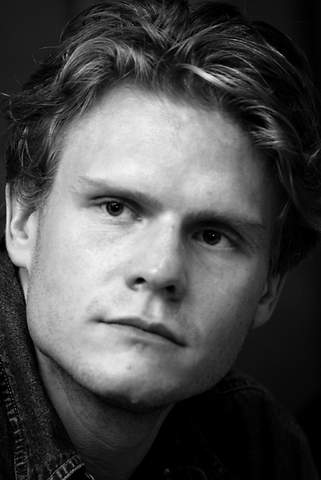
\includegraphics[scale=0.3]{./imgs/profilepic2.jpg}
\end{center}
\end{column}
\begin{column}{0.6\columnwidth}
Willy Rempel
\begin{itemize}
\item HBSc Computer Science \\
\item BSc Mathematics \\
\item Research Associate, AISC \\
\item seeking opportunities in the field
\end{itemize}
\end{column}
\end{columns}
\end{frame}
\begin{frame}[label={sec:org867dfa4}]{Introduction}
\begin{quote}
Although all of the ideas in the model are doubtlessly clever, the main secret behind AlphaFold 2’s success is the superb deep learning engineering. A close look at the model reveals an architecture with a large amount of small details that seem fundamental for the performance of the network. As we admire the end product, we should not turn a blind eye to the enormous budget, and the large team of full-time, handsomely paid engineers that made it possible.  \cite{rubieraAlphaFoldHereWhat}
\end{quote}

\begin{quote}
This, and many other tricks, are described in exhaustive detail in the Supplementary Information. A reduced subset has been analysed in a brief ablation study, but ultimately, how important are each of the minor details is anybody’s guess.  \cite{rubieraAlphaFoldHereWhat}
\end{quote}

\flushright{(above blog post is recommended reading)}
\end{frame}
\begin{frame}[label={sec:orgebb2e77}]{Model Overview \cite{jumperHighlyAccurateProtein2021}}
\begin{center}
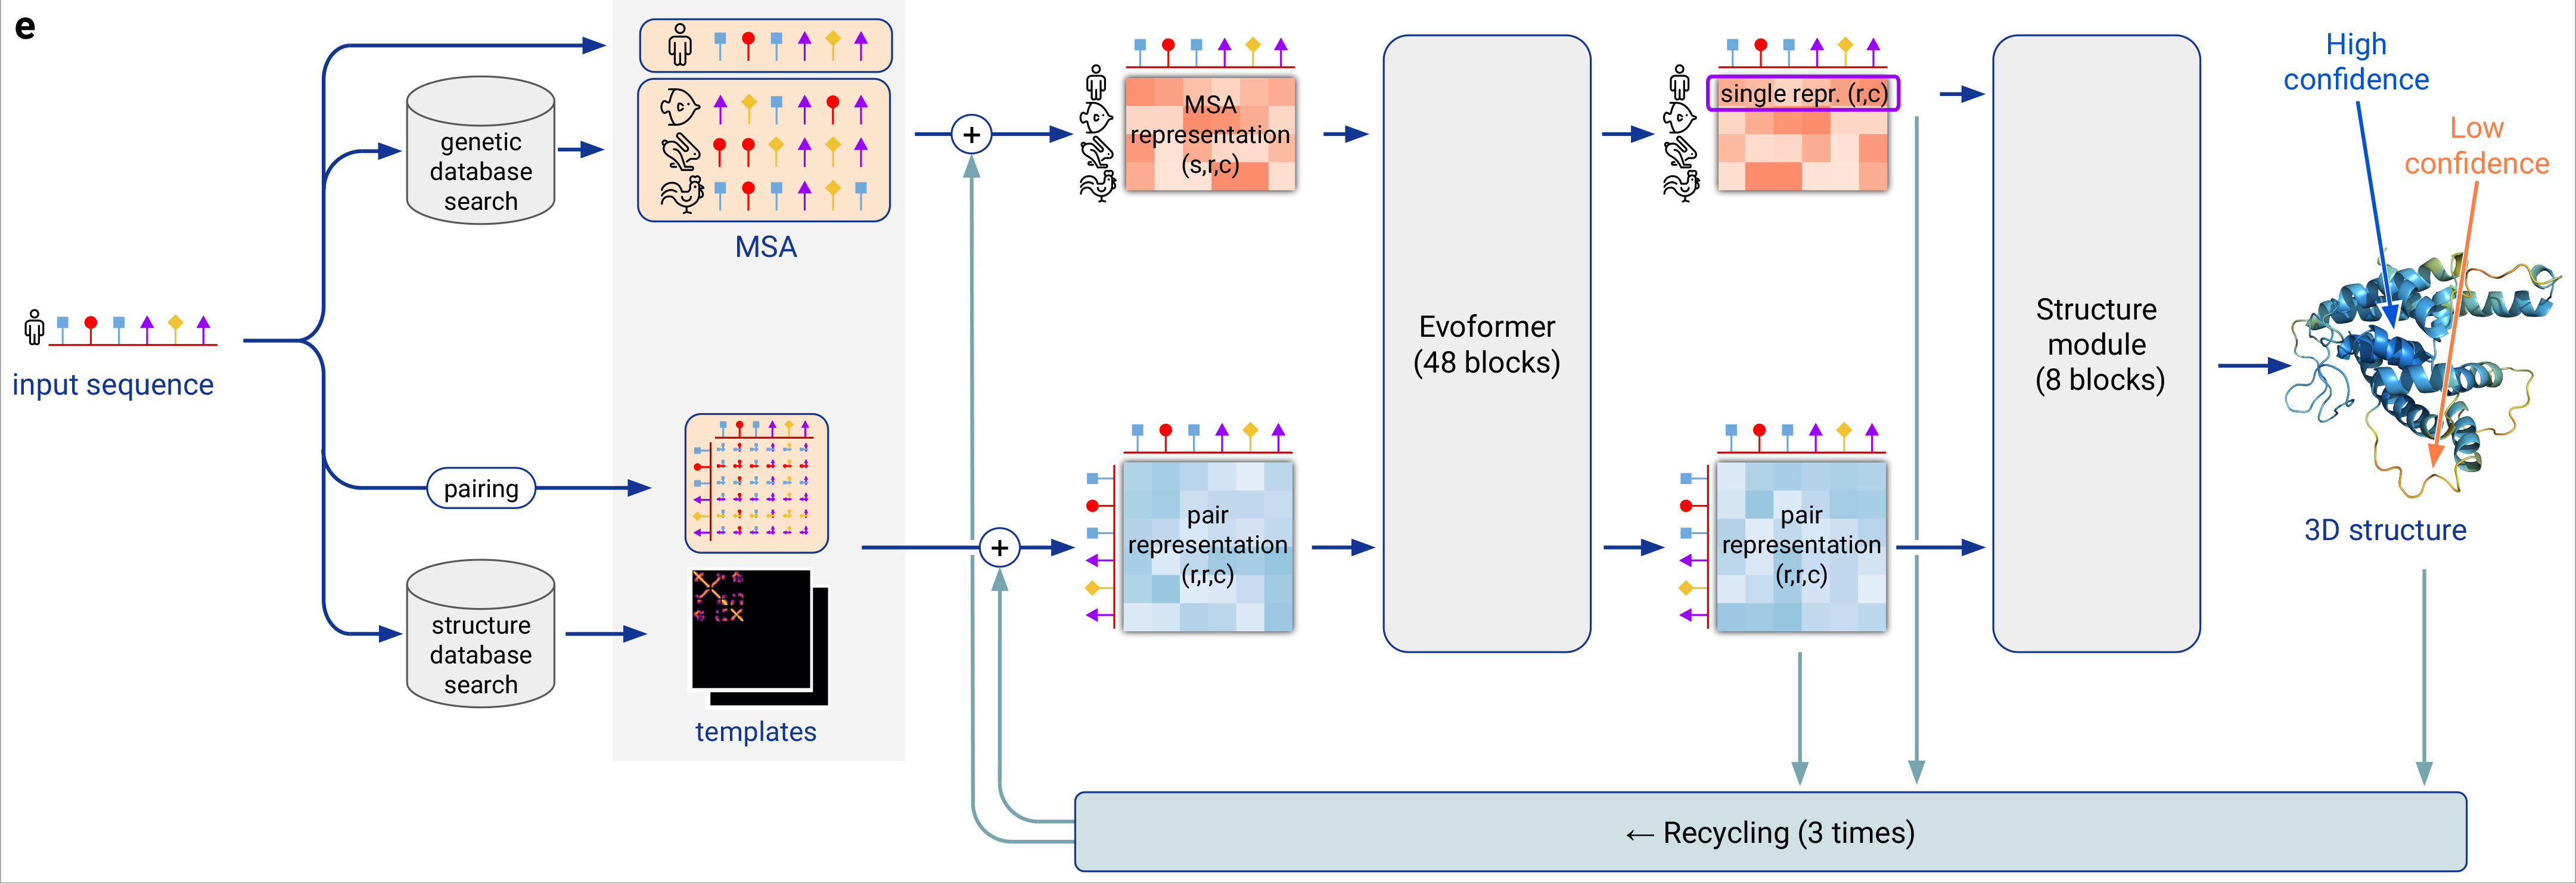
\includegraphics[width=.9\linewidth]{./imgs/model-overview.png}
\end{center} 
\end{frame}

\section*{Data Pipeline}
\label{sec:orgb8f4bae}
\begin{frame}[label={sec:orgd3b3cfa}]{Initial Input: mmCIF or FASTA files}
\begin{figure}[htbp]
\centering
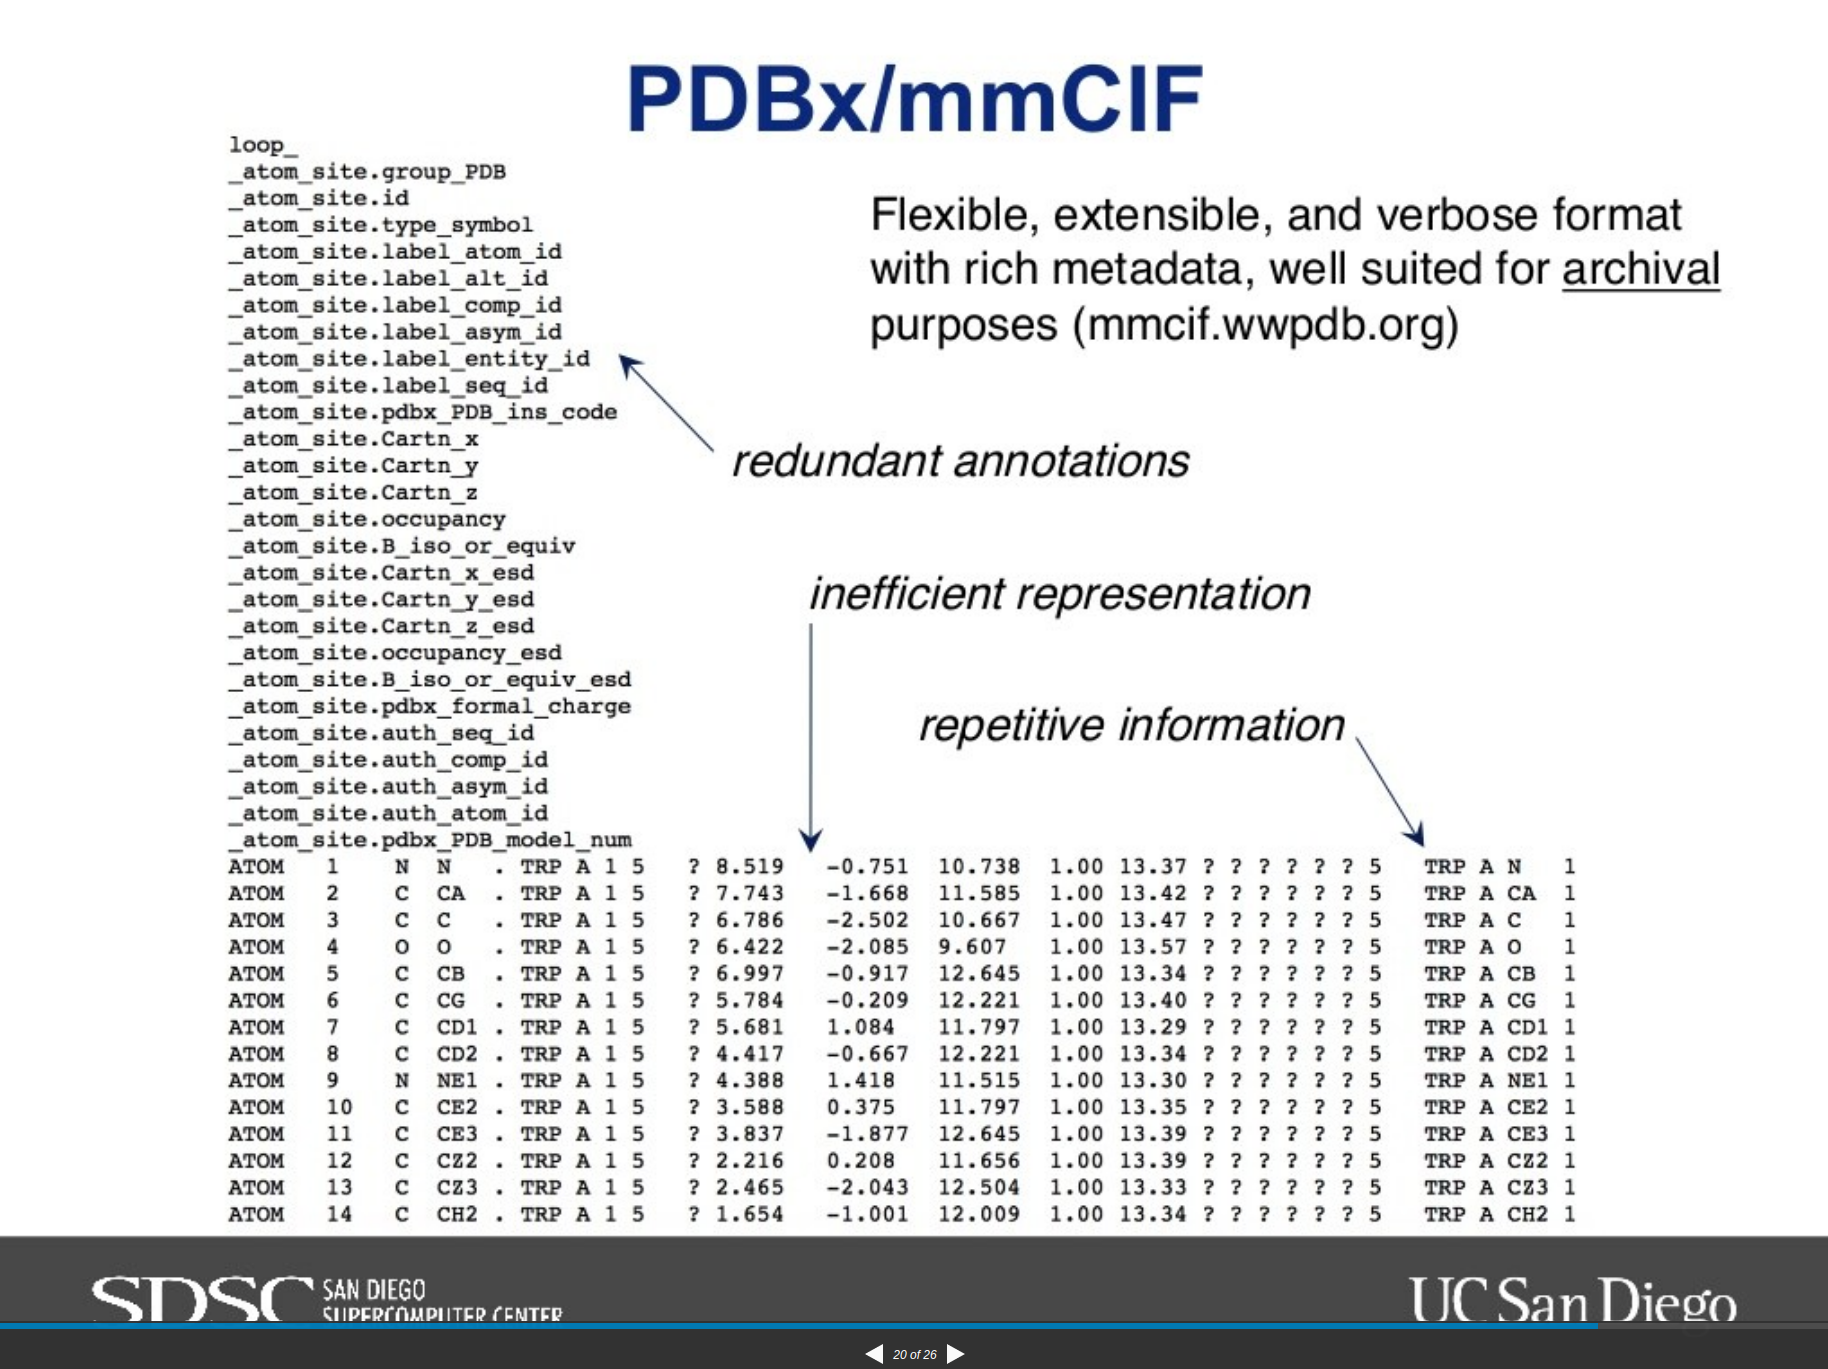
\includegraphics[height=0.8\textheight]{./imgs/mmcif-eg.png}
\caption{Example mmCIF file (see \protect\cite{PDB101LearnGuide})}
\end{figure}
\end{frame}


\begin{frame}[label={sec:org9fe96b5}]{Initial Input: mmCIF or FASTA files}
\begin{figure}[htbp]
\centering
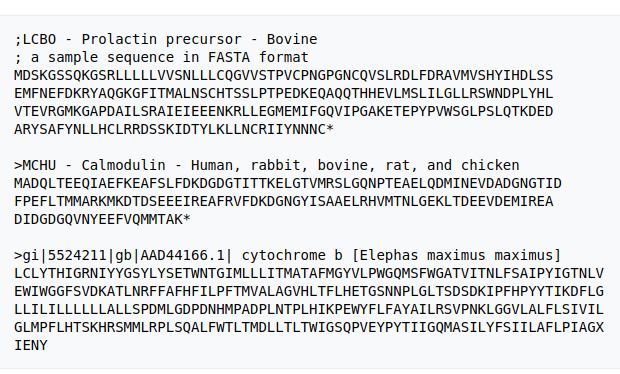
\includegraphics[width=.9\linewidth]{./imgs/fastafiles_2021-07-20.png}
\caption{Example FASTA file}
\end{figure}
\end{frame}

\begin{frame}[label={sec:orgab82f01}]{Parsing \cite{jumperHighlyAccurateProtein2021}}
\begin{itemize}
\item only certain metadata (more from mmCIF)
\item change MSE residues into MET
\end{itemize}
\end{frame}

\begin{frame}[label={sec:org7d4badc}]{Genetic Search \cite{jumperHighlyAccurateProtein2021}}
For MSAs
\begin{itemize}
\item JackHMMER
\begin{itemize}
\item MGnify: MSA depth 5,000
\item UniRef90: MSA depth 10,000
\end{itemize}
\item HHBlits
\begin{itemize}
\item Uniclust30 + BFD: MSA depth unlimited
\end{itemize}
\item MSAs duplicated and stacked
\end{itemize}

\begin{quote}
flags: \\
  JackHMMER: -N 1 -E 0.0001 --incE 0.0001 --F1 0.0005 --F2 0.00005 --F3 0.0000005. \\
  HHBlits: -n 3 -e 0.001 -realign\textsubscript{max} 100000 -maxfilt 100000 -min\textsubscript{prefilter}\textsubscript{hits} 1000 -maxseq 1000000.
\end{quote}
\end{frame}

\begin{frame}[label={sec:orge7ae846}]{Template Search \cite{jumperHighlyAccurateProtein2021}}
\begin{itemize}
\item UniRef90 MSA from prior search used for PDB70 search using HHSearch.
\item Filter out:
\begin{itemize}
\item released after the input sequence
\item or identical to the input sequence
\item too small
\end{itemize}
\item At inference use top 4 templates
\end{itemize}
\end{frame}

\begin{frame}[label={sec:orge857553}]{Training Data \cite{jumperHighlyAccurateProtein2021}}
\begin{itemize}
\item 75:25 self-distillation : known structure (PDB)
\item stochastic filters (next)
\end{itemize}
\end{frame}

\begin{frame}[label={sec:org433cc0a}]{Filtering \cite{jumperHighlyAccurateProtein2021}}
\begin{itemize}
\item stochastic filters: 
\begin{itemize}
\item Input mmCIFs are restricted to have resolution less than 9 Å. This is not a very restrictive filter and only removes around 0.2\% of structures.
\item Longer protein chains are selected with higher probability.
\item Also favour protein chains from smaller clusters. They use 40\% sequence identity clusters of the Protein Data Bank clustered with MMSeqs2.
\item Sequences are filtered out when any single amino acid accounts for more than 80\% of the input primary sequence. This filter removes about 0.8\% of sequences.
\end{itemize}
\end{itemize}
\end{frame}

\begin{frame}[label={sec:org0207119}]{MSA block deletion \cite{jumperHighlyAccurateProtein2021}}
\begin{itemize}
\item Block deletion tends to remove similarities (ie. whole branch phylogeny) and promote diversity
\begin{itemize}
\item Similar sequences are likely to be adjacent
\item Contiguous blocks in MSAs are deleted.
\item First MSAs are grouped by tool
\item Then sorted according to tool defaults (usually e-value)
\end{itemize}
\end{itemize}
\end{frame}

\begin{frame}[label={sec:orgc02b307}]{Algorithm 1 MSA Block deletion \cite{jumperHighlyAccurateProtein2021}}
\begin{center}
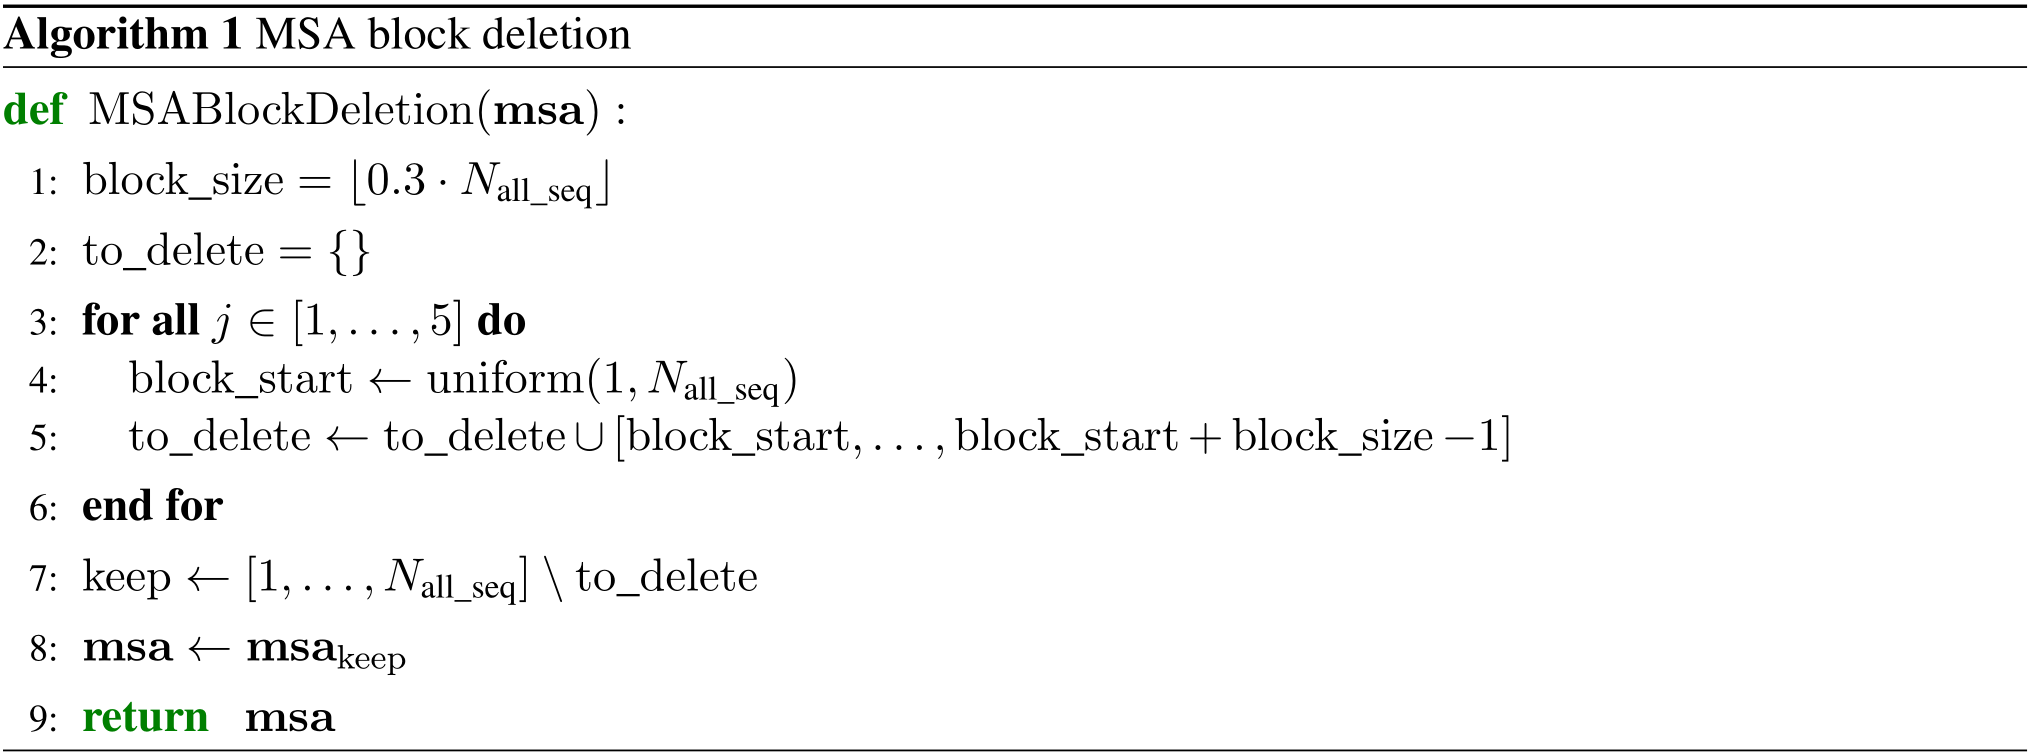
\includegraphics[width=.9\linewidth]{./imgs/algo1_block_deletion.png}
\end{center}
\end{frame}
\begin{frame}[label={sec:orgca76dd1}]{MSA clustering \cite{jumperHighlyAccurateProtein2021}}
\begin{itemize}
\item Similarity clusters used to randomly select subset of MSA sequences 
\begin{itemize}
\item to reduce computational cost from attention modules, reduce \(N_seq\)
\end{itemize}
\item Modified K-means is used, with the input sequence used as first cluster center
\end{itemize}

Clustering Algorithm:
\begin{enumerate}
\item \(N_{clust}\) centers selected from MSA
\item Generate a mask where \emph{p=0.15} that any position is selected by the mask
\item Each center is modified for each mask selected residue according to:
\begin{enumerate}
\item \emph{p=0.1} replaced with a uniformly sampled random amino acid
\item \emph{p=0.1} replaced with an amino acid sampled from the MSA profile
\item \emph{p=0.1} no replacement
\item \emph{p=0.7} replaced with a special token (masked\textsubscript{msa}\textsubscript{token})
\end{enumerate}
\item hamming distance measure for remaining selections
\end{enumerate}
\end{frame}

\begin{frame}[label={sec:orgc5d6117}]{Residue cropping \cite{jumperHighlyAccurateProtein2021}}
During training:
\begin{enumerate}
\item unclamped \& clamped - sampling start index from uniform distributions
\item Cropped with fixed size \(N_res\)
\end{enumerate}
\end{frame}

\begin{frame}[label={sec:orgc1cec96}]{Featurization and model inputs \cite{jumperHighlyAccurateProtein2021}}
\begin{itemize}
\item \alert{target\textsubscript{feat}} \\
This is a feature of size [Nres, 21] consisting of the “aatype” feature.
\item \alert{residue\textsubscript{index}} \\
Positional encoding constant tensor. This is a feature of size [Nres] consisting of the “residue\textsubscript{index}” feature.
\item \alert{msa\textsubscript{feat}} \\
This is a feature of size [Nclust, Nres, 49] constructed by concatenating “cluster\textsubscript{msa}”, “cluster\textsubscript{has}\textsubscript{deletion}”, “cluster\textsubscript{deletion}\textsubscript{value}”, “cluster\textsubscript{deletion}\textsubscript{mean}”, “cluster\textsubscript{profile}”. We draw Ncycle×Nensemble random samples from this feature to provide each recycling/ensembling iteration of the network with a different sample (see subsubsection 1.11.2).
\item \alert{extra\textsubscript{msa}\textsubscript{feat}} \\
This is a feature of size [Nextra\textsubscript{seq}, Nres, 25] constructed by concatenating “extra\textsubscript{msa}”, “extra\textsubscript{msa}\textsubscript{has}\textsubscript{deletion}”, “extra\textsubscript{msa}\textsubscript{deletion}\textsubscript{value}”. Together with “msa\textsubscript{feat}’ above we also draw Ncycle × Nensemble random samples from this feature (see subsubsection 1.11.2).
\end{itemize}
\end{frame}
\begin{frame}[label={sec:org6352966}]{Featurization and model inputs \cite{jumperHighlyAccurateProtein2021}}
\begin{itemize}
\item \alert{template\textsubscript{pair}\textsubscript{feat}} \\
This is a feature of size [Ntempl, Nres, Nres, 88] and consists of concatenation of the pair residue features “template\textsubscript{distogram}”, “template\textsubscript{unit}\textsubscript{vector}”, and also several residue features, which are transformed into pair features. \\
The “template\textsubscript{aatype}” feature is included via tiling and stacking (this is done twice, in both residue directions). \\
Also the mask features “template\textsubscript{pseudo}\textsubscript{beta}\textsubscript{mask}” and “template\textsubscript{backbone}\textsubscript{frame}\textsubscript{mask}” are included, where the feature fij = maski · maskj. \\
\item \alert{template\textsubscript{angle}\textsubscript{feat}} \\
This is a feature of size [Ntempl, Nres, 51] constructed by concatenating the following features: “template\textsubscript{aatype}”, “template\textsubscript{torsion}\textsubscript{angles}”, “template\textsubscript{alt}\textsubscript{torsion}\textsubscript{angles}”, and “template\textsubscript{torsion}\textsubscript{angles}\textsubscript{mask}”.
\end{itemize}
\end{frame}

\begin{frame}[label={sec:orgf17f0ea}]{Table 1 Input Features (1/2) \cite{jumperHighlyAccurateProtein2021}}
\begin{center}
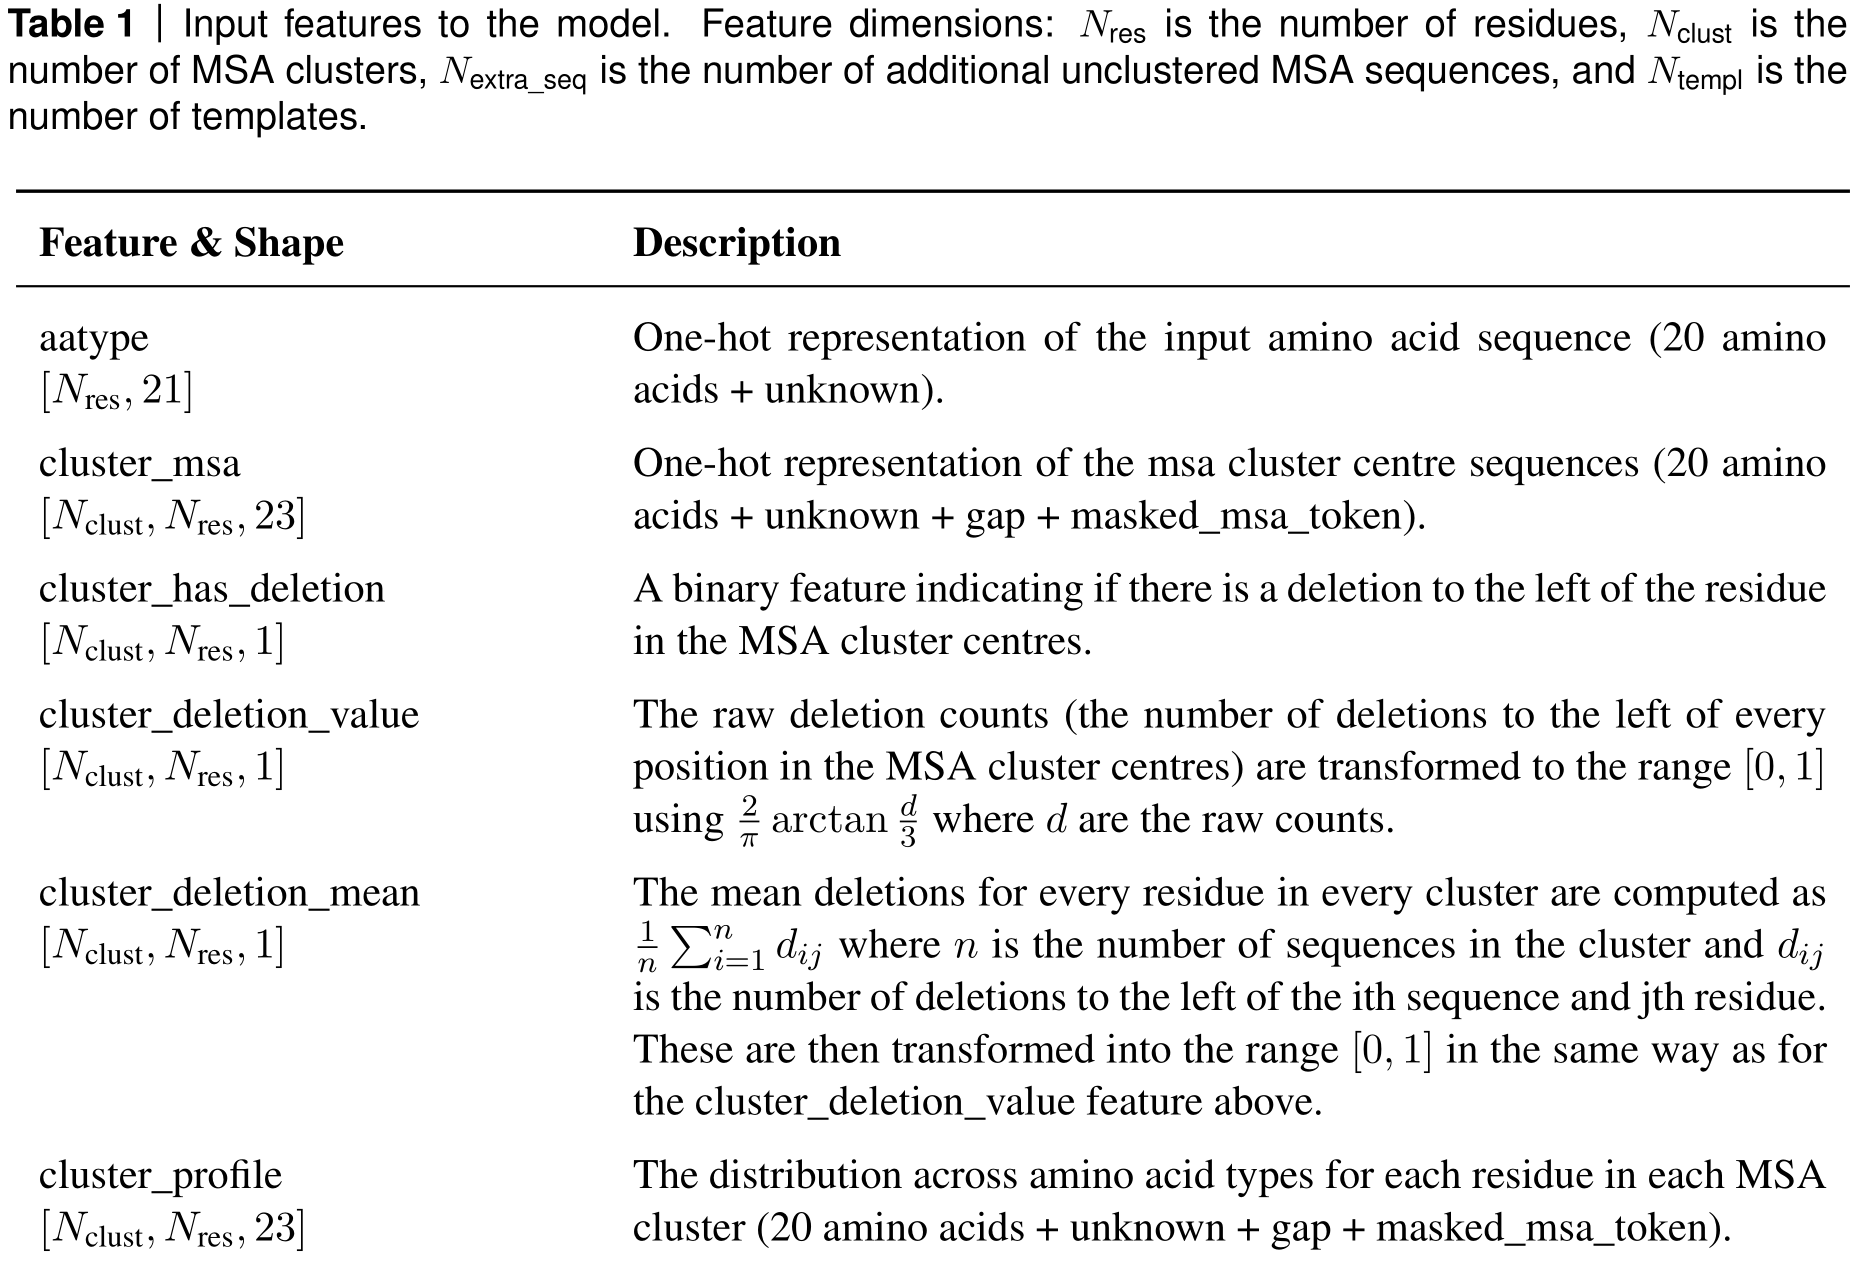
\includegraphics[height=0.8\textheight]{./imgs/table1_inputs_1.png}
\end{center}
\end{frame}
\begin{frame}[label={sec:orgacca343}]{Table 1 Input Features (2/2) \cite{jumperHighlyAccurateProtein2021}}
\begin{center}
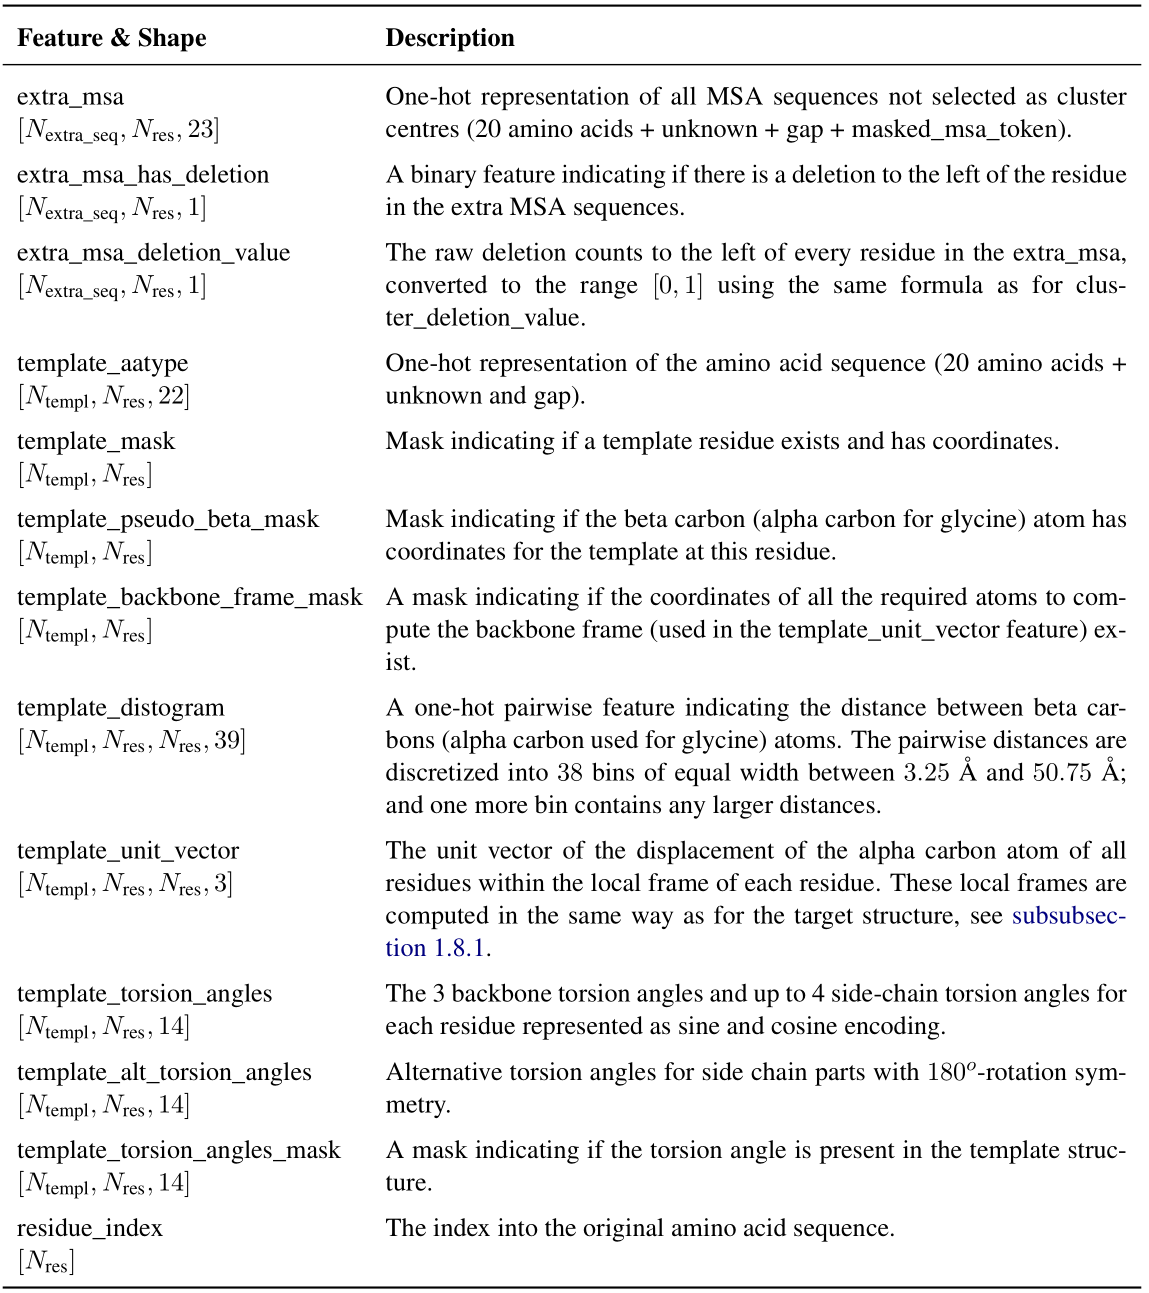
\includegraphics[height=0.8\textheight]{./imgs/table1_inputs_2.png}
\end{center}
\end{frame}

\begin{frame}[label={sec:orga51b4f4}]{Self-distillation dataset \cite{jumperHighlyAccurateProtein2021}}
\begin{itemize}
\item Build dataset (on unlabeled sequences):
\begin{enumerate}
\item Make MSA for every cluster in Uniclust30
\item Remove sequences that appear in another sequences MSA
\item Keep sequences of 200 < length < 1024
\item Remove sequences where MSA < 200 alignments
\end{enumerate}
\item For predicted structures:
\begin{itemize}
\item train 'undistlled' model on just PDB dataset
\item use this model to predict above set
\item for every residue pair, computer confidence metric using KL-divergence between distance distribution and a reference distribution
\item reference distribution
\end{itemize}
\item self-distillation training took roughly 2 weeks
\end{itemize}
\end{frame}

\section*{AlphaFold Inference}
\label{sec:orgb517554}
\begin{frame}[label={sec:org47c1339}]{AlphaFold Inference \cite{jumperHighlyAccurateProtein2021}}
\begin{itemize}
\item AlphaFold receives input features derived from:
\begin{itemize}
\item the amino-acid sequence
\item MSA
\item templates (see subsubsection 1.2.9)
\end{itemize}
\item outputs features:
\begin{itemize}
\item atom coordinates
\item the distogram
\item per-residue confidence scores.
\end{itemize}
\item Recycling x3
\begin{itemize}
\item initial recycled inputs are zero
\end{itemize}
\end{itemize}

Algorithm 2 outlines the main steps (see also Fig 1e and the corresponding description in the main article).
\end{frame}

\begin{frame}[label={sec:orgc8b034f}]{Algorithm 2 Model Inference \cite{jumperHighlyAccurateProtein2021}}
\begin{center}
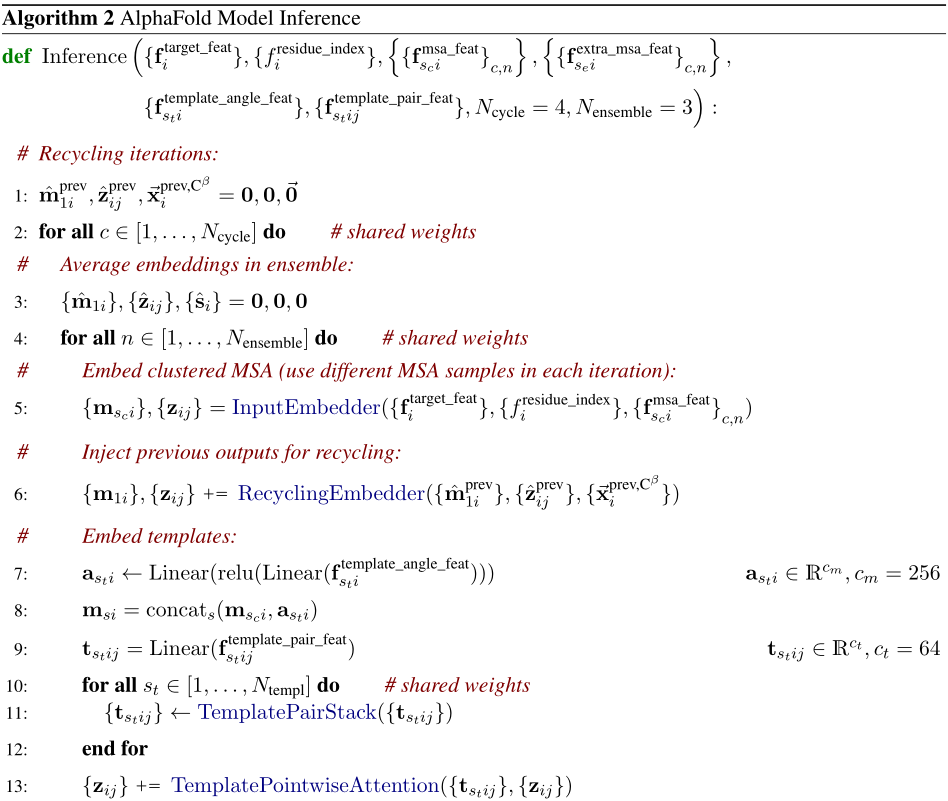
\includegraphics[height=0.9\textheight]{./imgs/algo2_cut_part1.png}
\end{center}
\end{frame}
\begin{frame}[label={sec:org7527166}]{Algorithm 2 Model Inference \cite{jumperHighlyAccurateProtein2021}}
\begin{center}
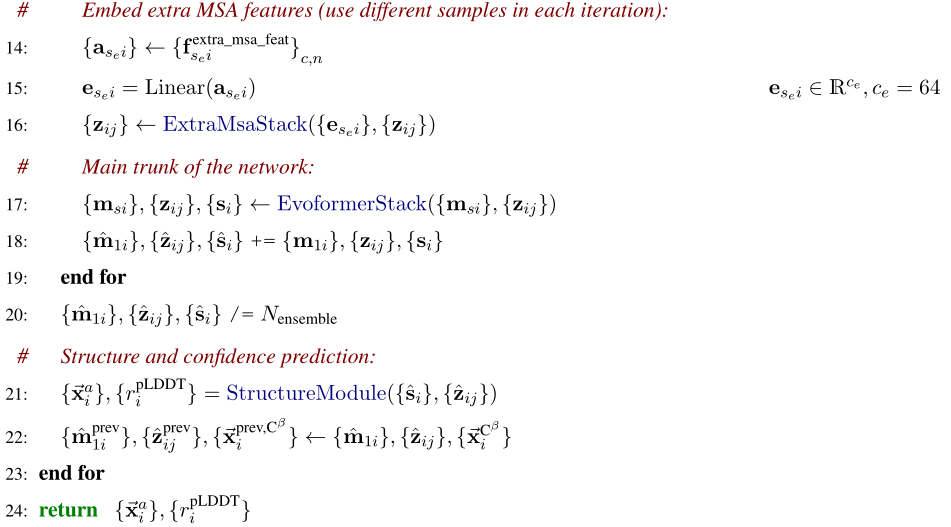
\includegraphics[height=0.9\textheight]{./imgs/algo2_cut_part2.png}
\end{center}
\end{frame}
\begin{frame}[label={sec:org039c15e}]{AlphaFold Training \cite{jumperHighlyAccurateProtein2021}}
\begin{center}
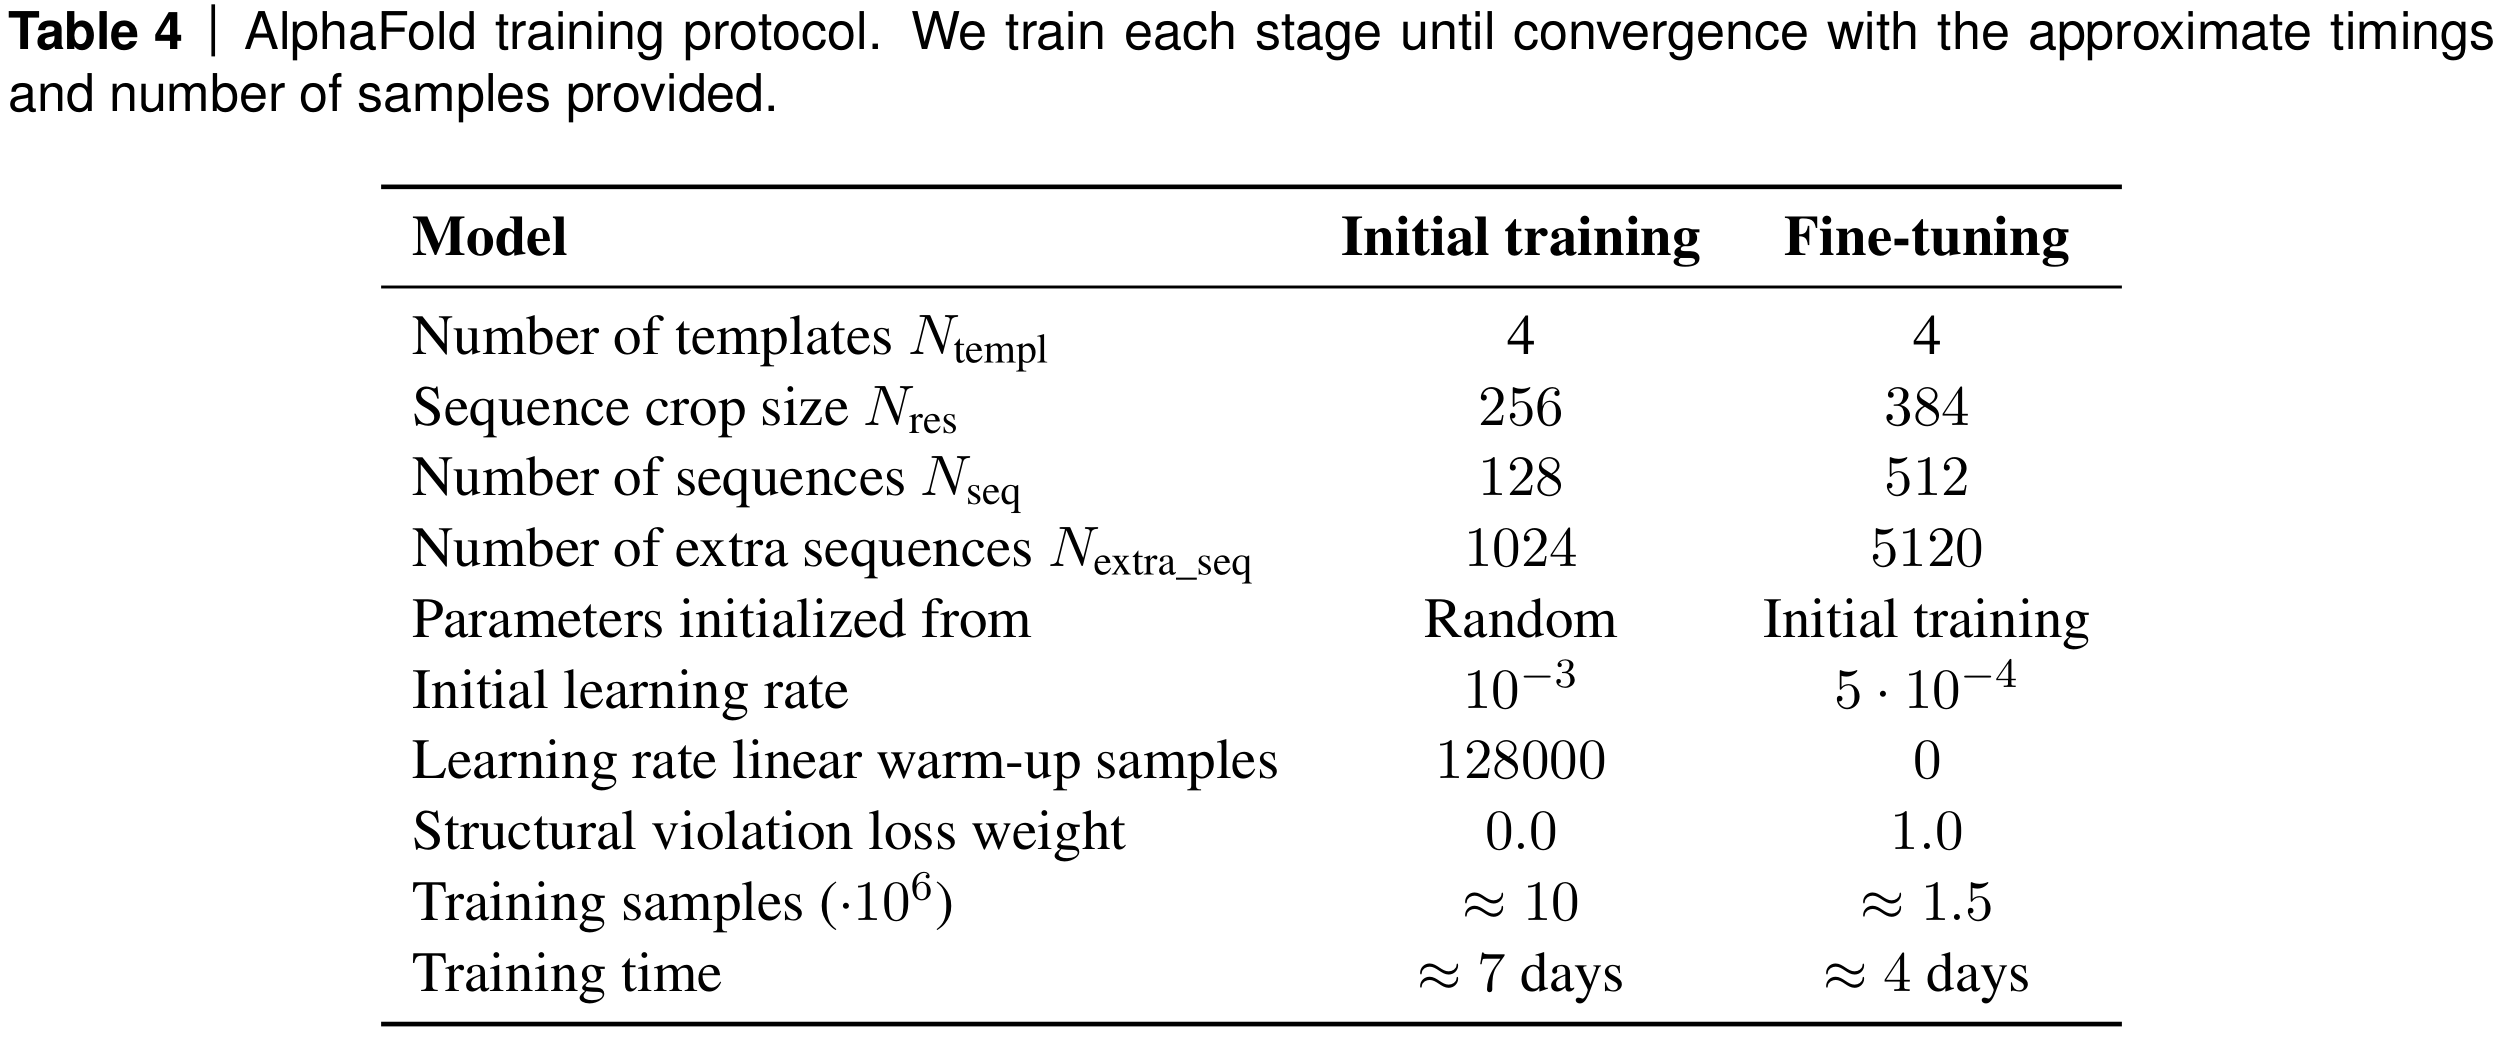
\includegraphics[width=.9\linewidth]{./imgs/table4_model_training.png}
\end{center}
\end{frame}
\section*{Model Architecture}
\label{sec:org899b221}
\begin{frame}[label={sec:org8dffce4}]{Input embeddings \cite{jumperHighlyAccurateProtein2021}}
\begin{center}
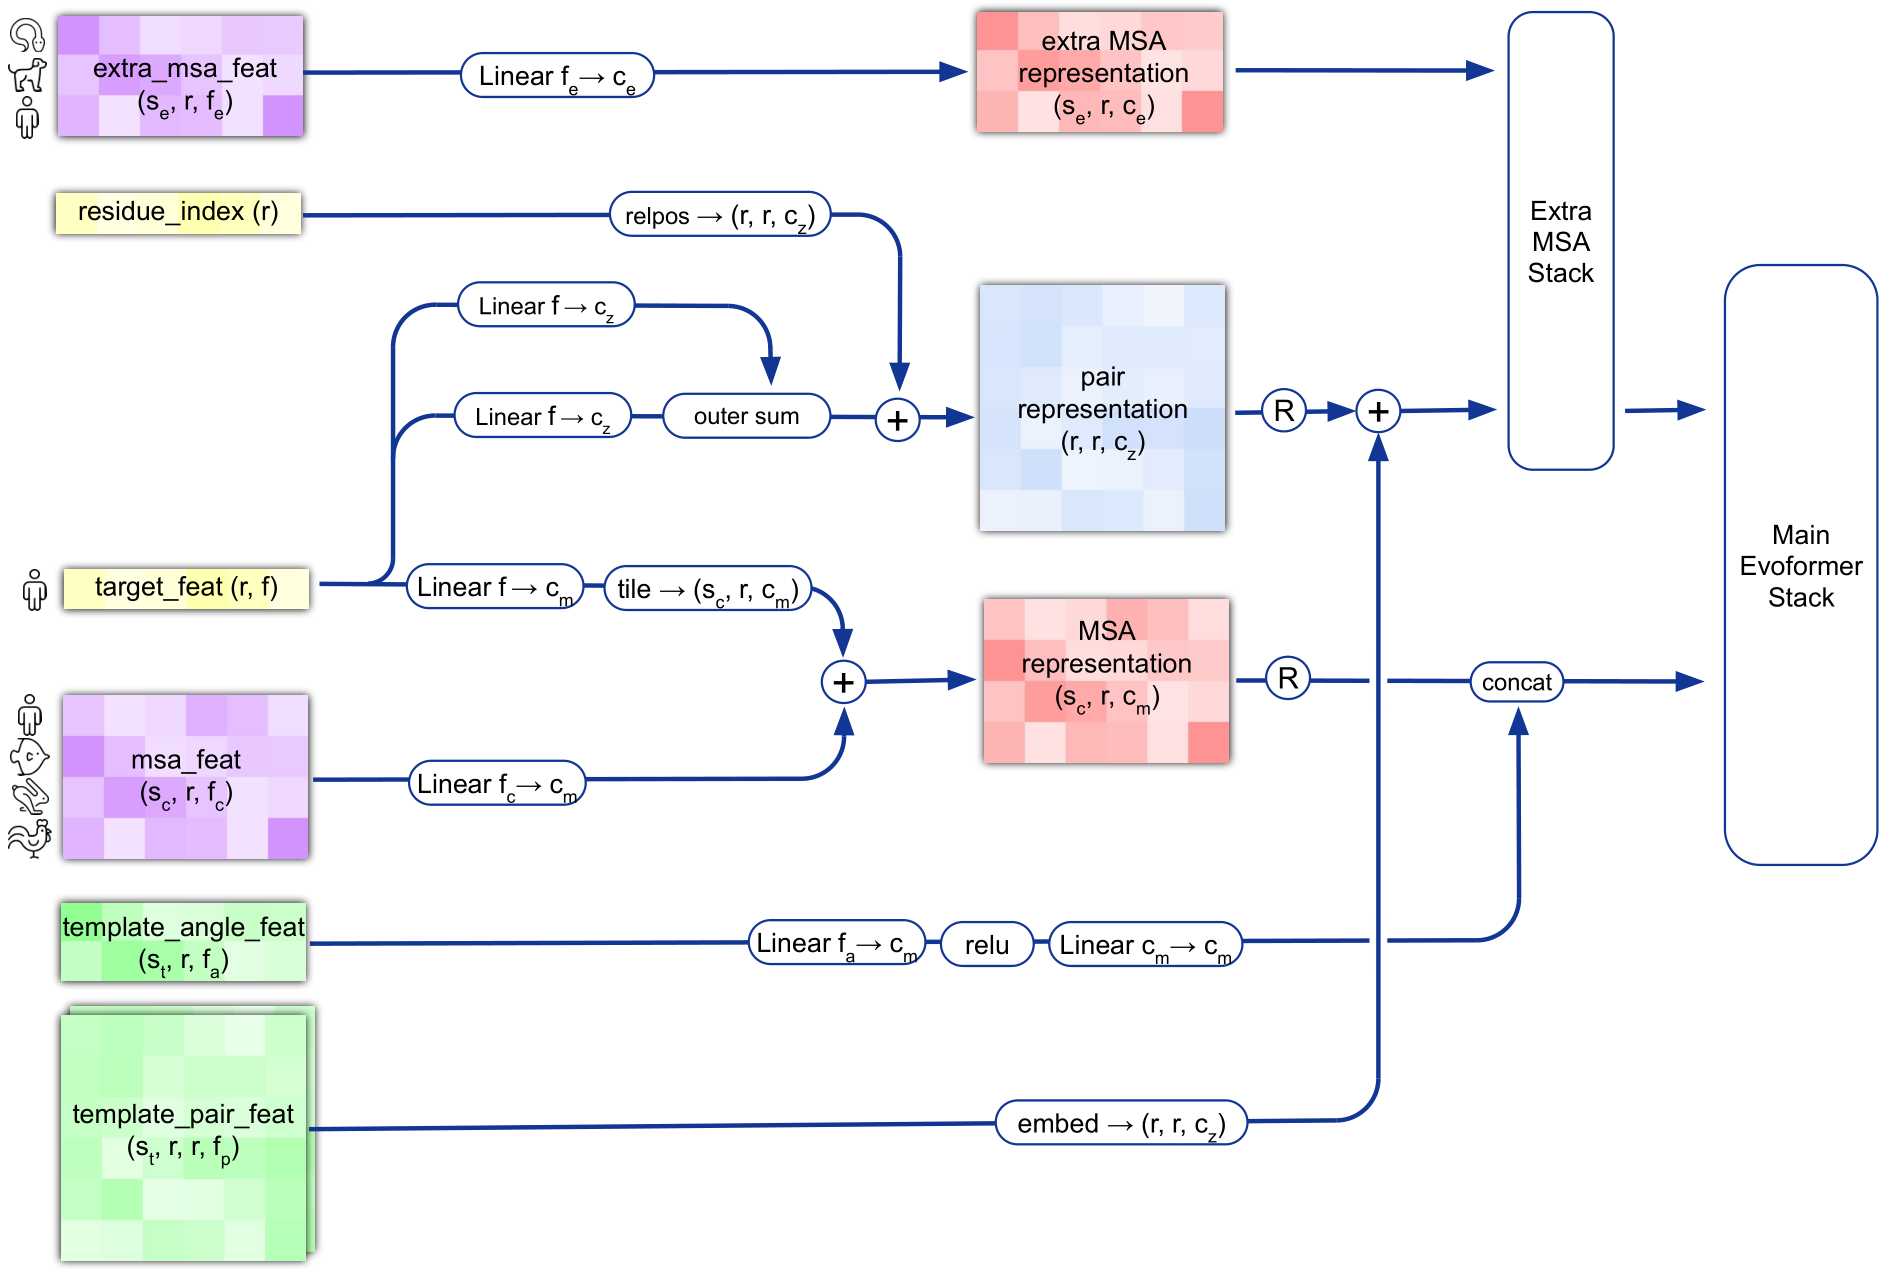
\includegraphics[height=0.9\textheight]{./imgs/input_embeddings.png}
\end{center}
\end{frame}
\begin{frame}[label={sec:org46e8194}]{Algorithm 3 Input embeddings \cite{jumperHighlyAccurateProtein2021}}
\begin{center}
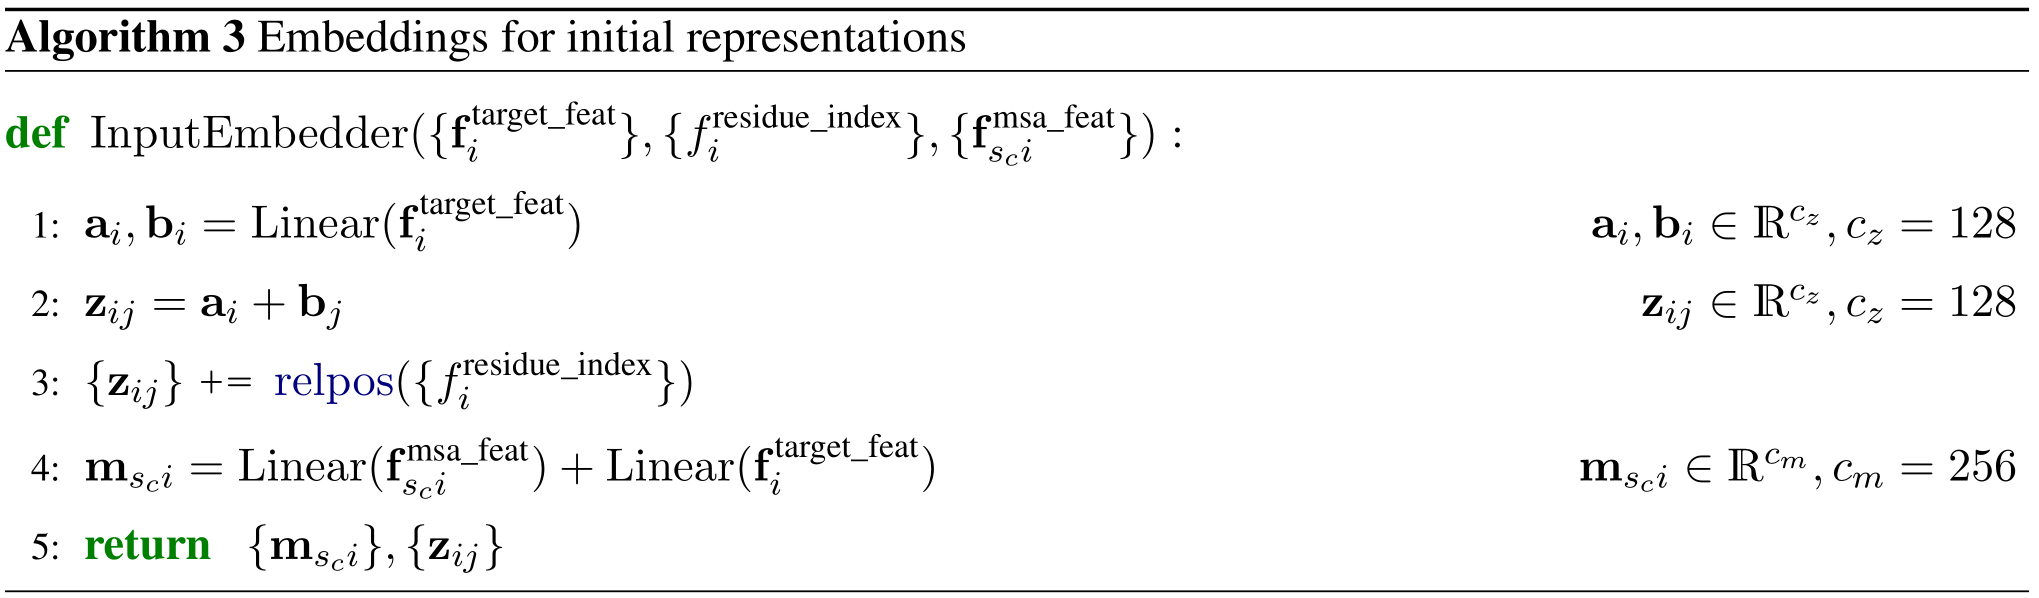
\includegraphics[width=.9\linewidth]{./imgs/algo3_input_embed.png}
\end{center}
\end{frame}
\begin{frame}[label={sec:org4b52f64}]{Algorithm 4 Relative positional encoding \cite{jumperHighlyAccurateProtein2021}}
\begin{center}
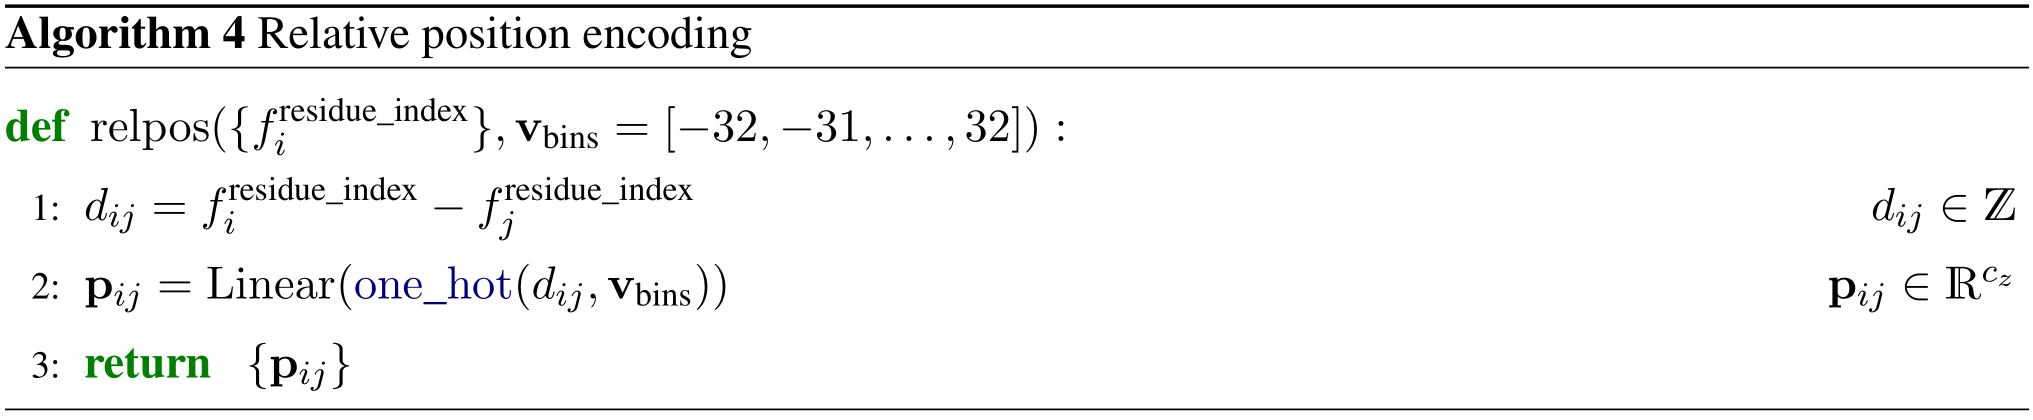
\includegraphics[width=.9\linewidth]{./imgs/algo4_pos_encoding.png}
\end{center}
\end{frame}
\begin{frame}[label={sec:org8924895}]{Algorithm 5 One-hot encoding with nearest bin \cite{jumperHighlyAccurateProtein2021}}
\begin{center}
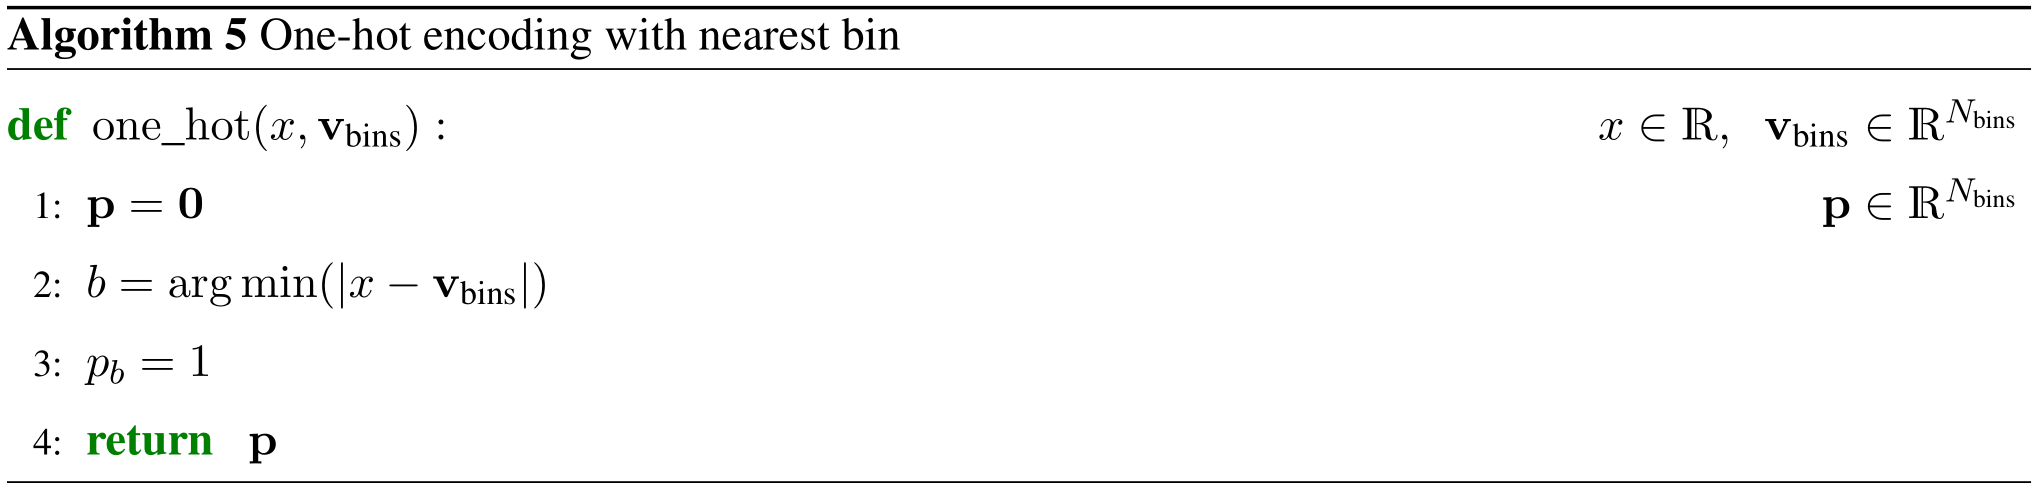
\includegraphics[width=.9\linewidth]{./imgs/algo5_1hot_bin_encode.png}
\end{center}
\end{frame}

\subsection*{EvoFormer}
\label{sec:org73915f7}
\begin{frame}[label={sec:org439ec00}]{EvoFormer: Overview \cite{jumperHighlyAccurateProtein2021}}
\begin{center}
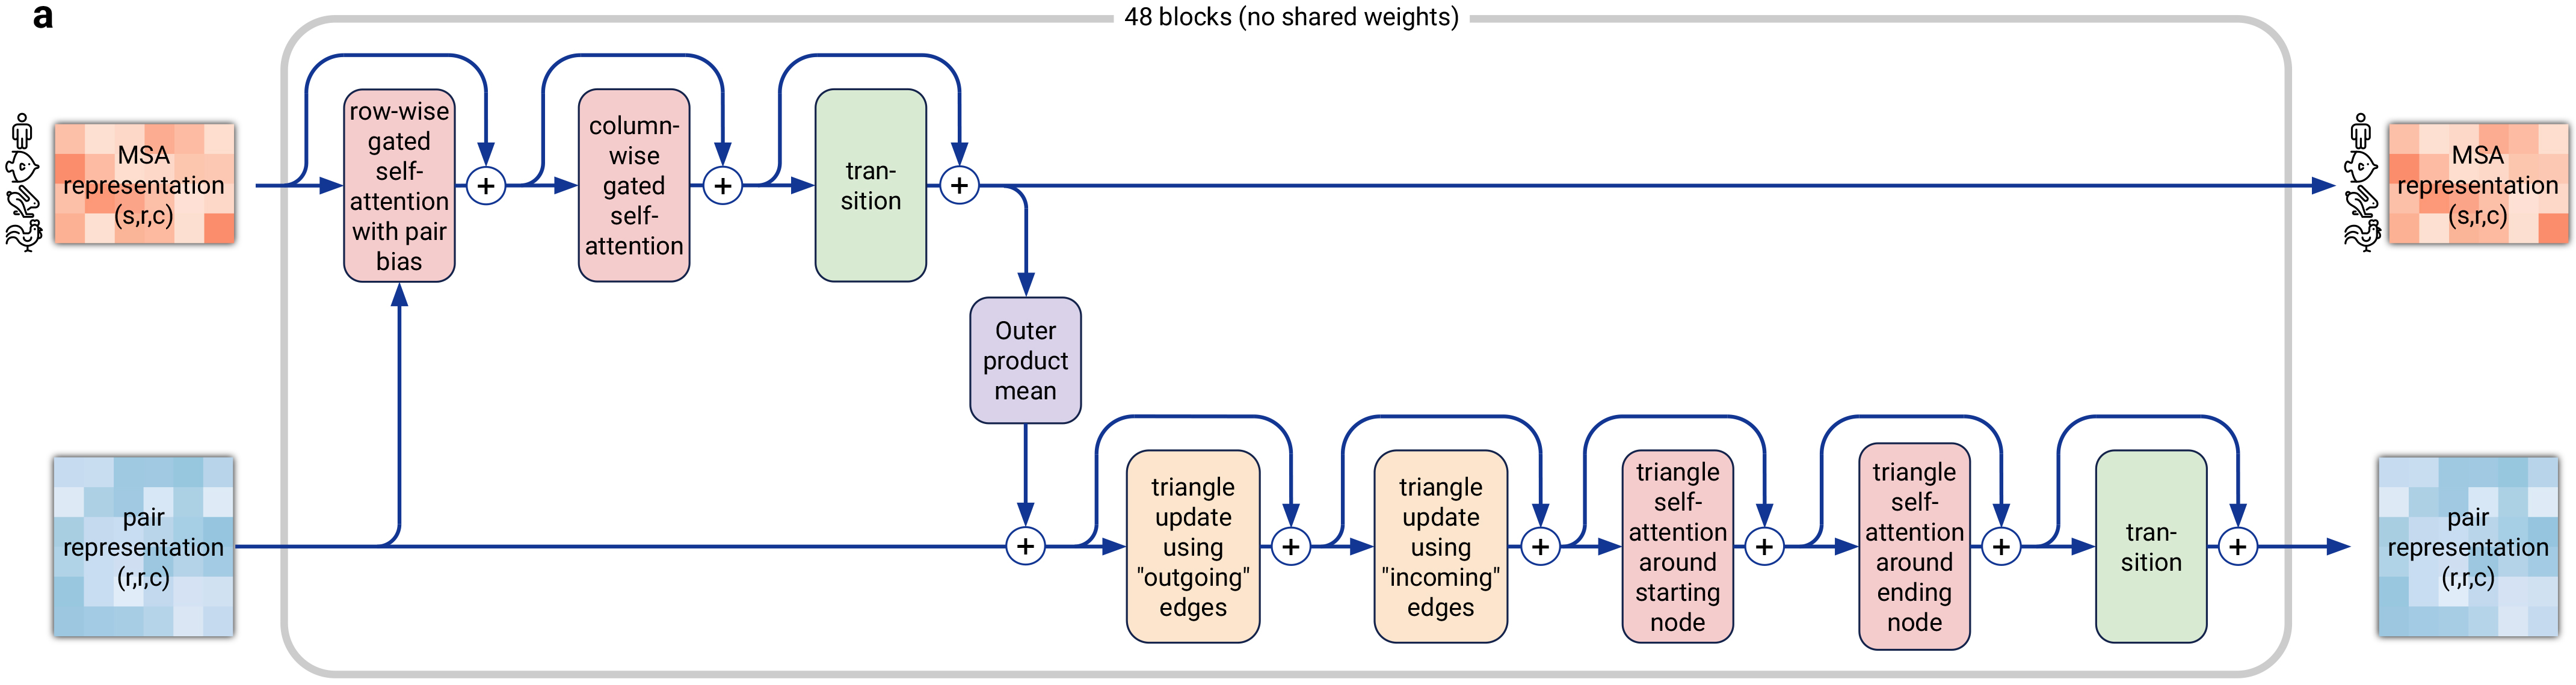
\includegraphics[width=.9\linewidth]{./imgs/model-evoformer-main.png}
\end{center} 
\end{frame}

\begin{frame}[label={sec:org8d34d0c}]{EvoFormer: Overview \cite{jumperHighlyAccurateProtein2021}}
\begin{itemize}
\item cast as a graph inference problem
\item cross-optimization and information flow between MSA representation and pair-wise representation
\item layer normalization
\end{itemize}
\end{frame}
\begin{frame}[label={sec:org877b8c2}]{Algorithm 6 EvoFormer stack \cite{jumperHighlyAccurateProtein2021}}
\begin{center}
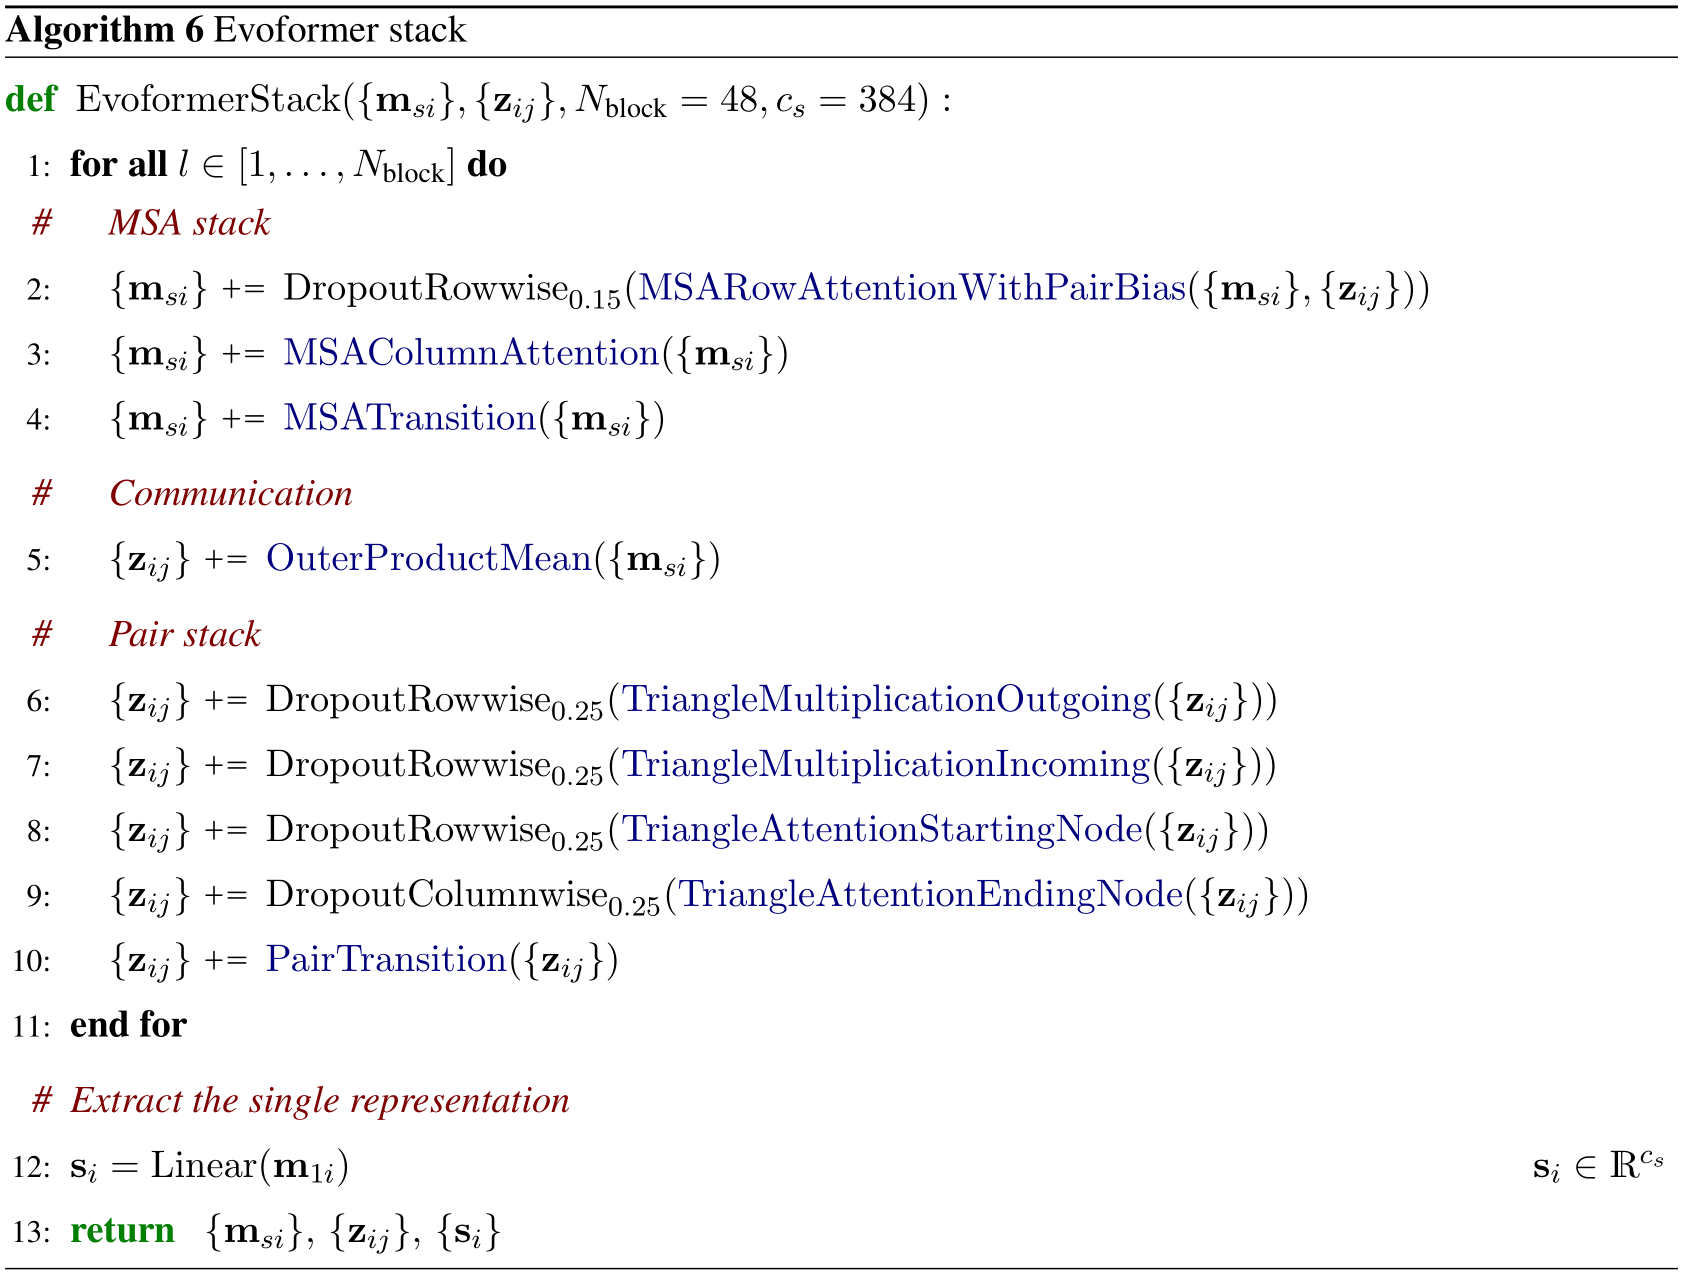
\includegraphics[height=0.9\textheight]{./imgs/algo6_evoformer.png}
\end{center}
\end{frame}

\begin{frame}[label={sec:org65e915b}]{EvoFormer: Row wise Gated Attention \cite{jumperHighlyAccurateProtein2021}}
\begin{center}
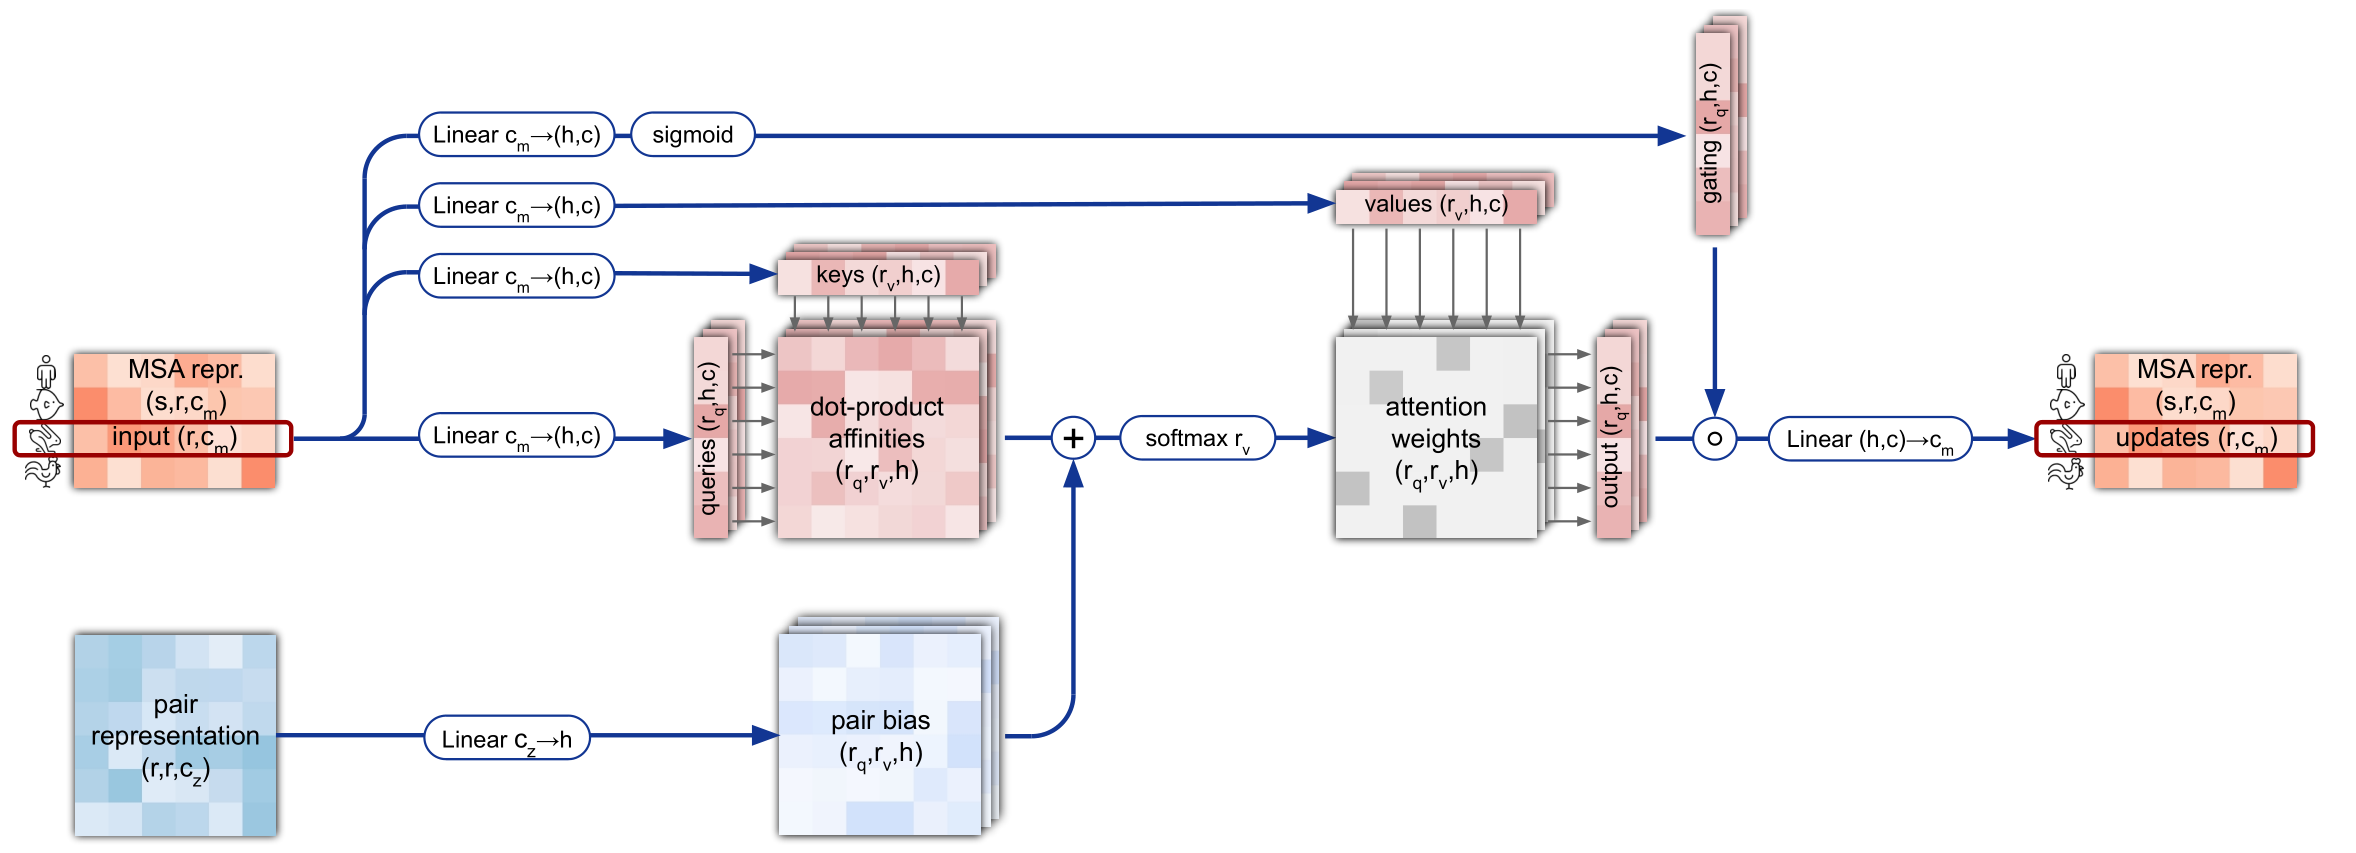
\includegraphics[width=.9\linewidth]{./imgs/rowwise-gated-attention.png}
\end{center}
\end{frame}

\begin{frame}[label={sec:orgaf15a10}]{Algorithm 7 Row wise Gated Attention \cite{jumperHighlyAccurateProtein2021}}
\begin{center}
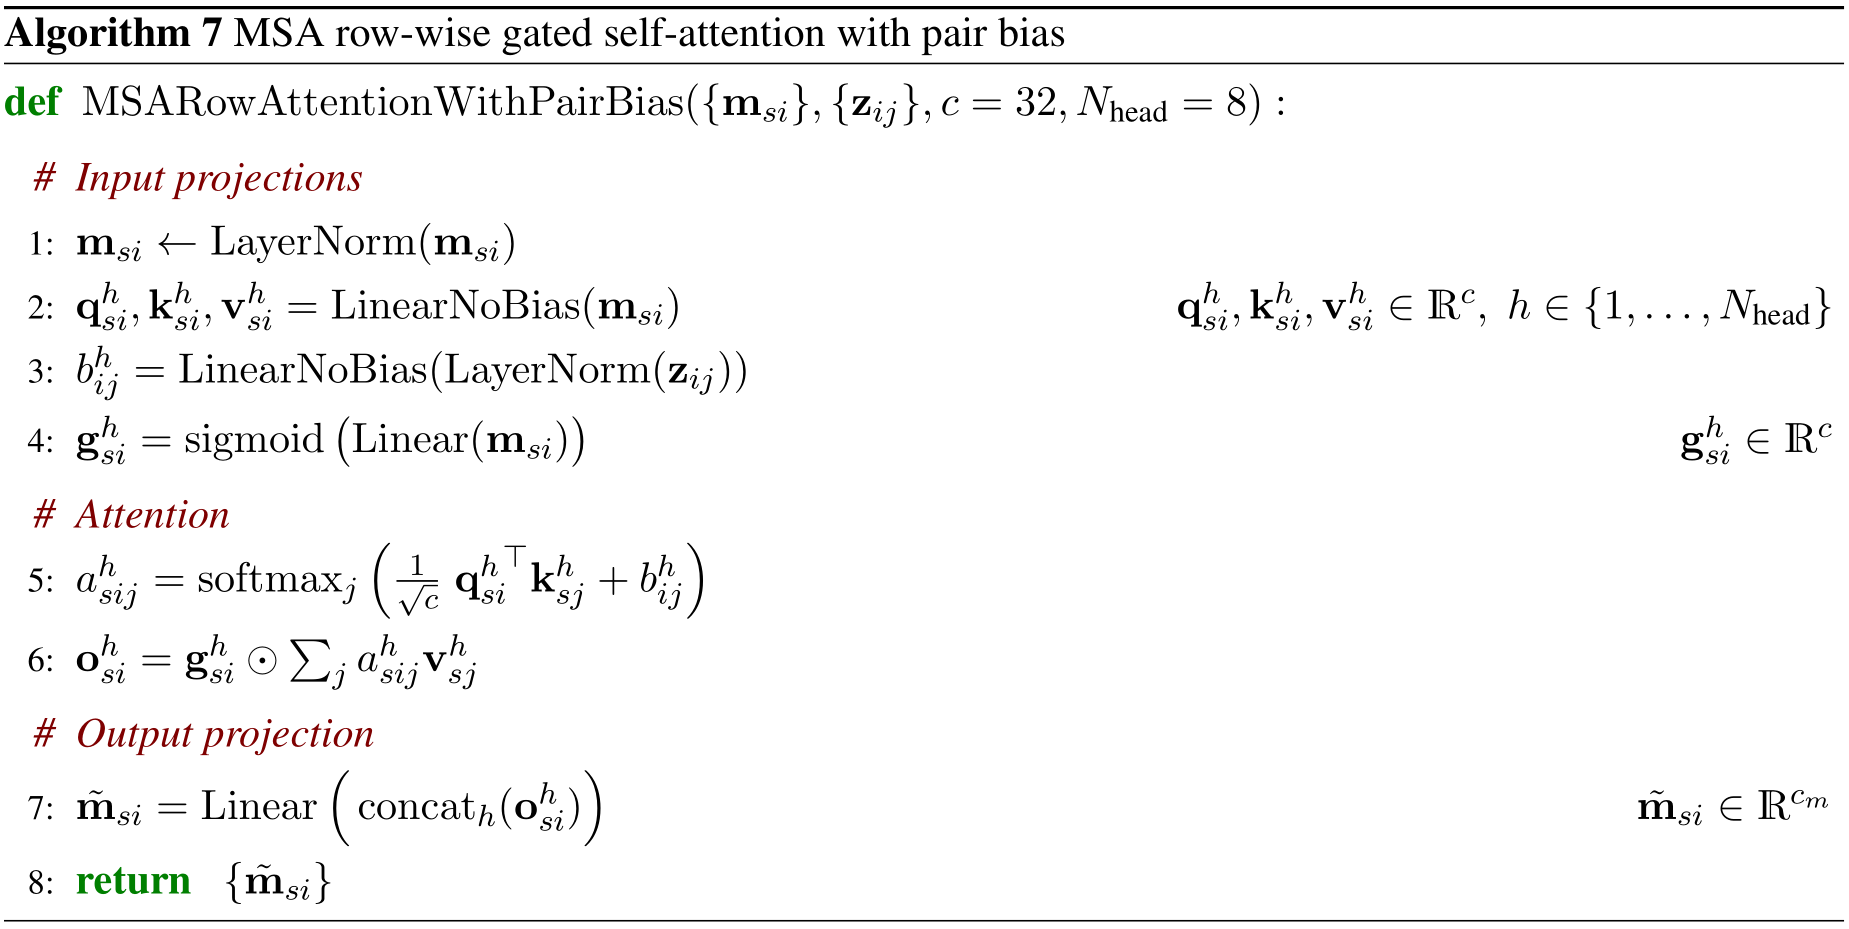
\includegraphics[height=0.8\textheight]{./imgs/algo7_evo_row_attention.png}
\end{center}
\end{frame}

\begin{frame}[label={sec:orgf5d6a96}]{EvoFormer: Column wise Gated Attention \cite{jumperHighlyAccurateProtein2021}}
\begin{center}
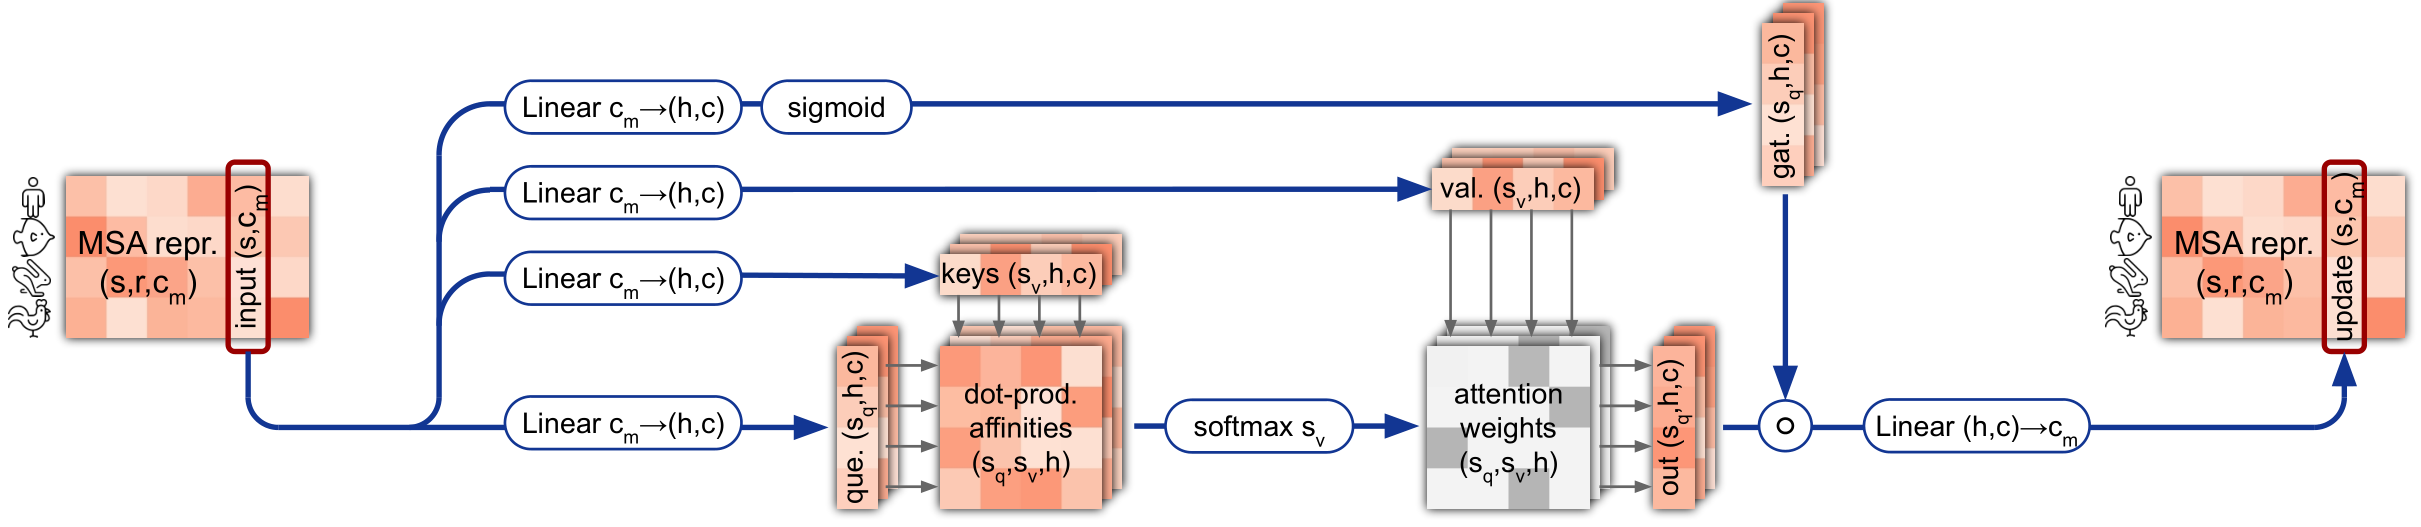
\includegraphics[width=.9\linewidth]{./imgs/columnwise-gated-attention.png}
\end{center}
\end{frame}

\begin{frame}[label={sec:org4e9c184}]{Algorithm 8 Column wise Gated Attention \cite{jumperHighlyAccurateProtein2021}}
\begin{center}
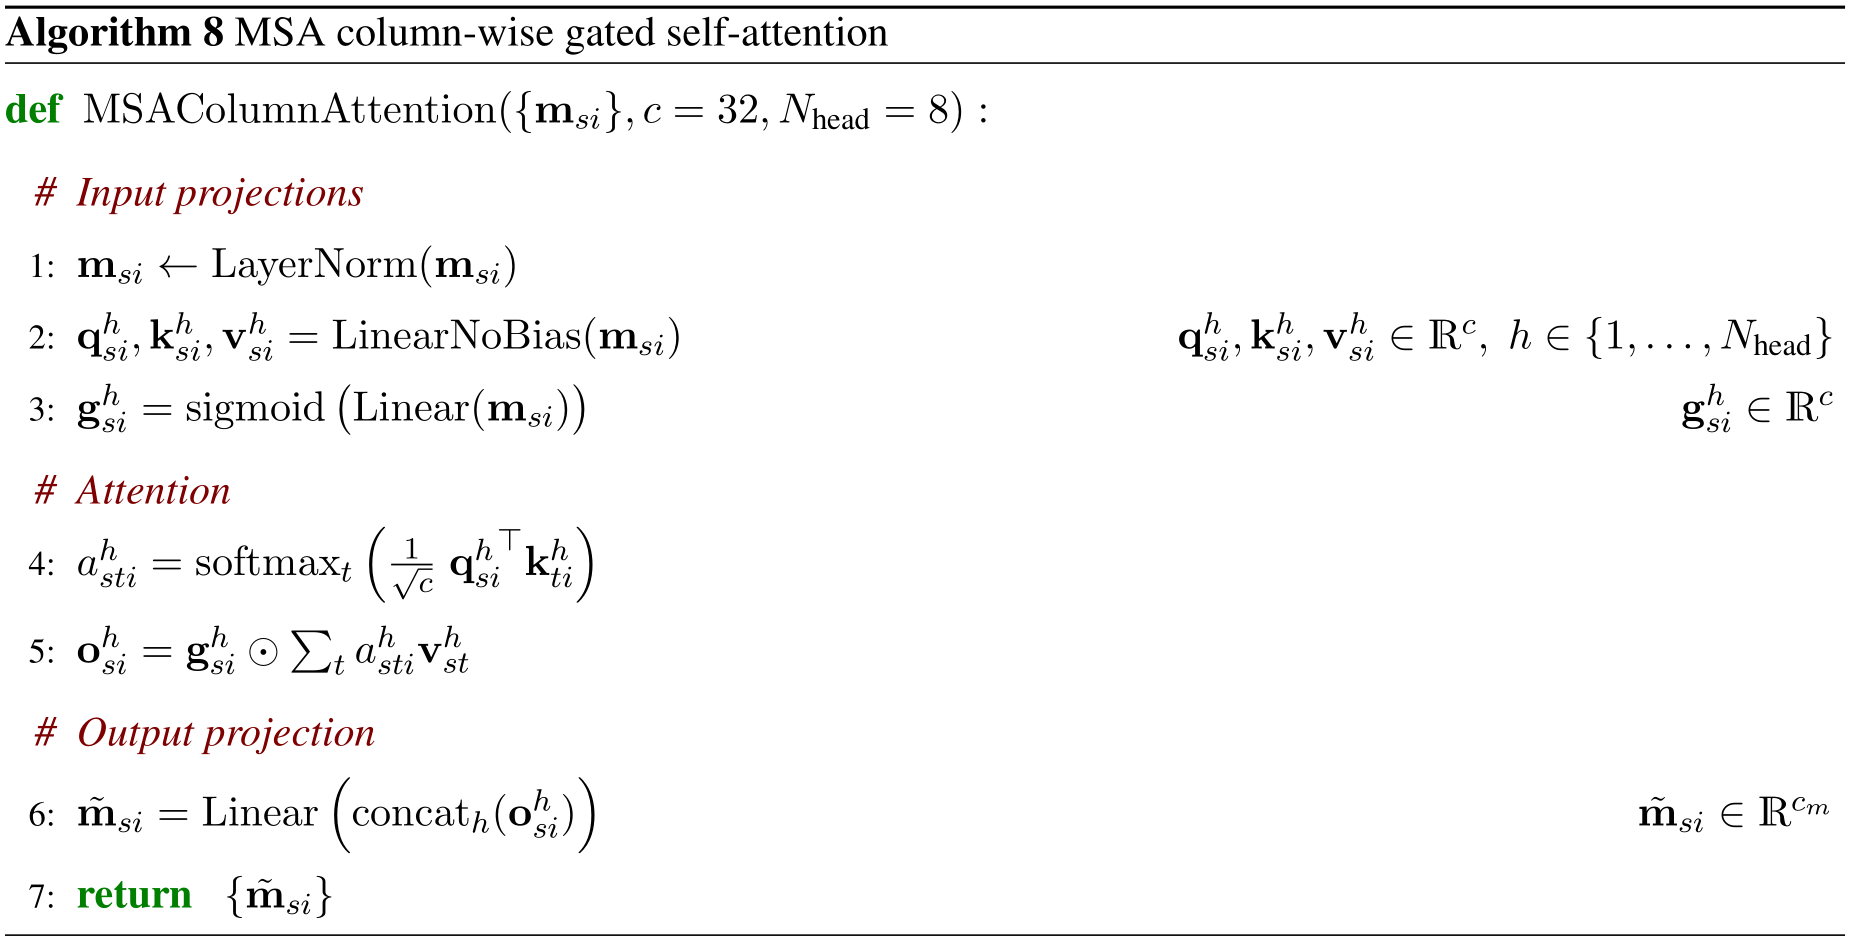
\includegraphics[height=0.8\textheight]{./imgs/algo8_evo_col_attention.png}
\end{center}
\end{frame}

\begin{frame}[label={sec:orge17c8d4}]{EvoFormer: MSA Translation Layer \cite{jumperHighlyAccurateProtein2021}}
\begin{center}
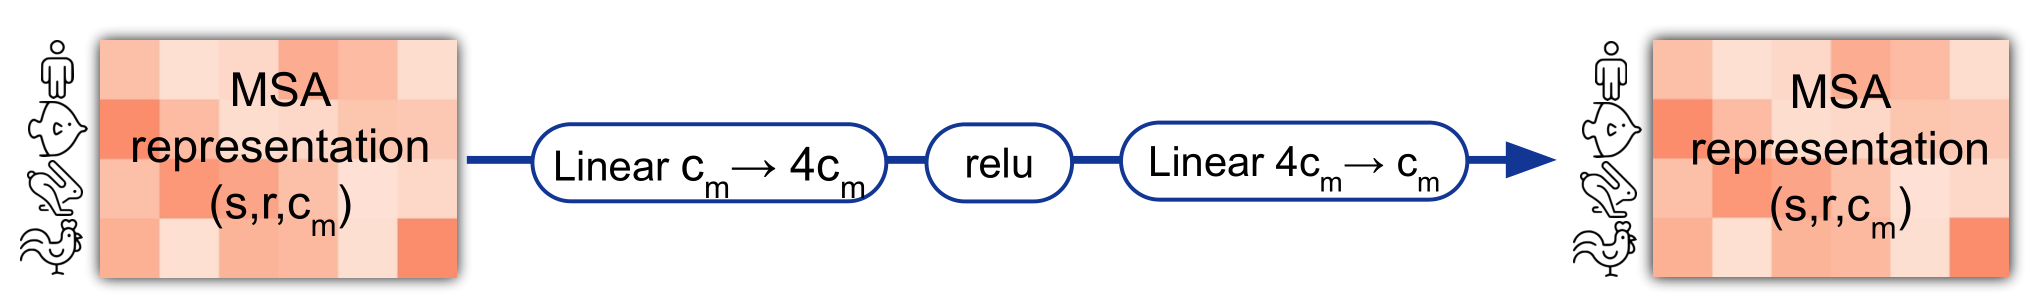
\includegraphics[width=.9\linewidth]{./imgs/msa-translation-layer.png}
\end{center}
\end{frame}

\begin{frame}[label={sec:orga3967f3}]{Algorithm 9 MSA Translation Layer \cite{jumperHighlyAccurateProtein2021}}
\begin{center}
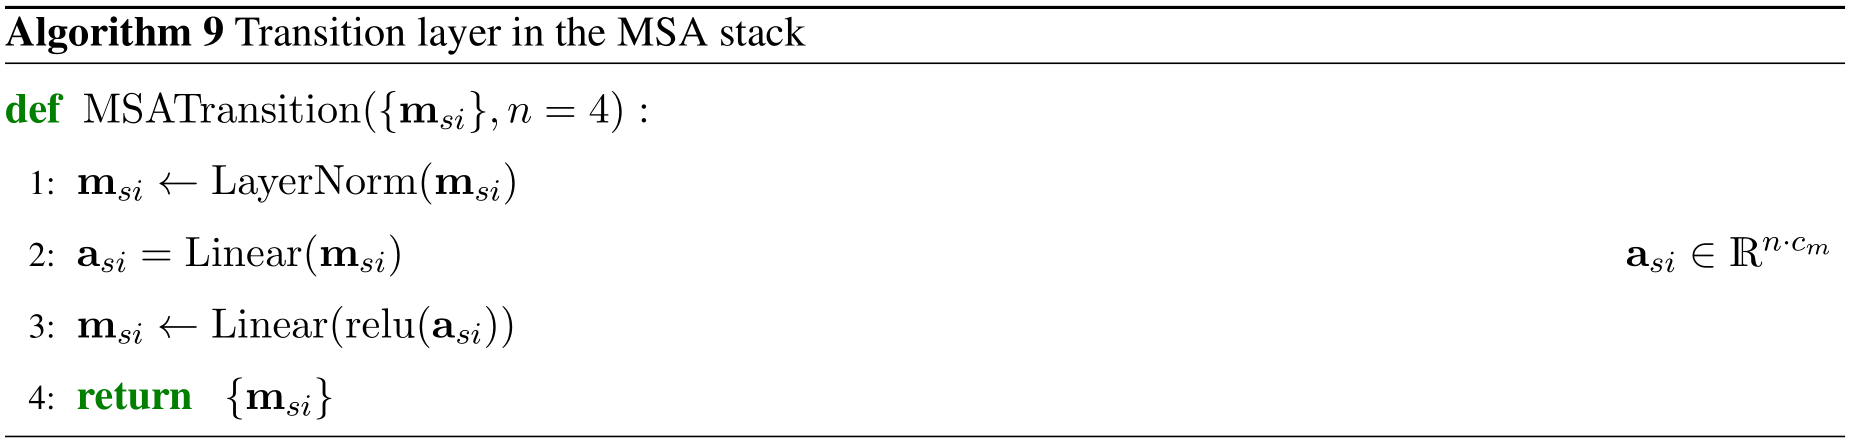
\includegraphics[width=\textwidth]{./imgs/algo9_msa_transition.png}
\end{center}
\end{frame}

\begin{frame}[label={sec:orgc71a7e9}]{EvoFormer: Outer-Product Mean \cite{jumperHighlyAccurateProtein2021}}
\begin{center}
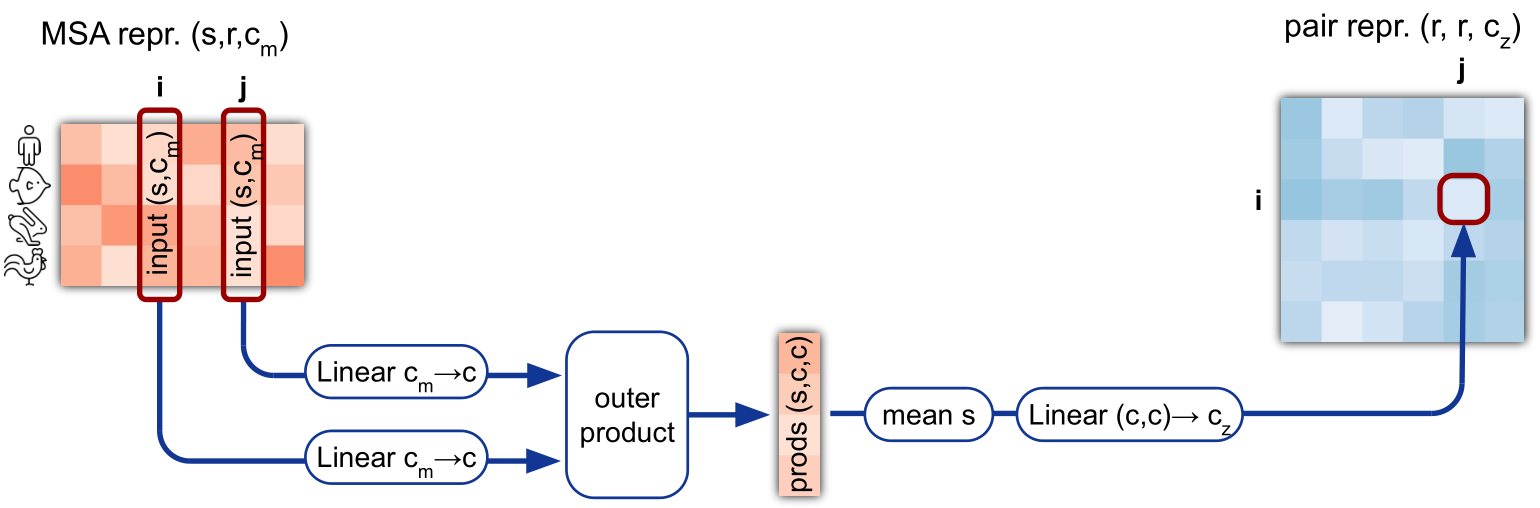
\includegraphics[width=.9\linewidth]{./imgs/outer-product-mean.png}
\end{center}
\end{frame}

\begin{frame}[label={sec:orga4ccaa6}]{Algorithm 10 Outer-Product Mean \cite{jumperHighlyAccurateProtein2021}}
\begin{center}
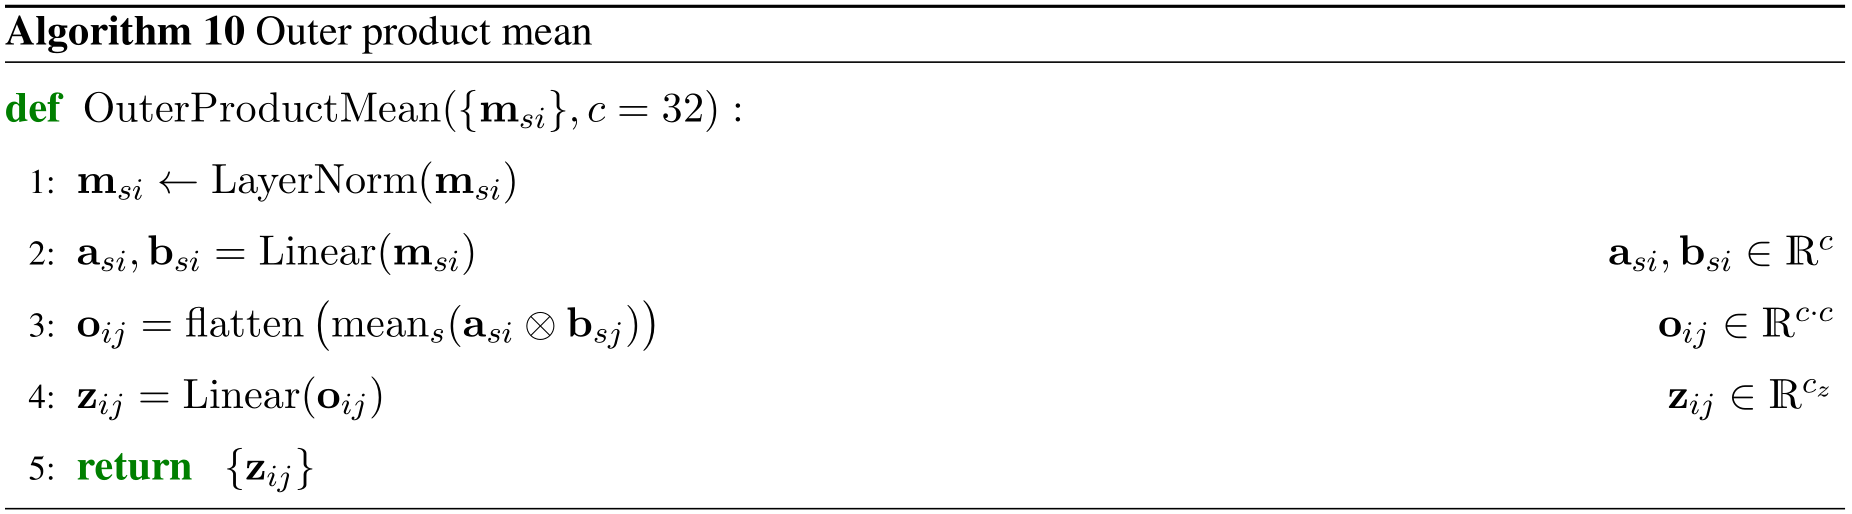
\includegraphics[width=\textwidth]{./imgs/algo10_outer_product.png}
\end{center}
\end{frame}

\begin{frame}[label={sec:org679e68d}]{EvoFormer: Residue Pairs \cite{jumperHighlyAccurateProtein2021}}
\begin{center}
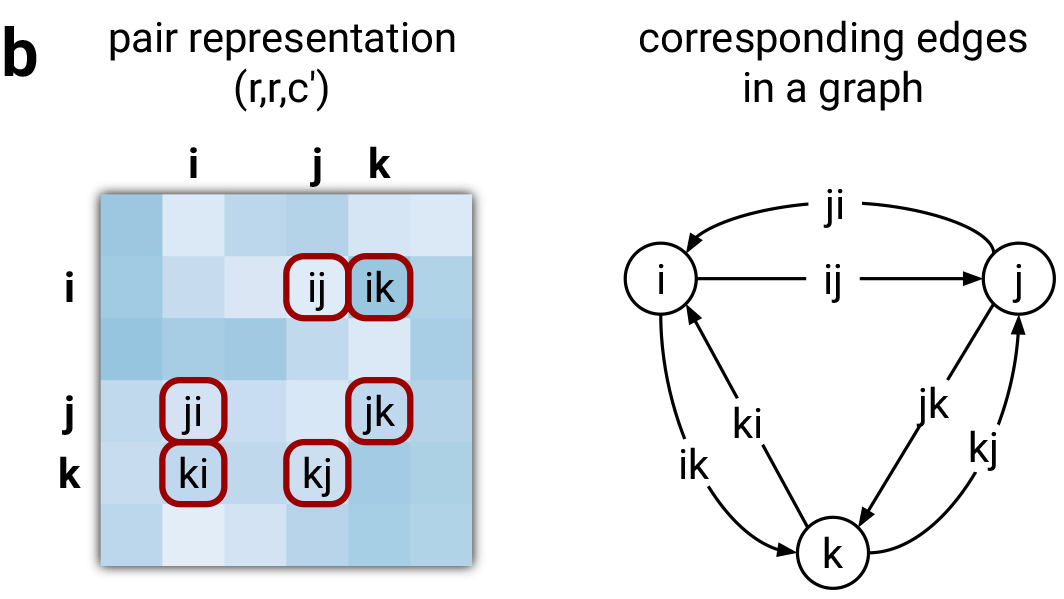
\includegraphics[scale=0.2]{./imgs/model-evoformer-pair1.png}
\end{center}
\begin{center}
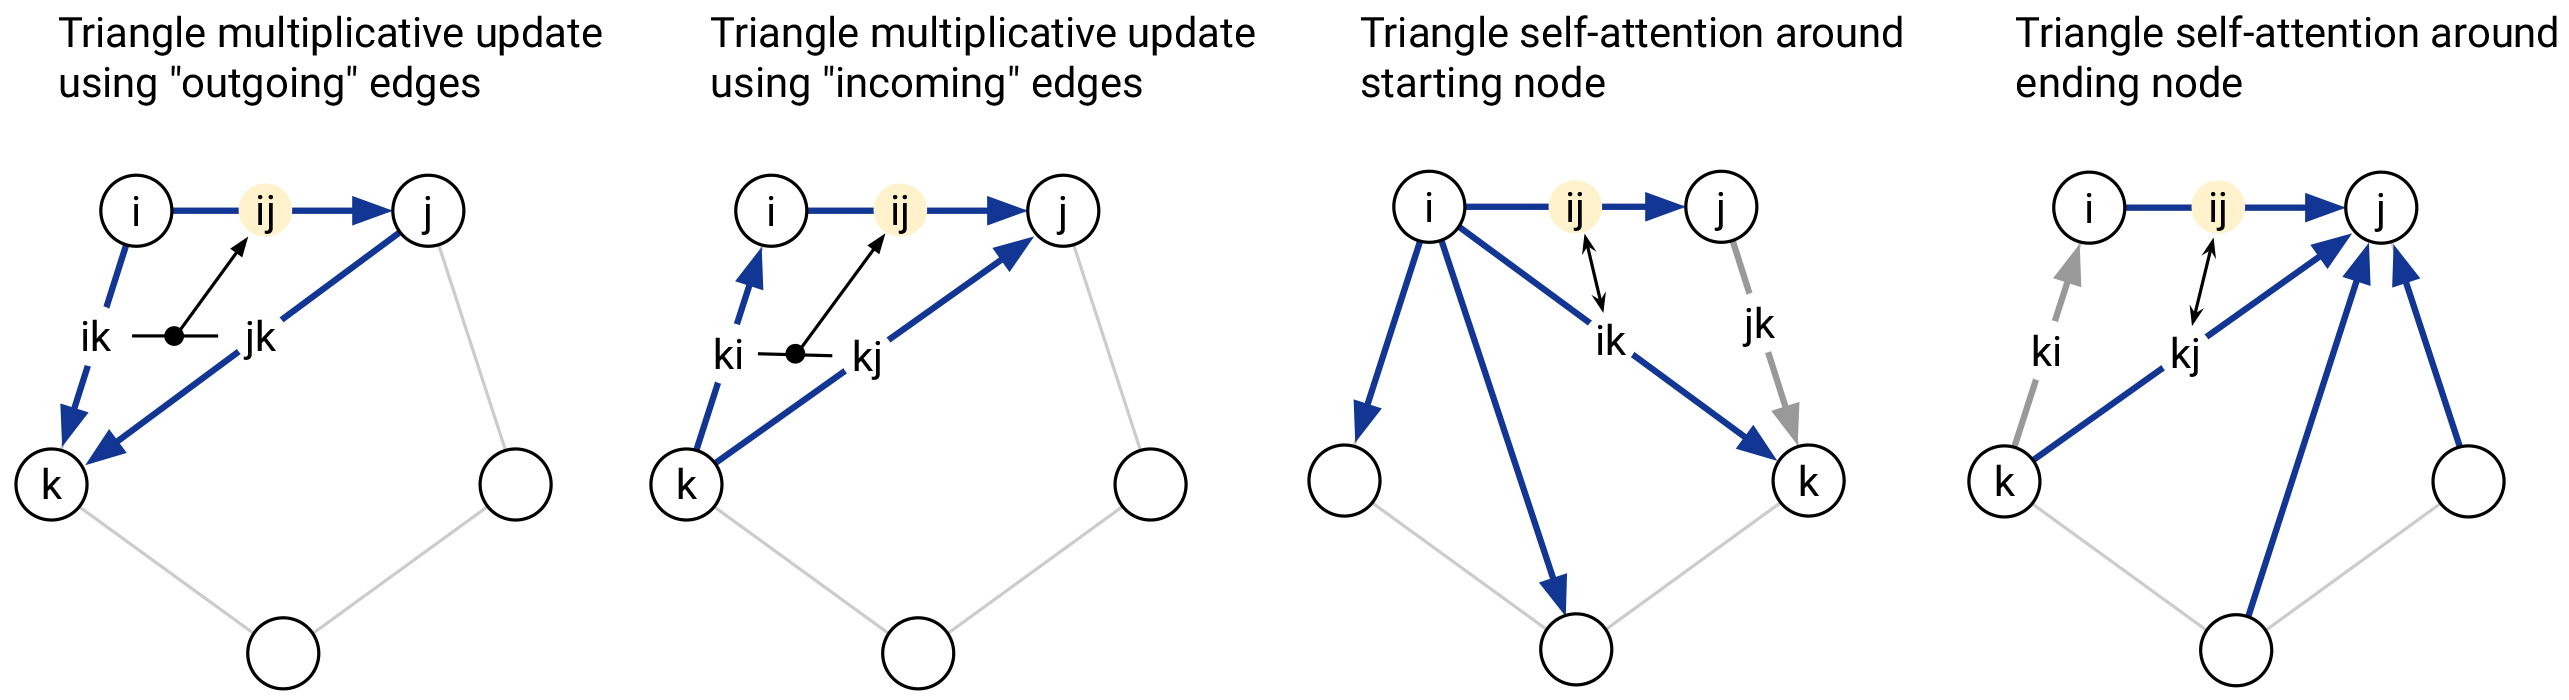
\includegraphics[scale=0.15]{./imgs/model-evoformer-pair2.png}
\end{center}
\end{frame}

\begin{frame}[label={sec:orgaf33686}]{EvoFormer: Triangular Multiplicative Update \cite{jumperHighlyAccurateProtein2021}}
\begin{center}
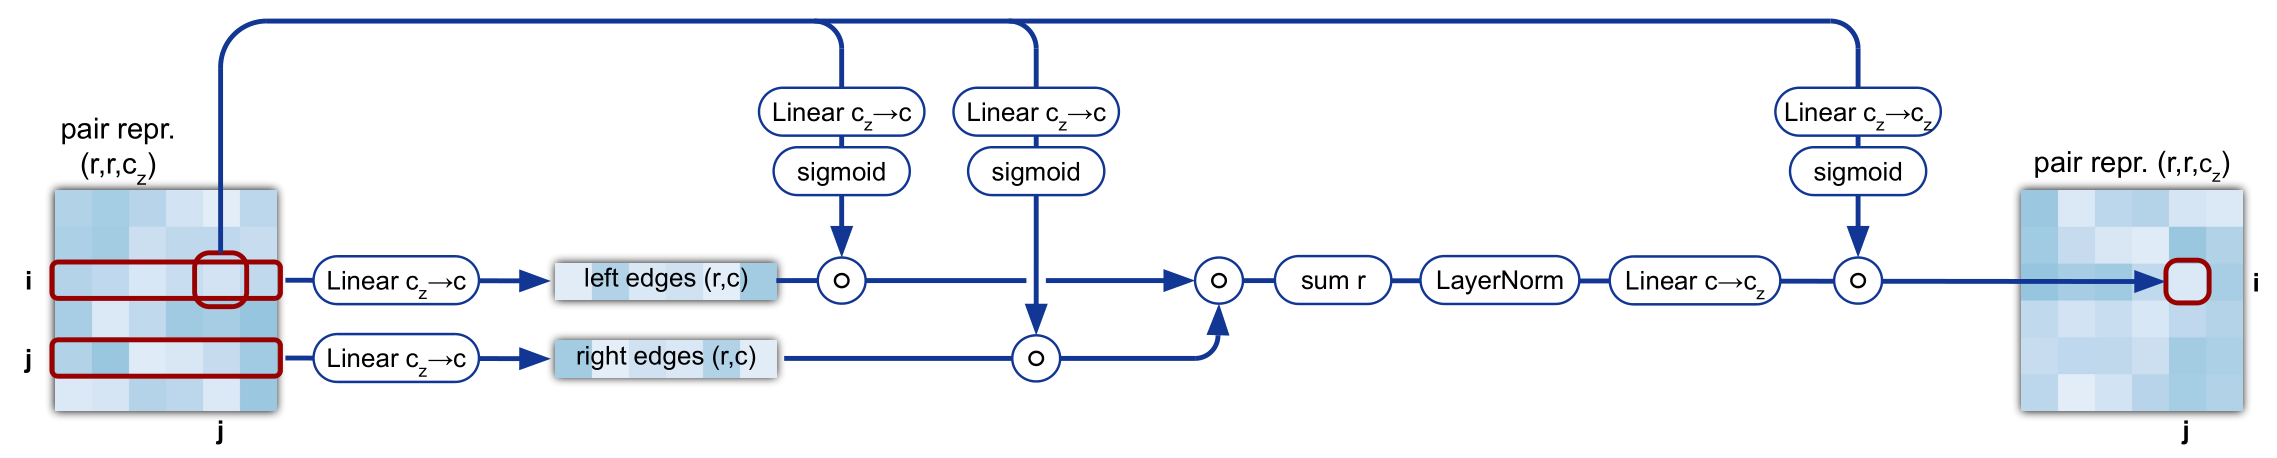
\includegraphics[width=.9\linewidth]{./imgs/triangular-mult-update.png}
\end{center}
\end{frame}

\begin{frame}[label={sec:org99567e2}]{Algorithm 11 Triangular Multiplicative Update: outward \cite{jumperHighlyAccurateProtein2021}}
\begin{center}
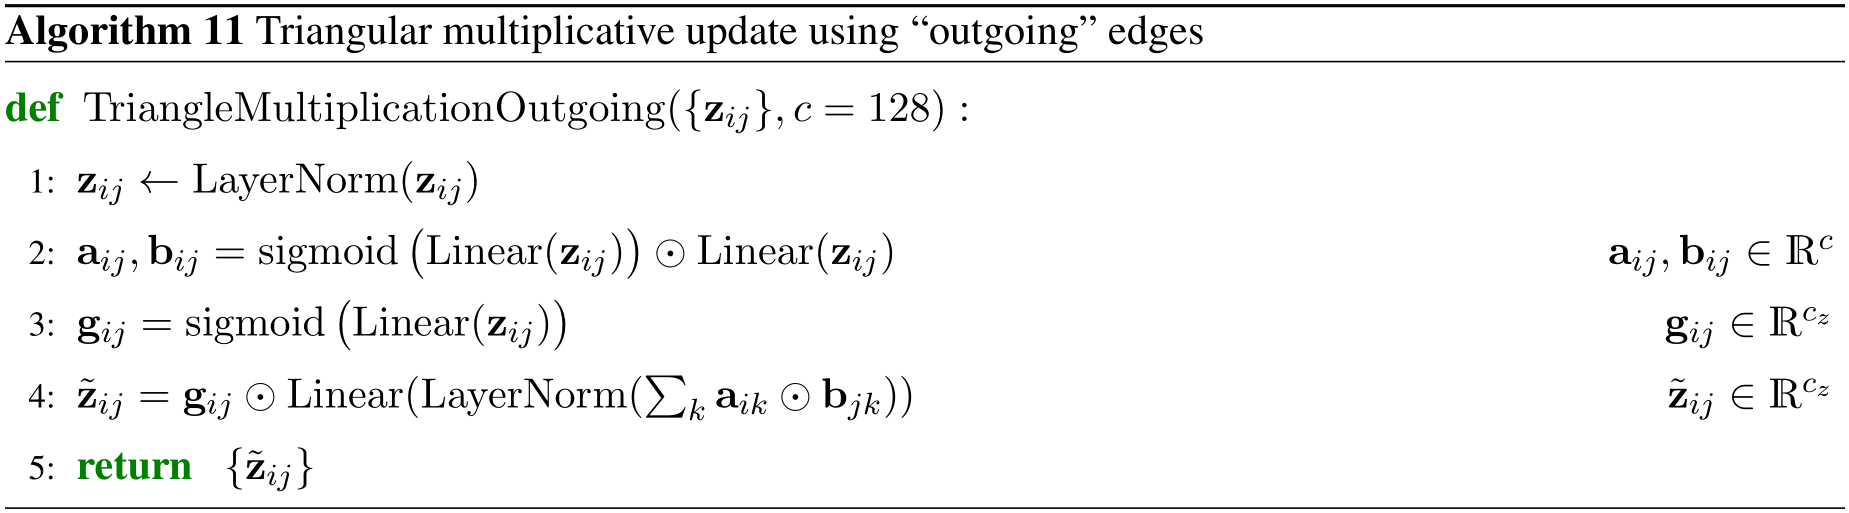
\includegraphics[width=.9\linewidth]{./imgs/algo11_triangular_out.png}
\end{center}
\end{frame}

\begin{frame}[label={sec:org71ff72f}]{Algorithm 12 Triangular Multiplicative Update: inward \cite{jumperHighlyAccurateProtein2021}}
\begin{center}
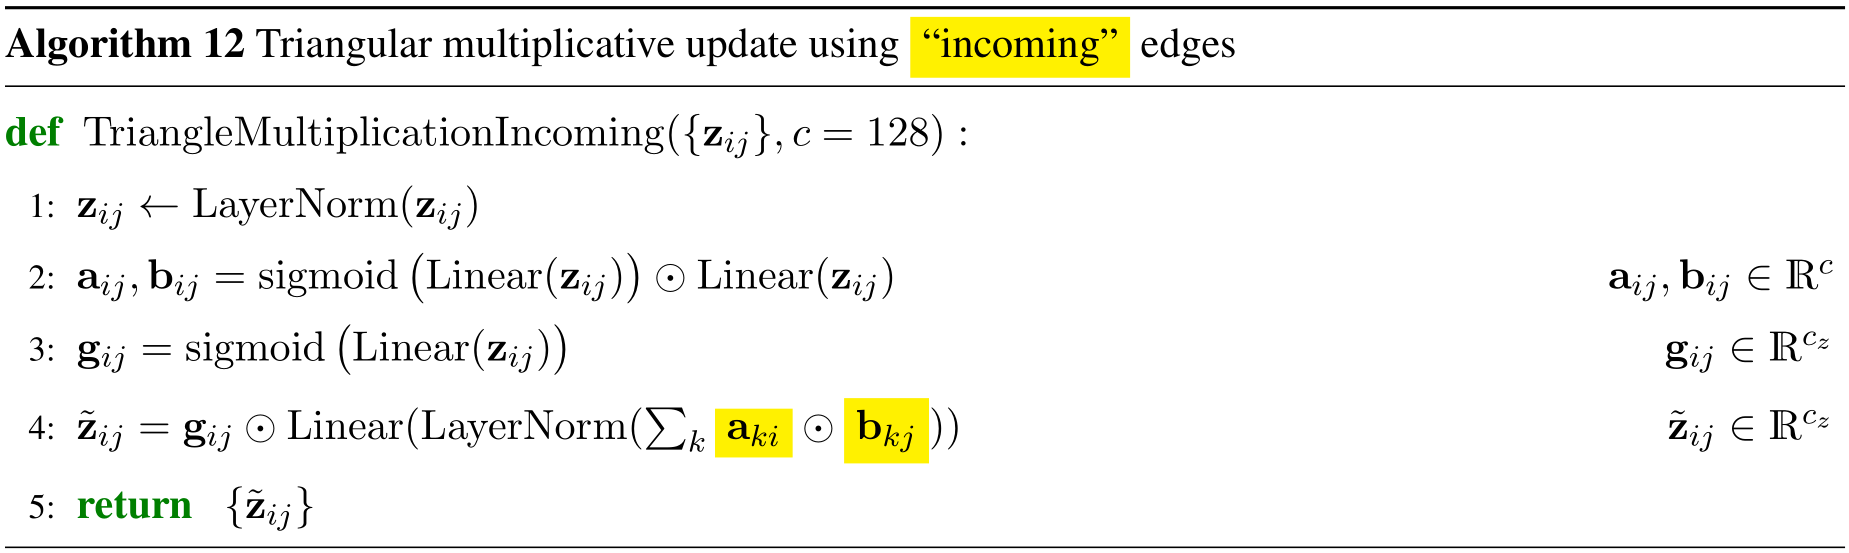
\includegraphics[width=.9\linewidth]{./imgs/algo12_triangular_in.png}
\end{center}
\end{frame}

\begin{frame}[label={sec:org50389f8}]{EvoFormer: Triangular Self-Attention \cite{jumperHighlyAccurateProtein2021}}
\begin{center}
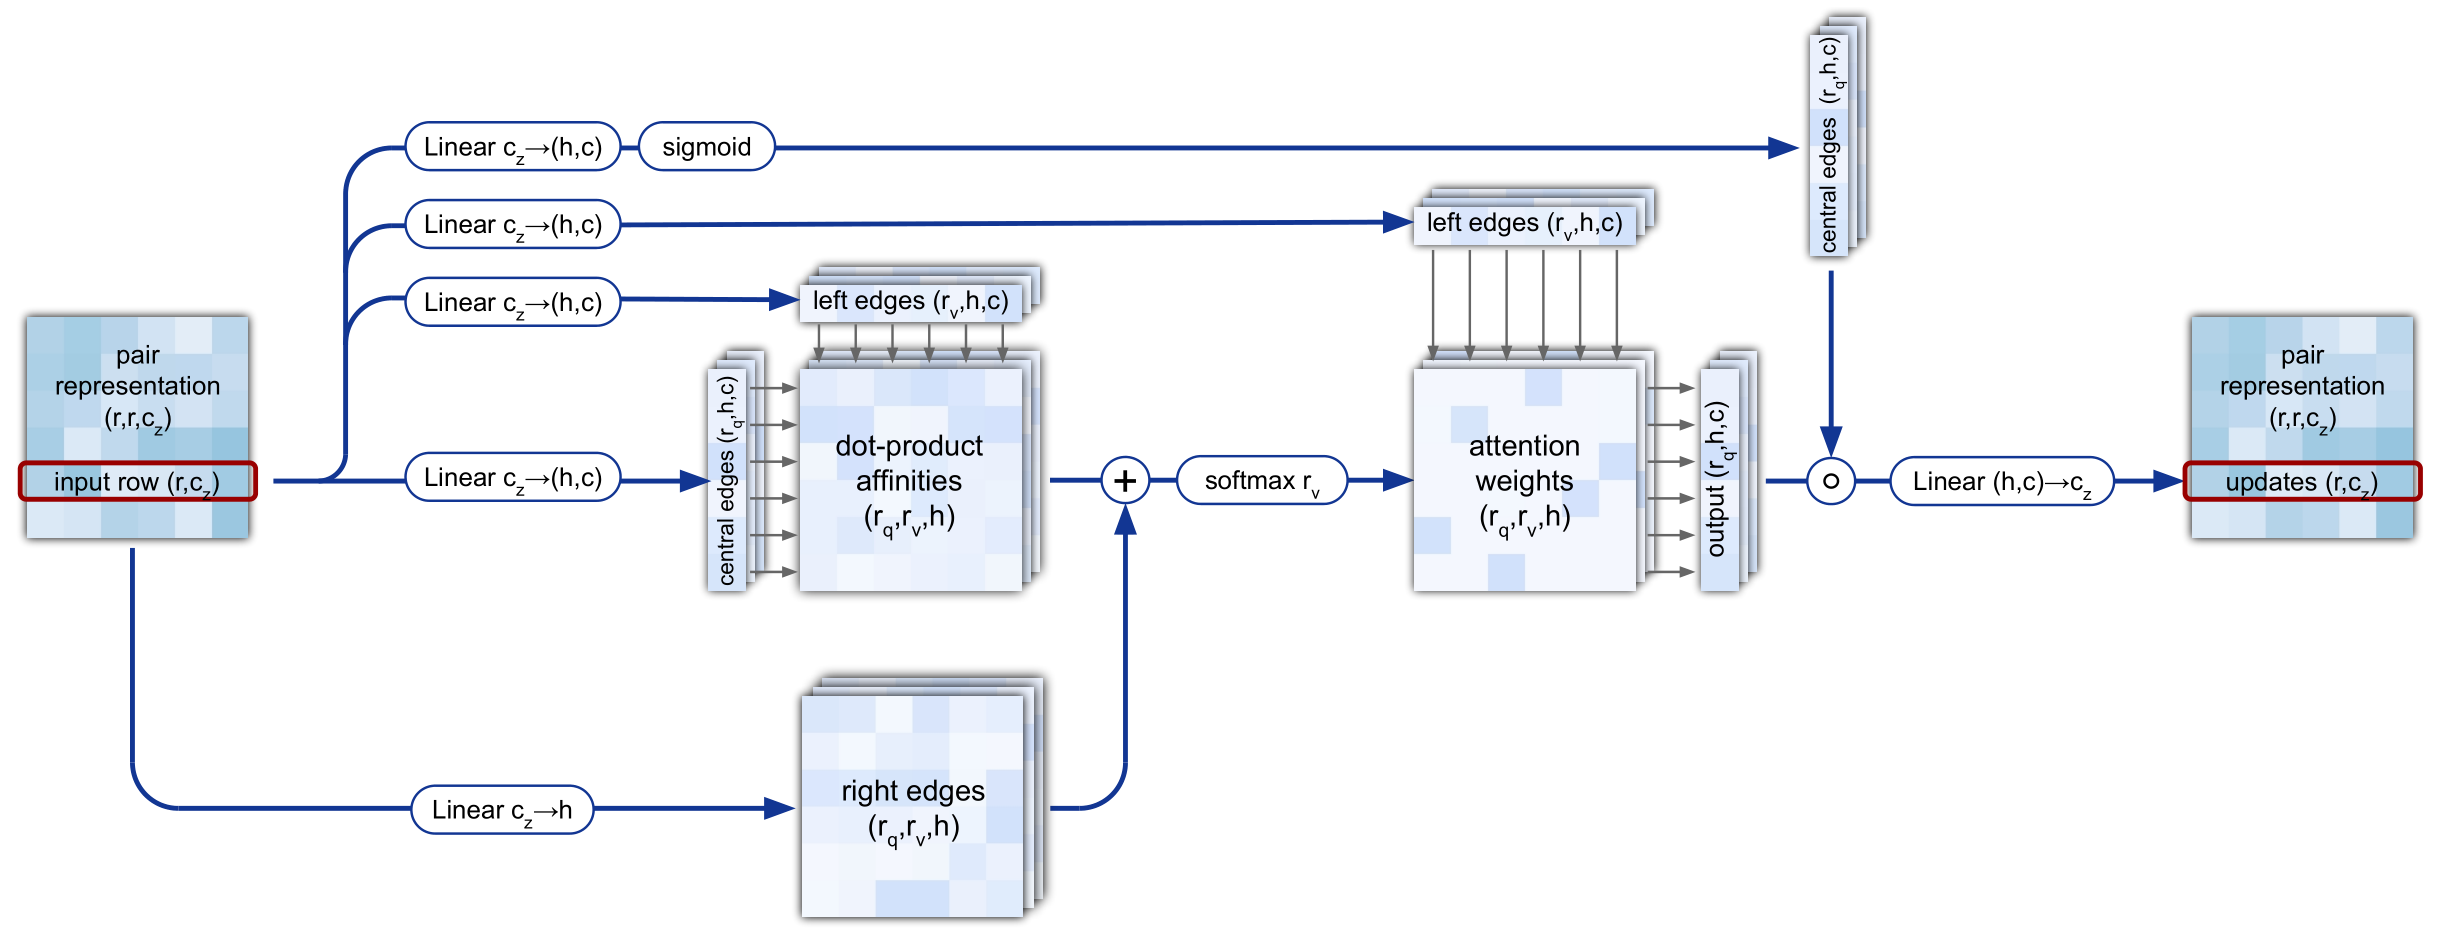
\includegraphics[width=.9\linewidth]{./imgs/triangular-self-attention.png}
\end{center}
\end{frame}
\begin{frame}[label={sec:orgc6da15e}]{Algorithm 13 Triangular Self-Attention: start \cite{jumperHighlyAccurateProtein2021}}
\begin{center}
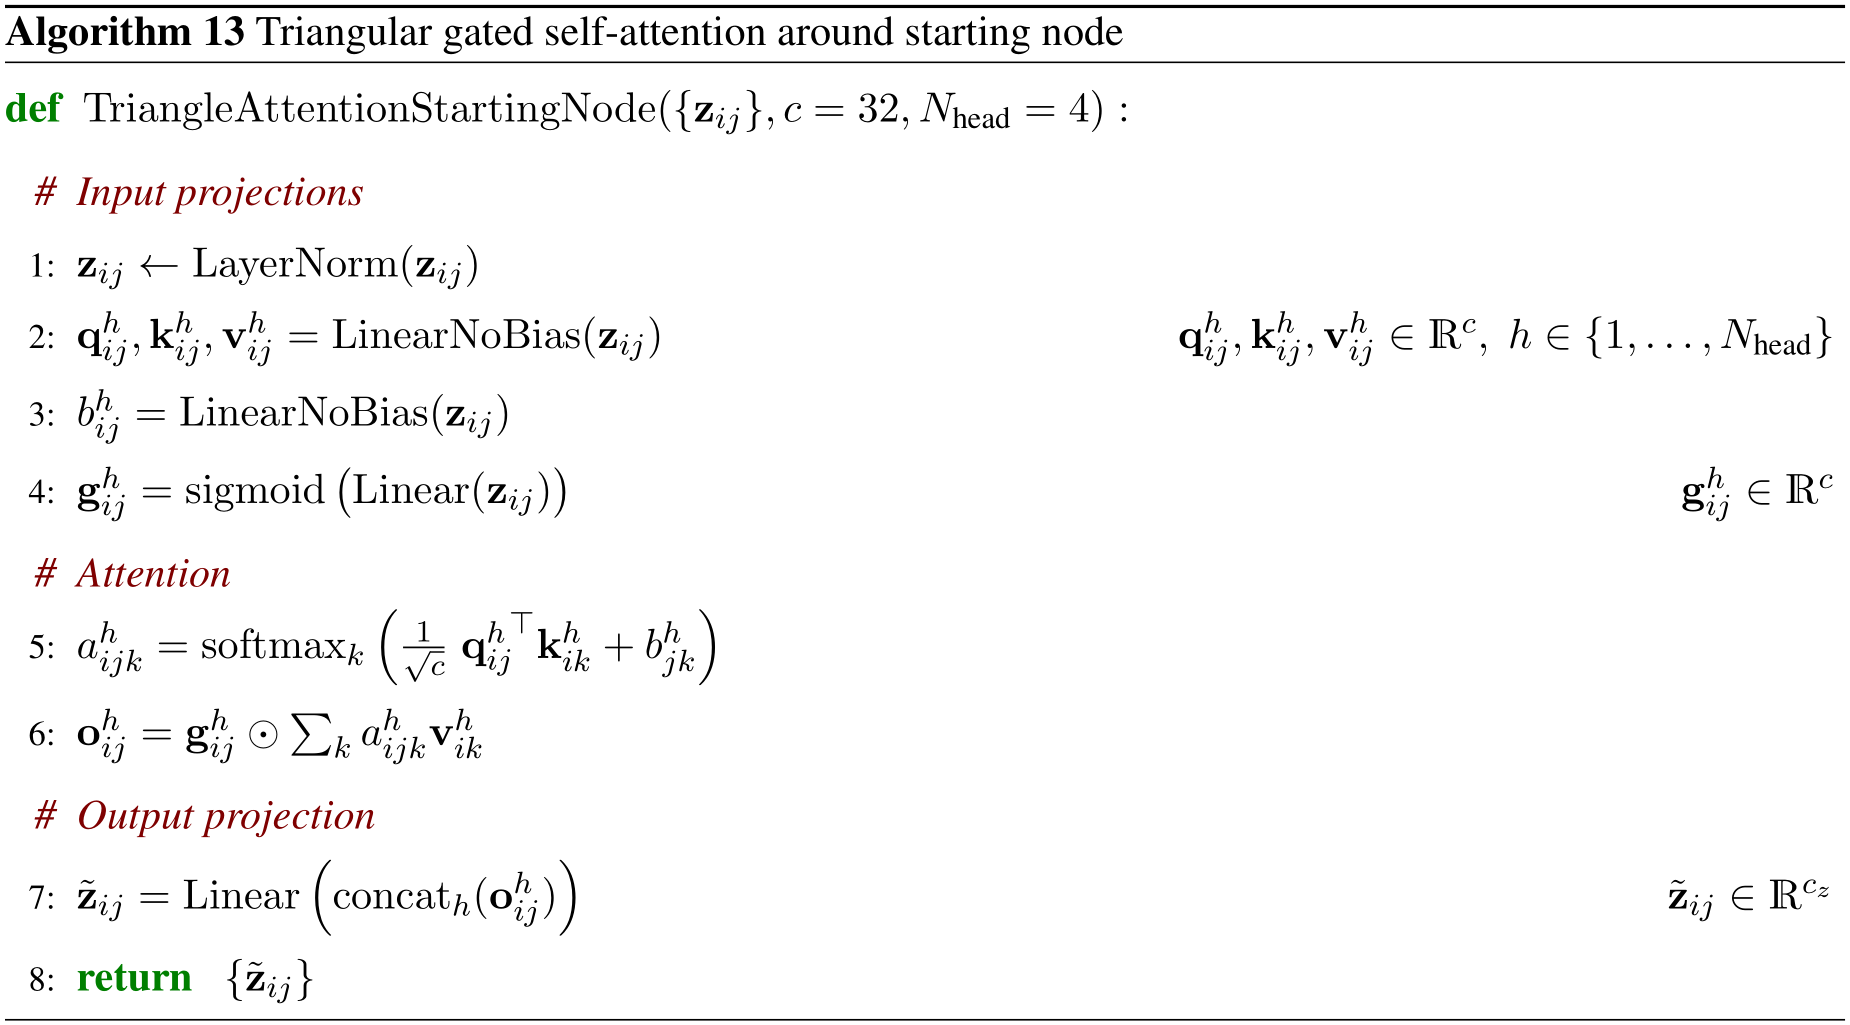
\includegraphics[height=0.9\textheight]{./imgs/algo13_triangular_attention_start.png}
\end{center}
\end{frame}

\begin{frame}[label={sec:orgd75c0ba}]{Algorithm 14 Triangular Self-Attention: end  \cite{jumperHighlyAccurateProtein2021}}
\begin{center}
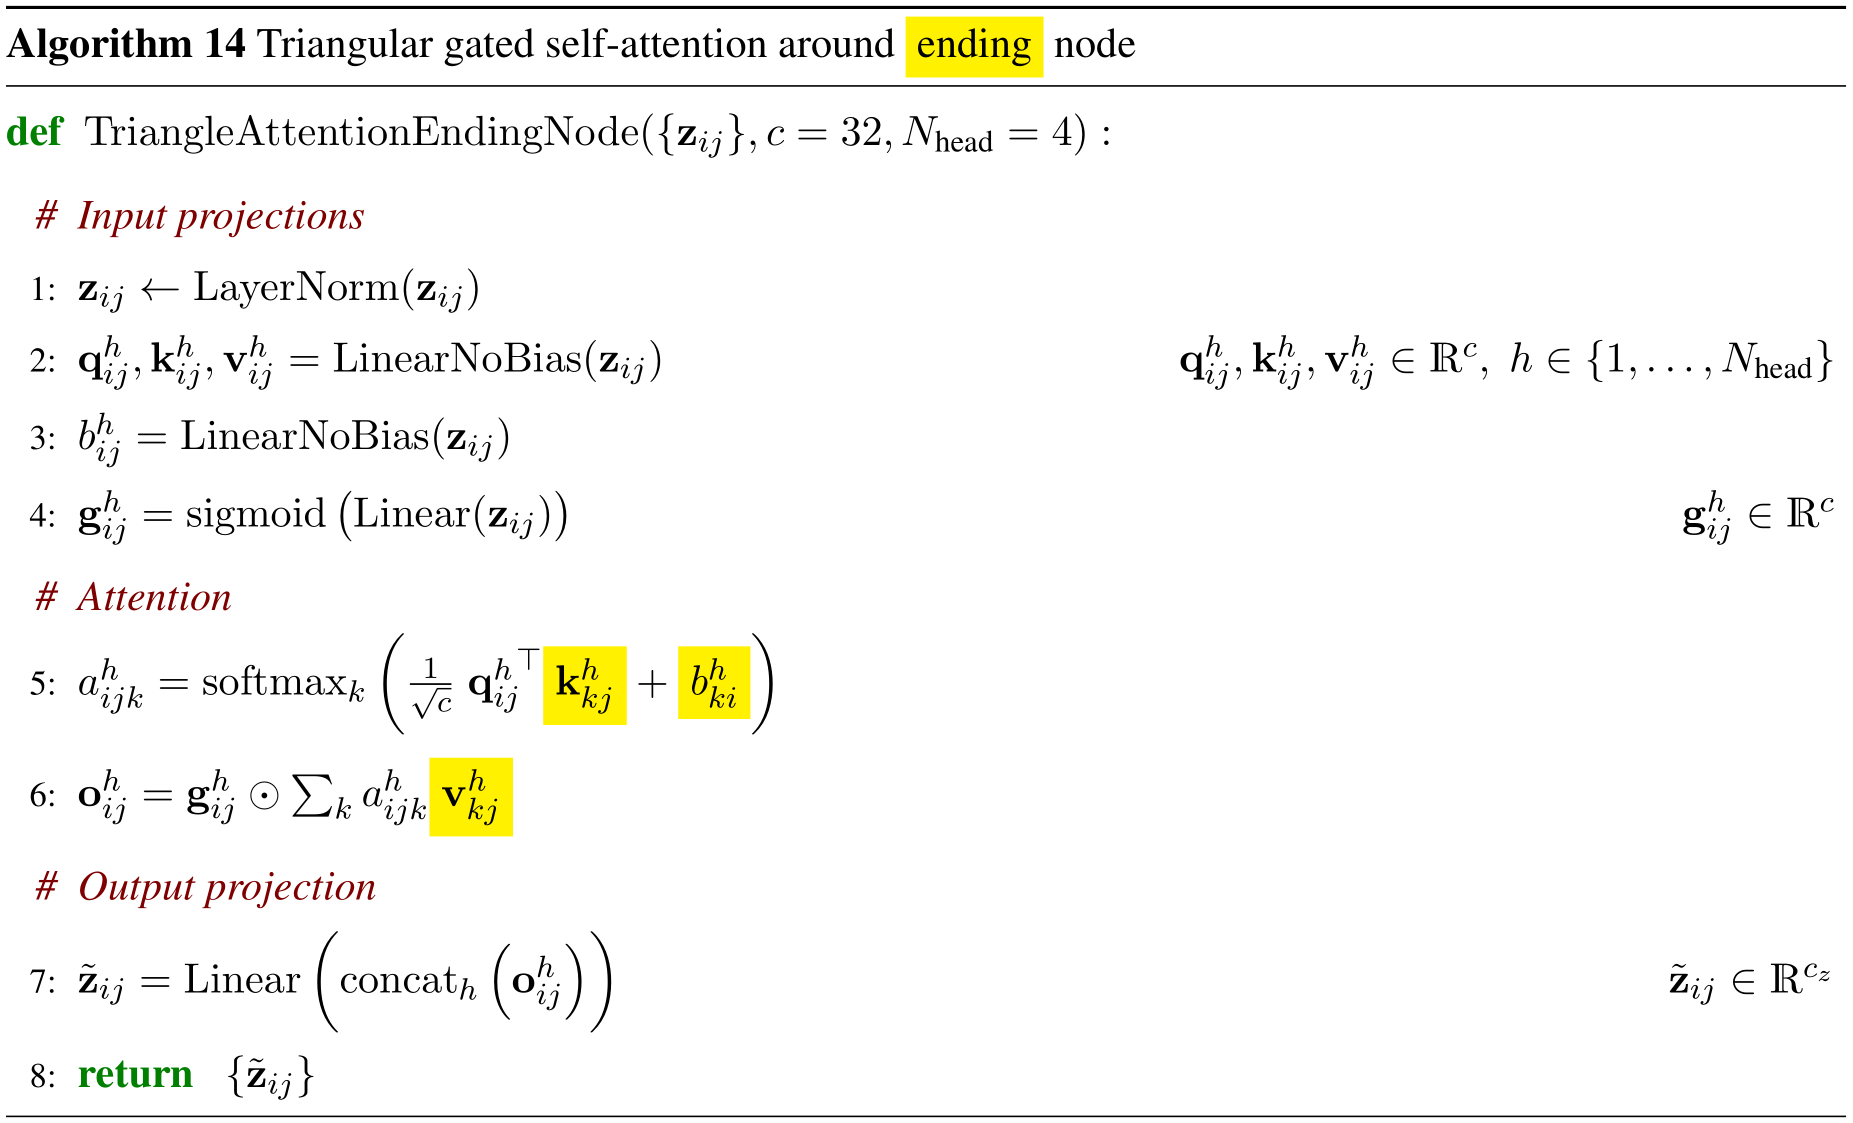
\includegraphics[height=0.9\textheight]{./imgs/algo14_triangular_end.png}
\end{center}
\end{frame}

\begin{frame}[label={sec:org3b8c13b}]{Algorithm 15 Transition layer in the pair stack \cite{jumperHighlyAccurateProtein2021}}
\begin{center}
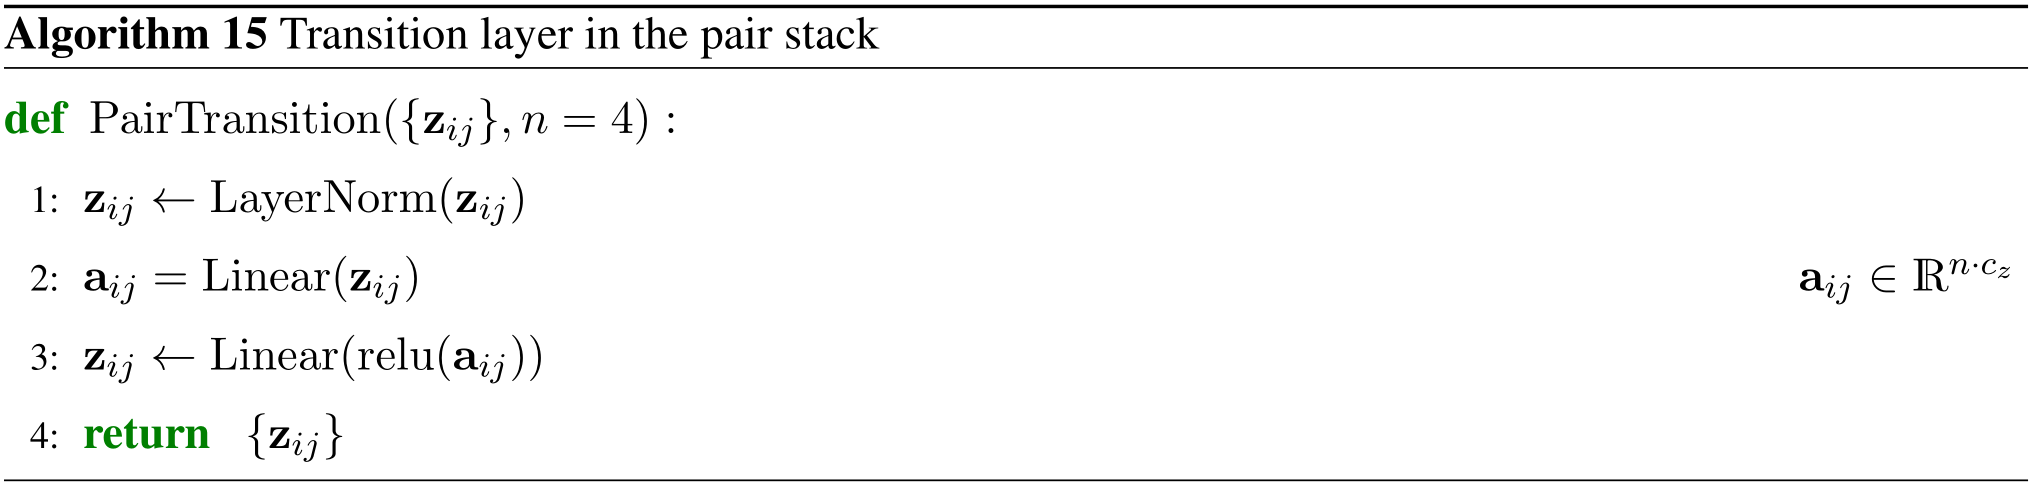
\includegraphics[width=.9\linewidth]{./imgs/algo15_pair_transition.png}
\end{center}
\end{frame}

\begin{frame}[label={sec:org6a9f006}]{Algorithm 16 Template pair stack \cite{jumperHighlyAccurateProtein2021}}
\begin{center}
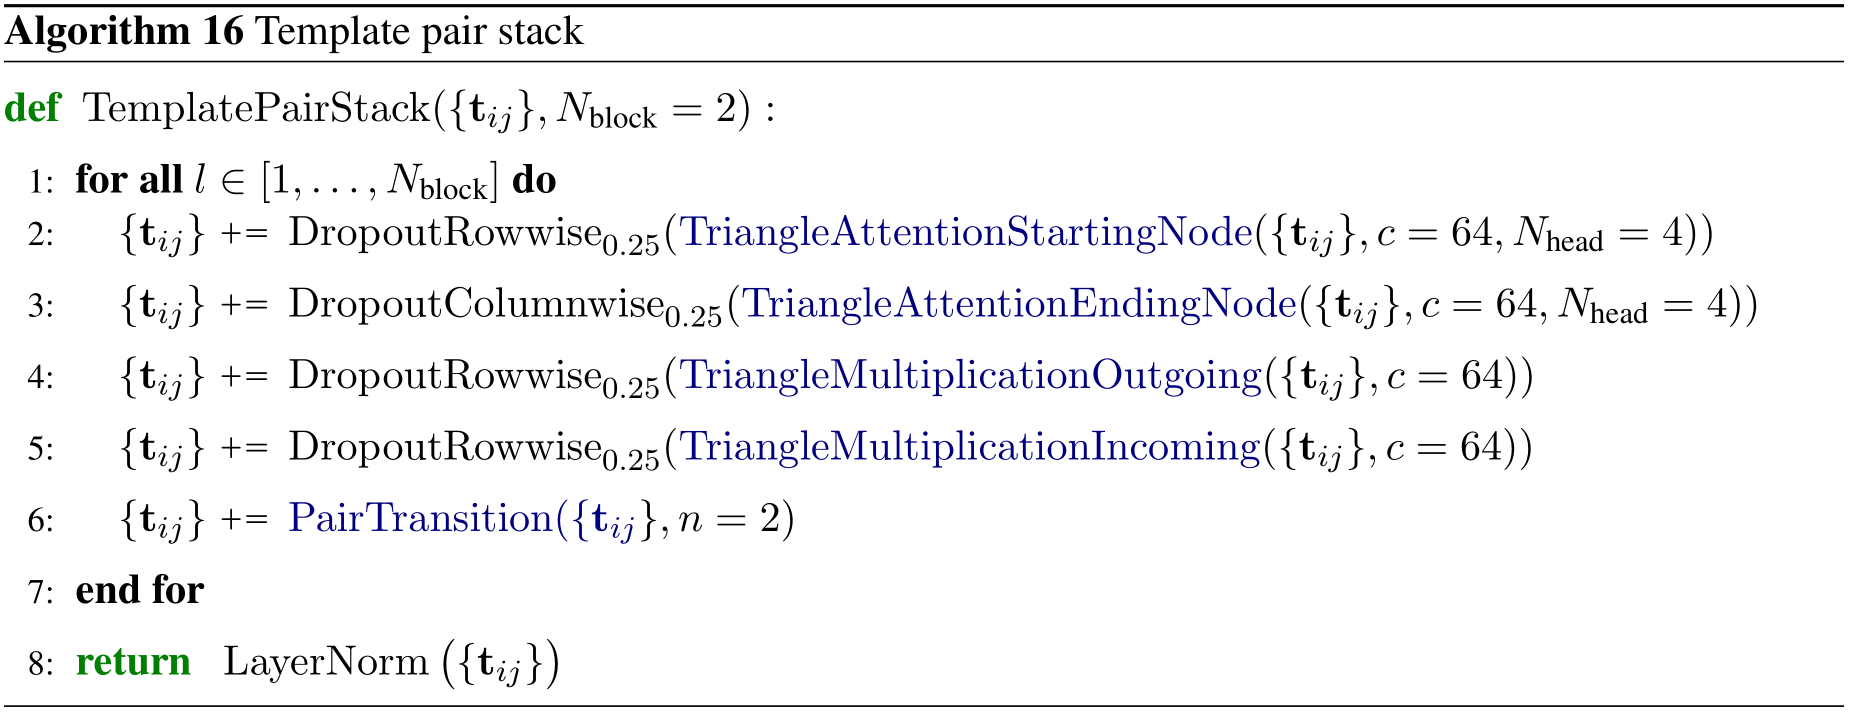
\includegraphics[width=.9\linewidth]{./imgs/algo16_template_pair_stack.png}
\end{center}
\end{frame}
\begin{frame}[label={sec:org151b2fc}]{Algorithm 17 Template pointwise attention \cite{jumperHighlyAccurateProtein2021}}
\begin{center}
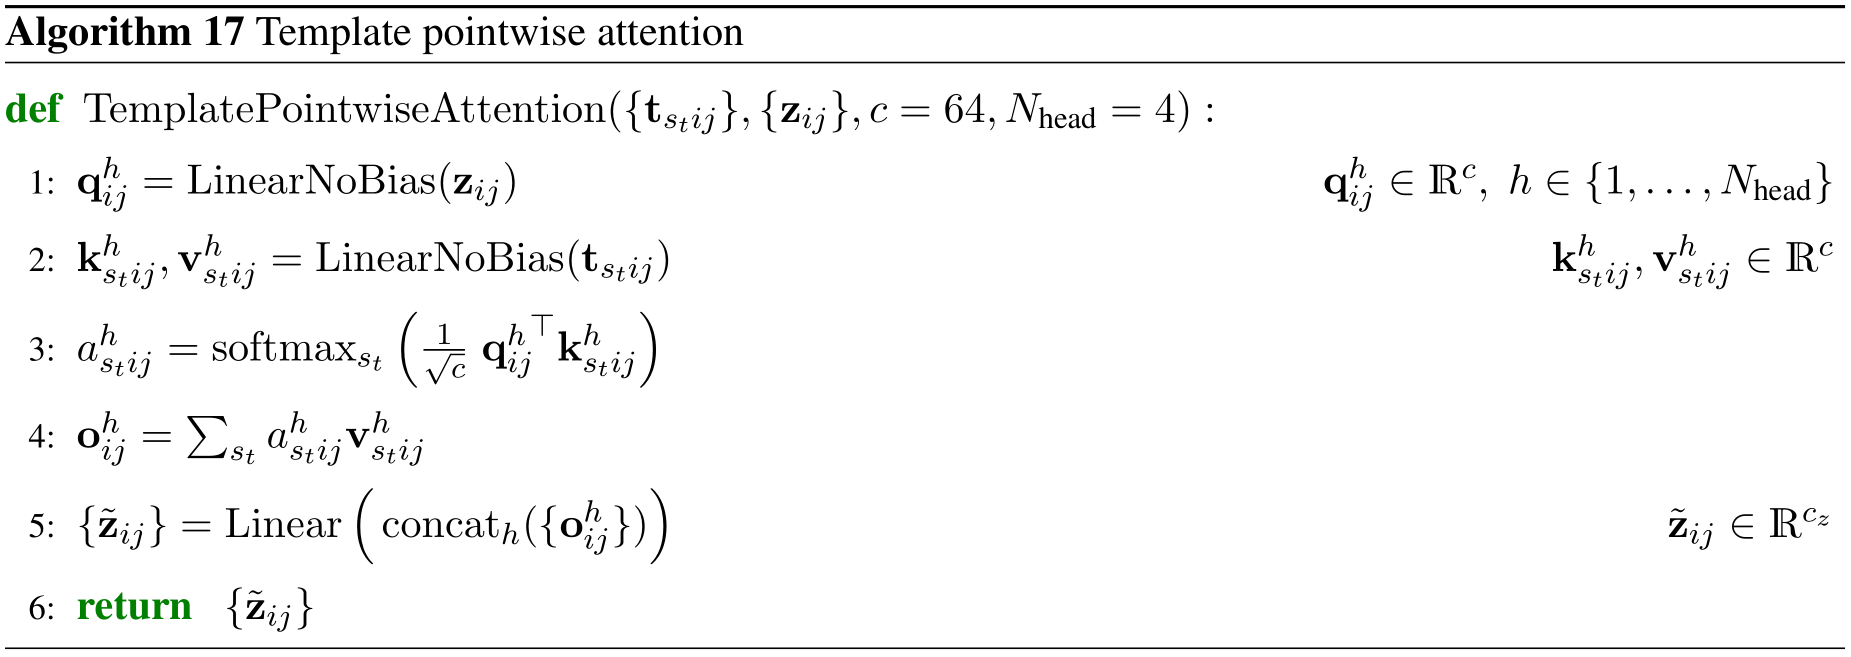
\includegraphics[width=\textwidth]{./imgs/algo17_template_point_attention.png}
\end{center}
\end{frame}

\begin{frame}[label={sec:org9d4cc2b}]{Algorithm 18 Extra MSA stack \cite{jumperHighlyAccurateProtein2021}}
\begin{center}
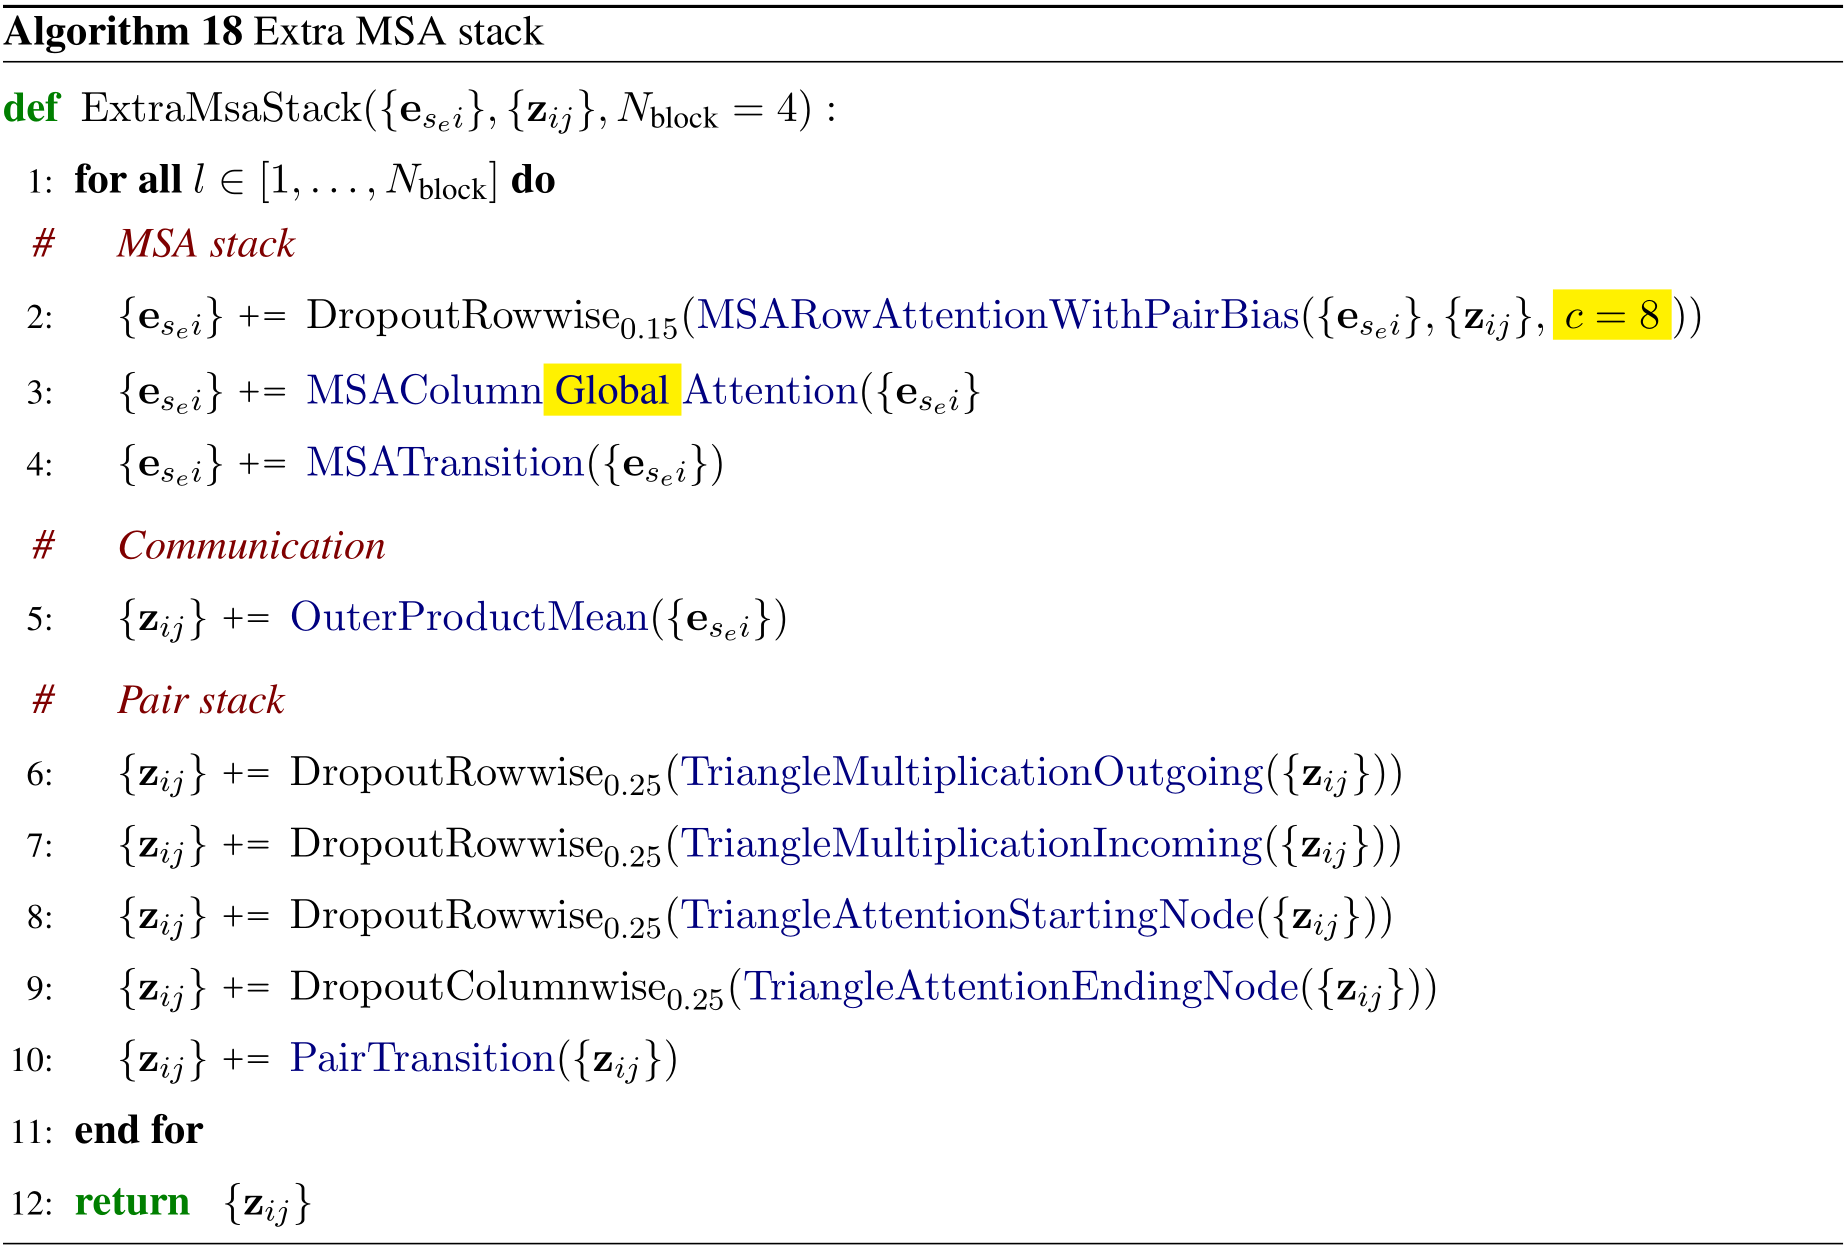
\includegraphics[height=0.9\textheight]{./imgs/algo18_extra_msa_stack.png}
\end{center}
\end{frame}

\begin{frame}[label={sec:org906dc78}]{Algorithm 19 MSA global column-wise gated self-attention \cite{jumperHighlyAccurateProtein2021}}
\begin{center}
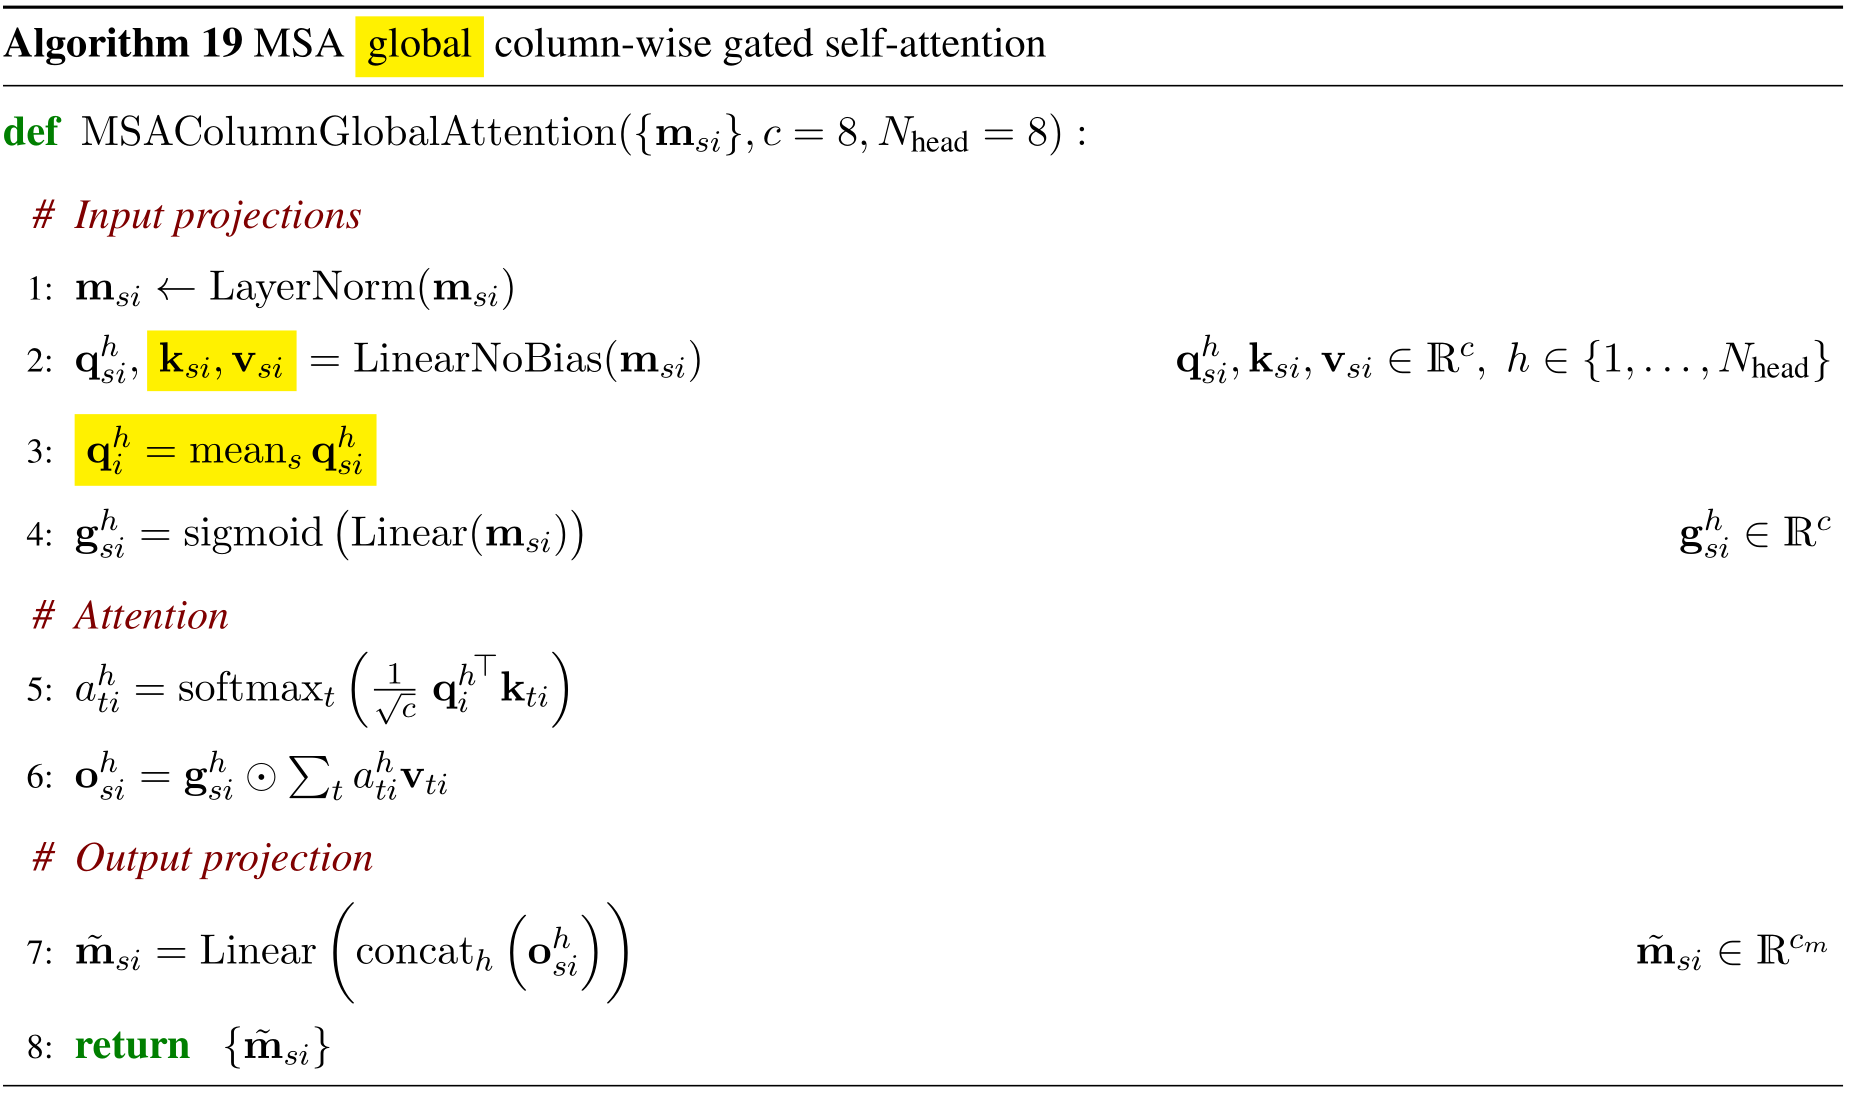
\includegraphics[height=0.9\textheight]{./imgs/algo19_msa_global_col_attention.png}
\end{center}
\end{frame}

\subsection*{Structure Module}
\label{sec:org5470bd9}
\begin{frame}[label={sec:org95d3f6f}]{Structure Module: Overview \cite{jumperHighlyAccurateProtein2021}}
\begin{center}
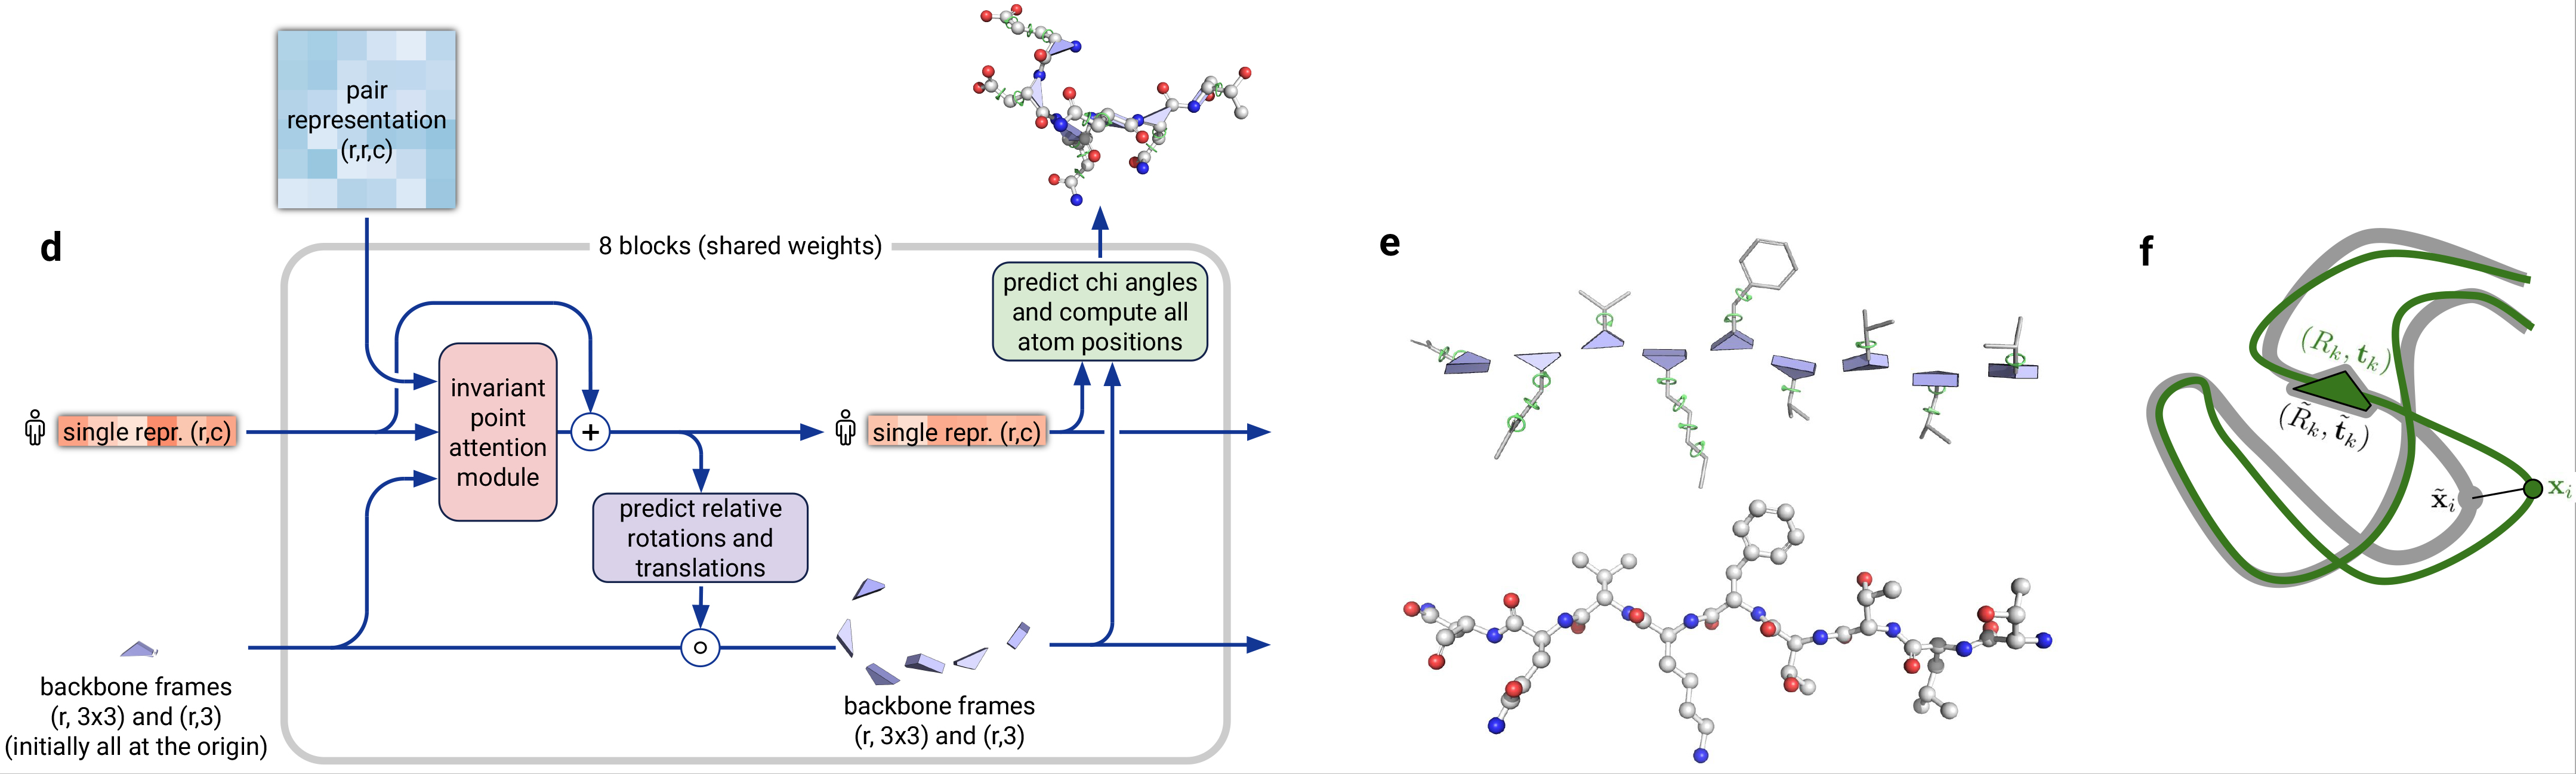
\includegraphics[width=.9\linewidth]{./imgs/model-structure.png}
\end{center}
\end{frame}

\begin{frame}[label={sec:orgbb3629a}]{Structure Module: Frame Representation}
\begin{figure}[htbp]
\centering
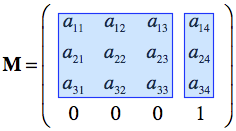
\includegraphics[scale=0.8]{./imgs/TransformationMatrix1.png}
\caption{Example transform \protect\cite{SpatialTransformationMatrices}}
\end{figure}

\begin{itemize}
\item rotation + translation transforms \(T_i := (R_i,t_i)\)
\item no reflection, scaling, or shear
\item they construct ground truth frames using the position of three atoms from the ground truth PDB structures using a Gram–Schmidt process (Algorithm 21)
\end{itemize}
\end{frame}
\begin{frame}[label={sec:org28b432d}]{Structure Module: Invariant point attention (IPA) \cite{jumperHighlyAccurateProtein2021}}
\begin{center}
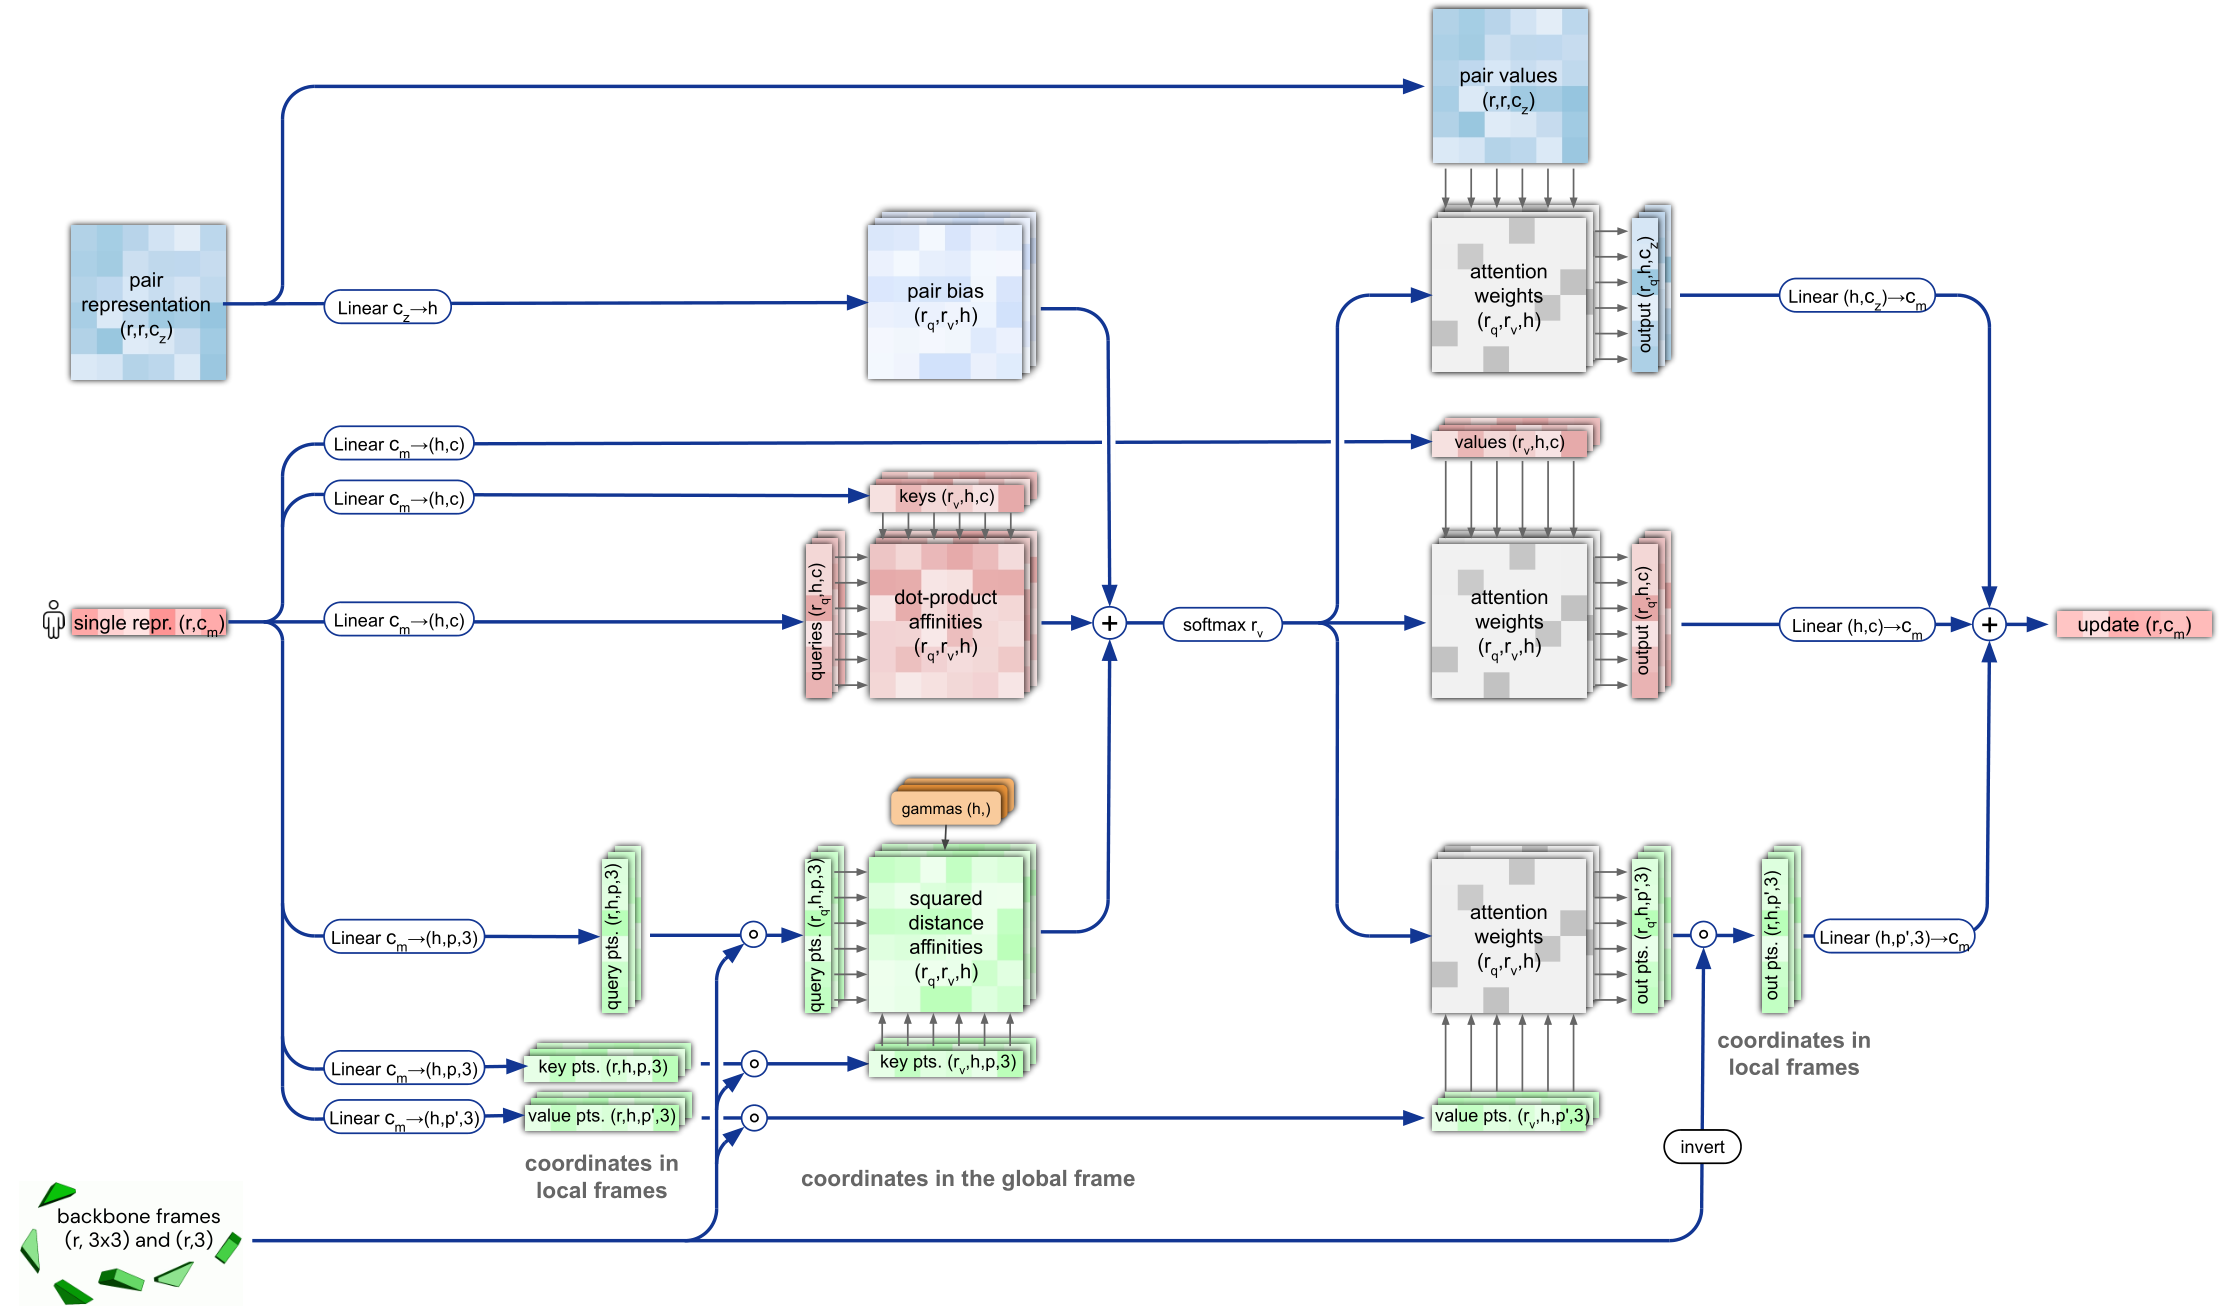
\includegraphics[width=.9\linewidth]{./imgs/ipa.png}
\end{center}
\end{frame}

\begin{frame}[label={sec:orgdd356fb}]{Structure Module: Algorithm Part 1 \cite{jumperHighlyAccurateProtein2021}}
\begin{center}
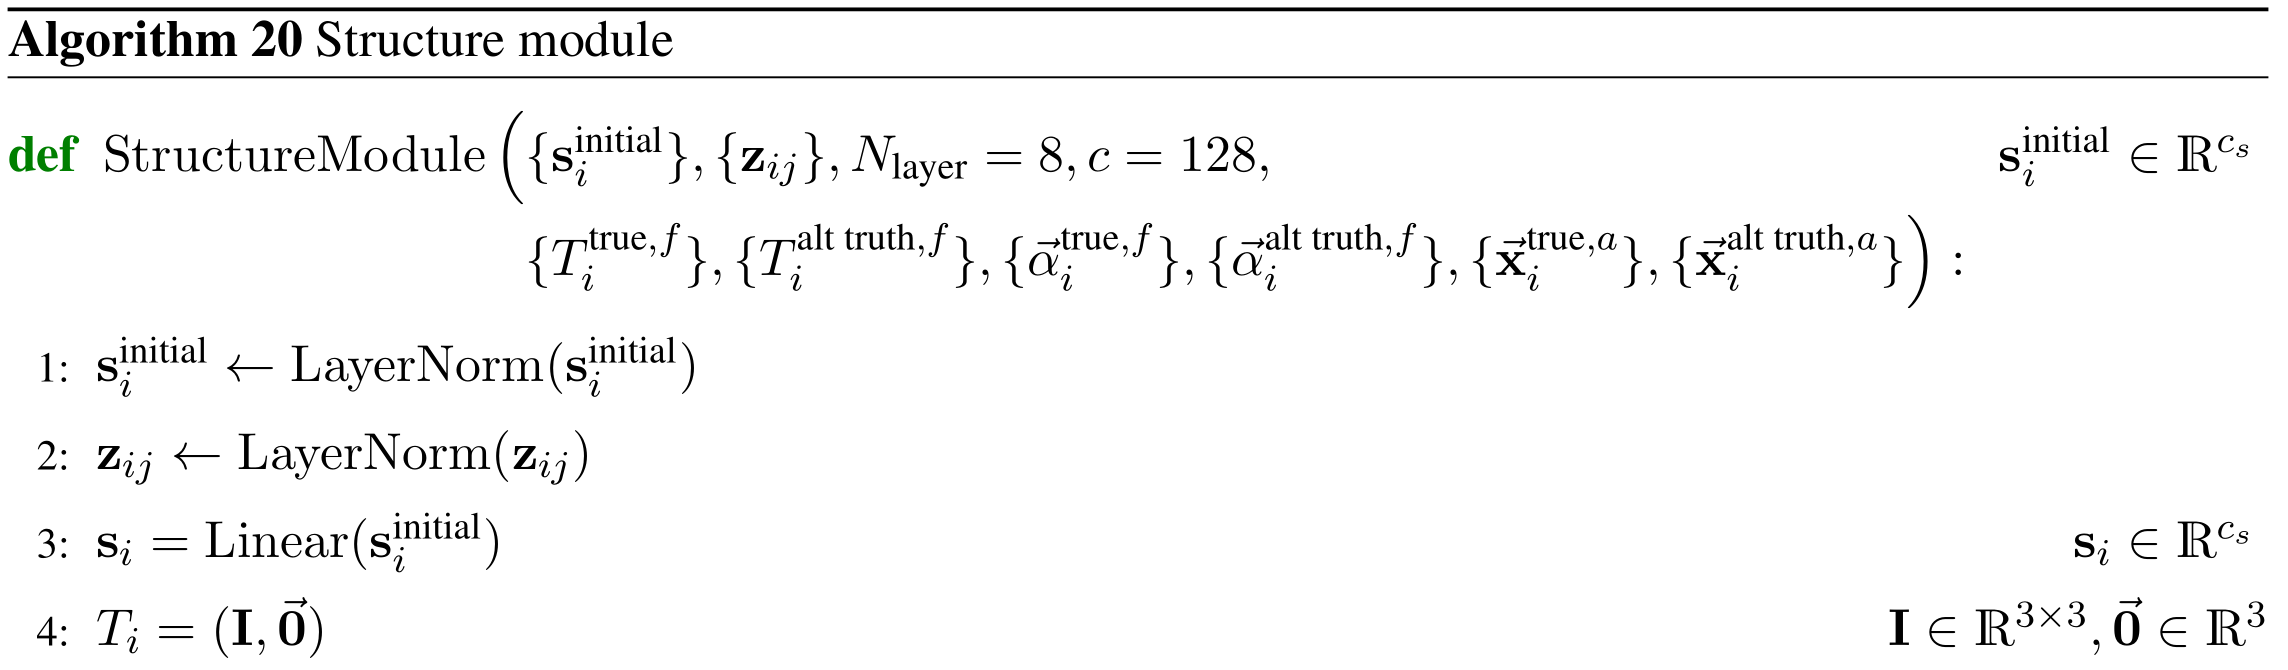
\includegraphics[width=.9\linewidth]{./imgs/algo20-part1.png}
\end{center}
\end{frame}

\begin{frame}[label={sec:orga3e3515}]{Structure Module: Algorithm Part 2 \cite{jumperHighlyAccurateProtein2021}}
\begin{center}
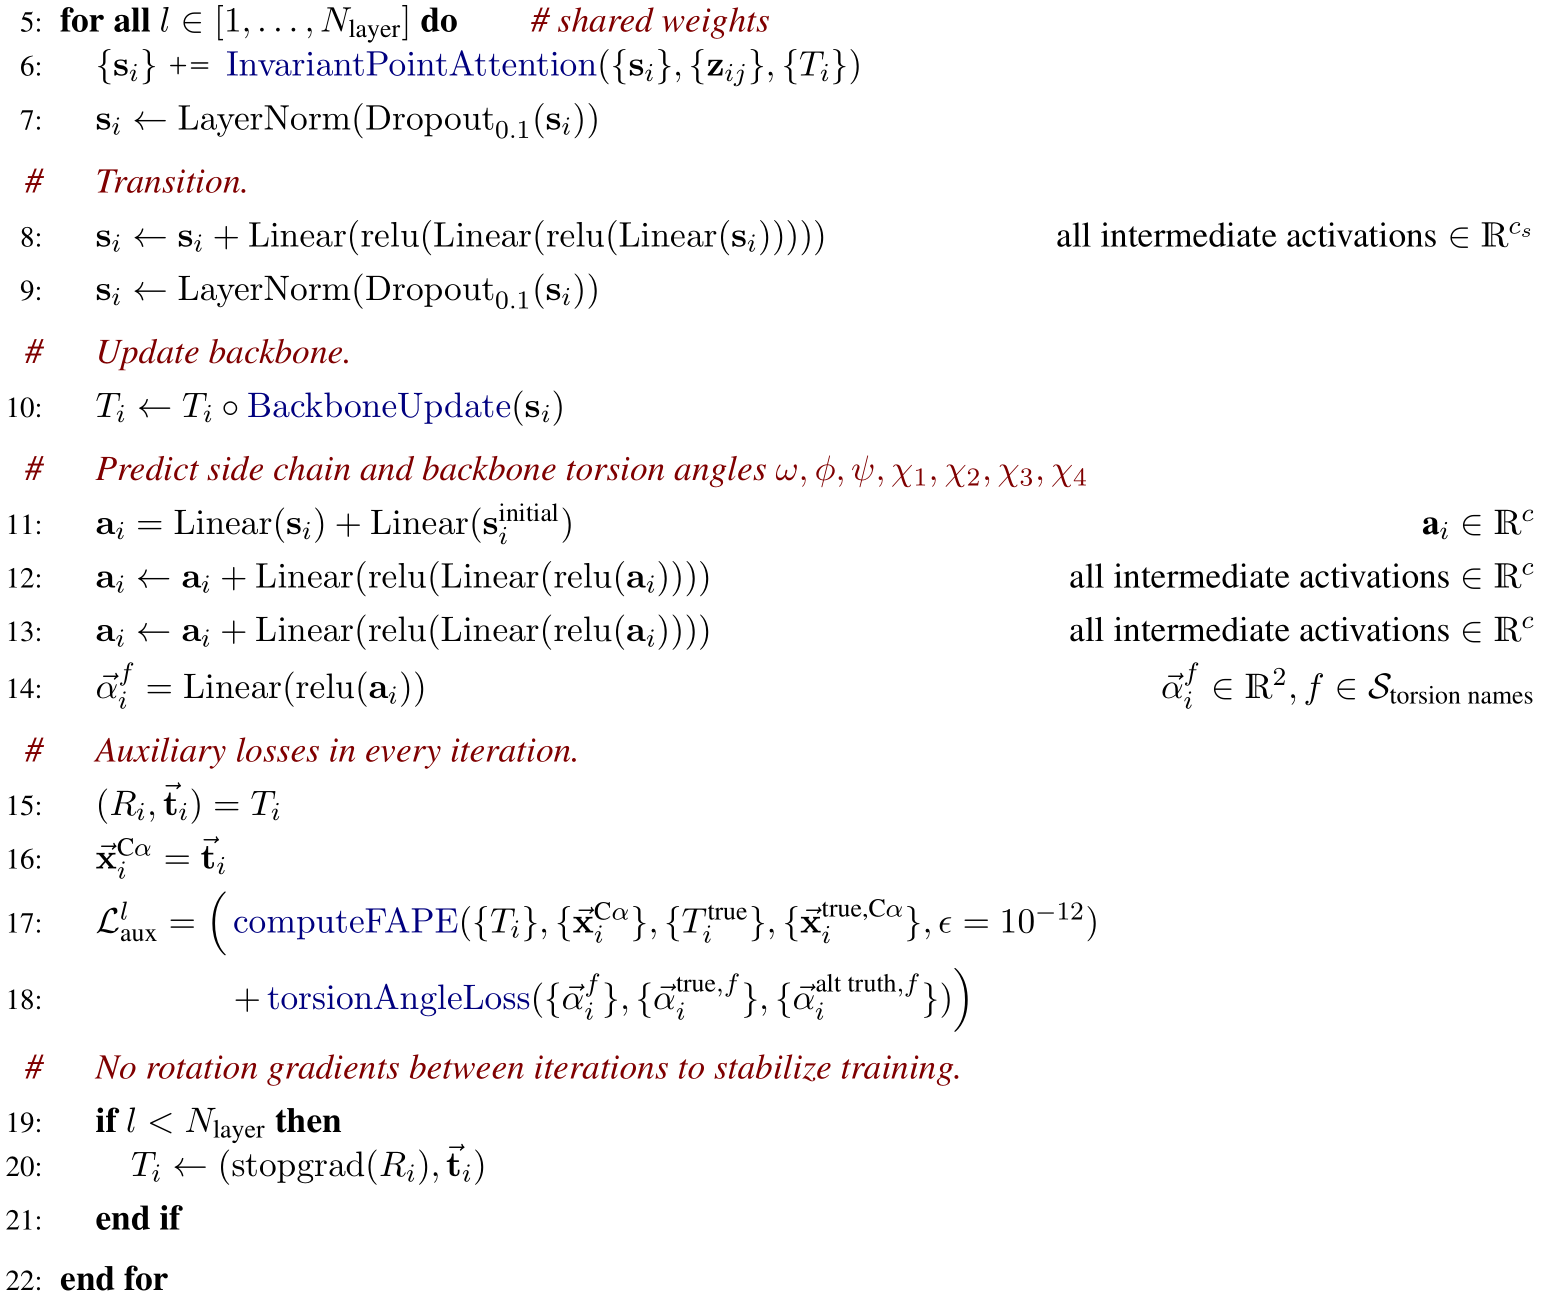
\includegraphics[height=0.9\textheight]{./imgs/algo20-part2.png}
\end{center}
\end{frame}

\begin{frame}[label={sec:org244dd17}]{Structure Module: Algorithm Part 3 \cite{jumperHighlyAccurateProtein2021}}
\begin{center}
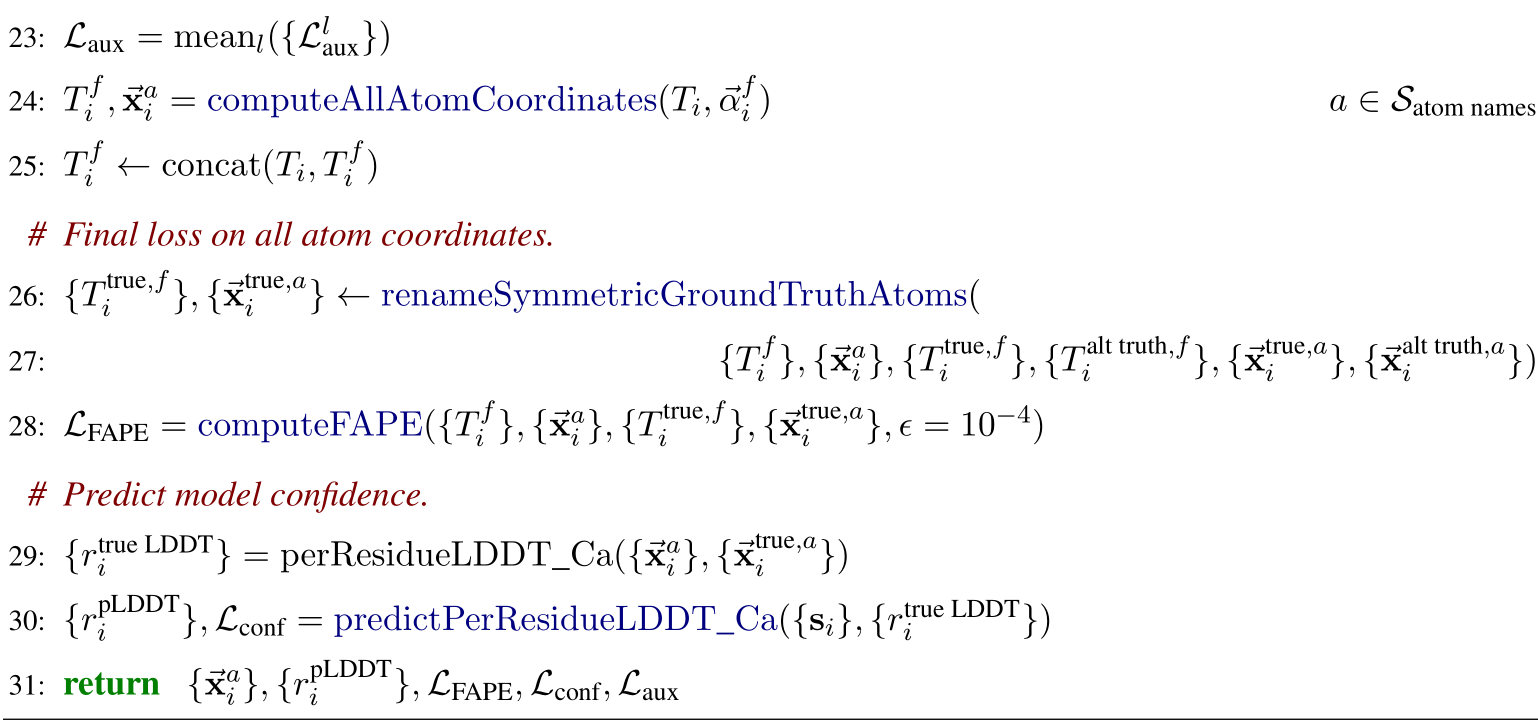
\includegraphics[width=.9\linewidth]{./imgs/algo20-part3.png}
\end{center}
\end{frame}

\begin{frame}[label={sec:org4ebcfad}]{Table 2 Rigid atomic groups from torsion angles \cite{jumperHighlyAccurateProtein2021}}
\begin{center}
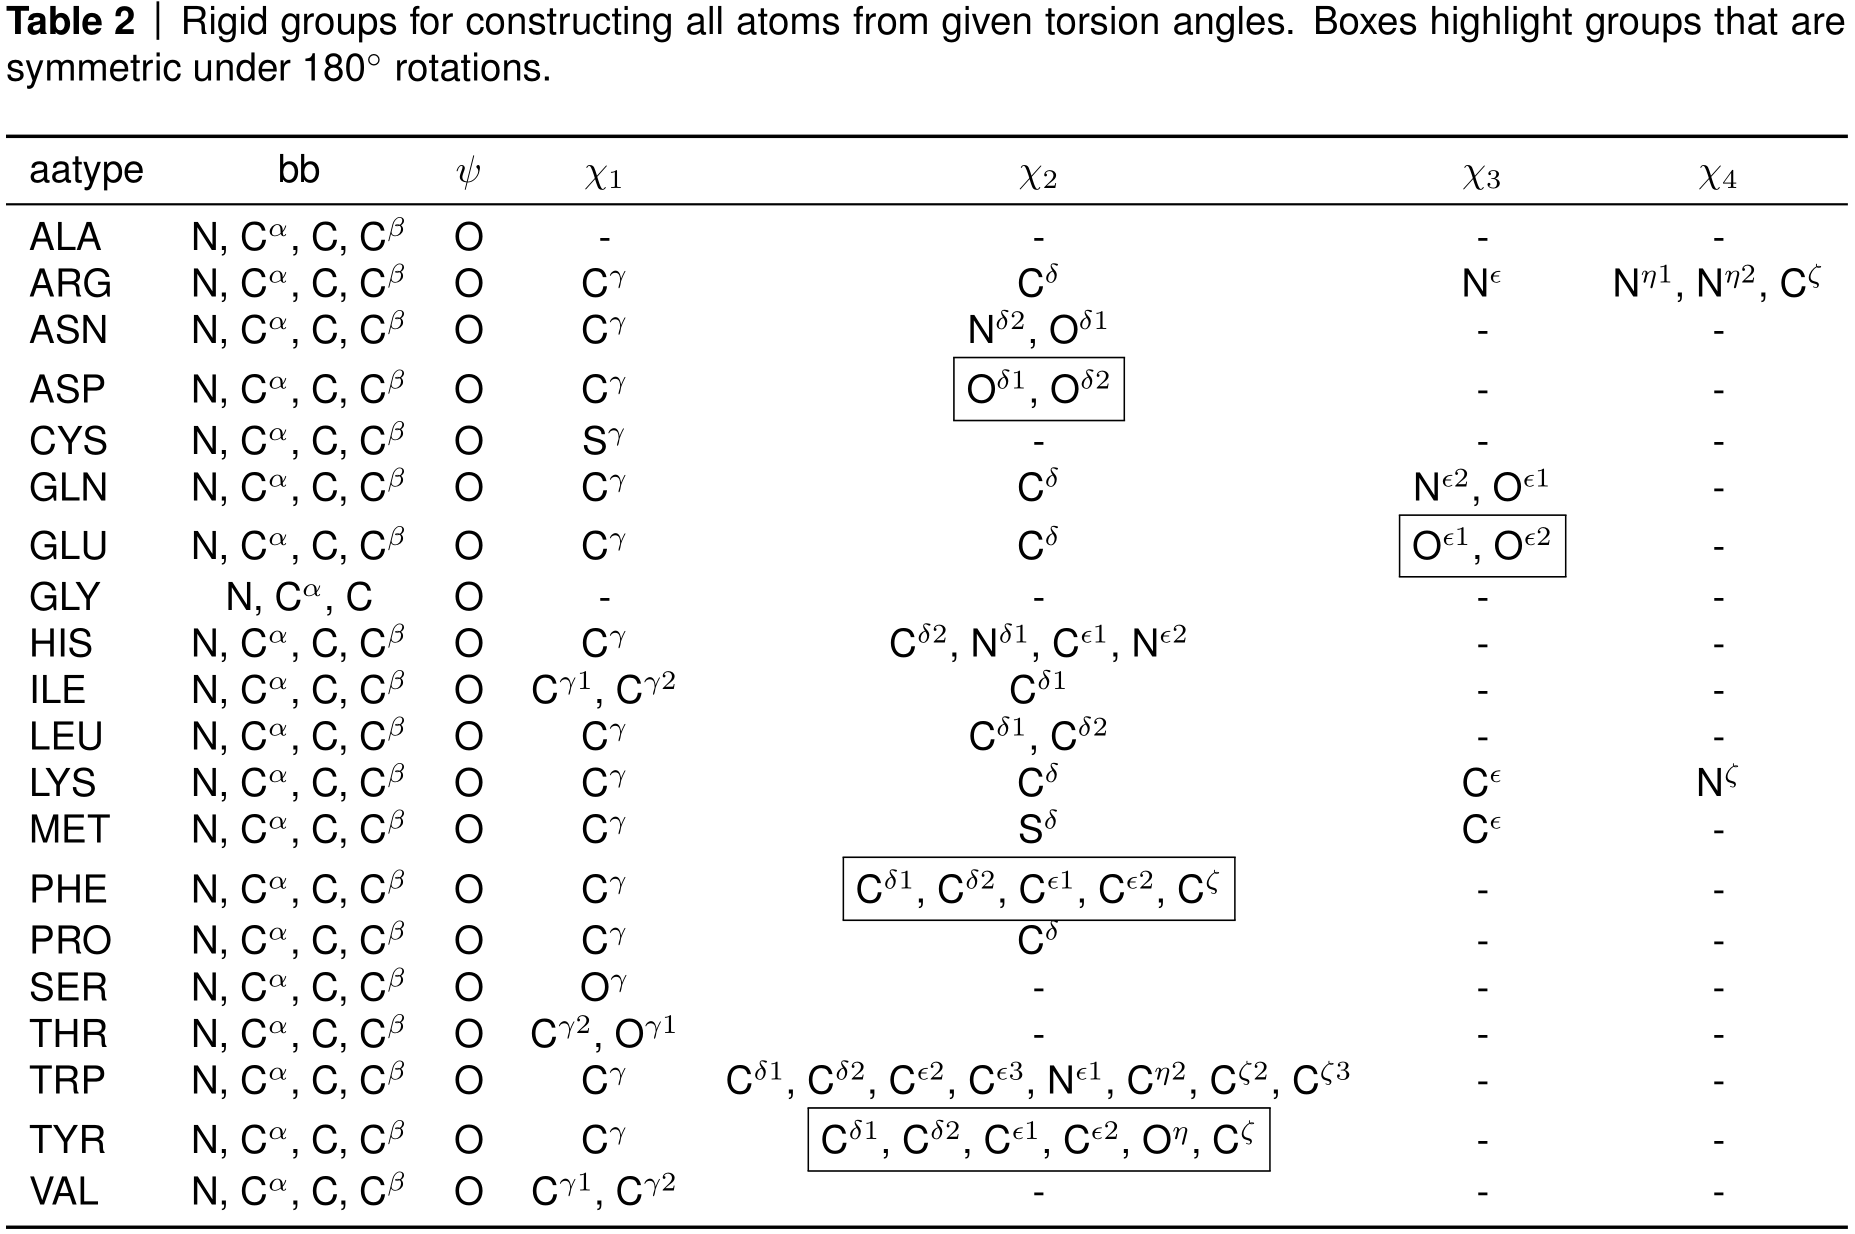
\includegraphics[height=0.9\textheight]{./imgs/table2_rigid_atom_groups.png}
\end{center}
\end{frame}

\begin{frame}[label={sec:org838c7f4}]{Algorithm 21 Frame construction from ground truth atom positions \cite{jumperHighlyAccurateProtein2021}}
\begin{center}
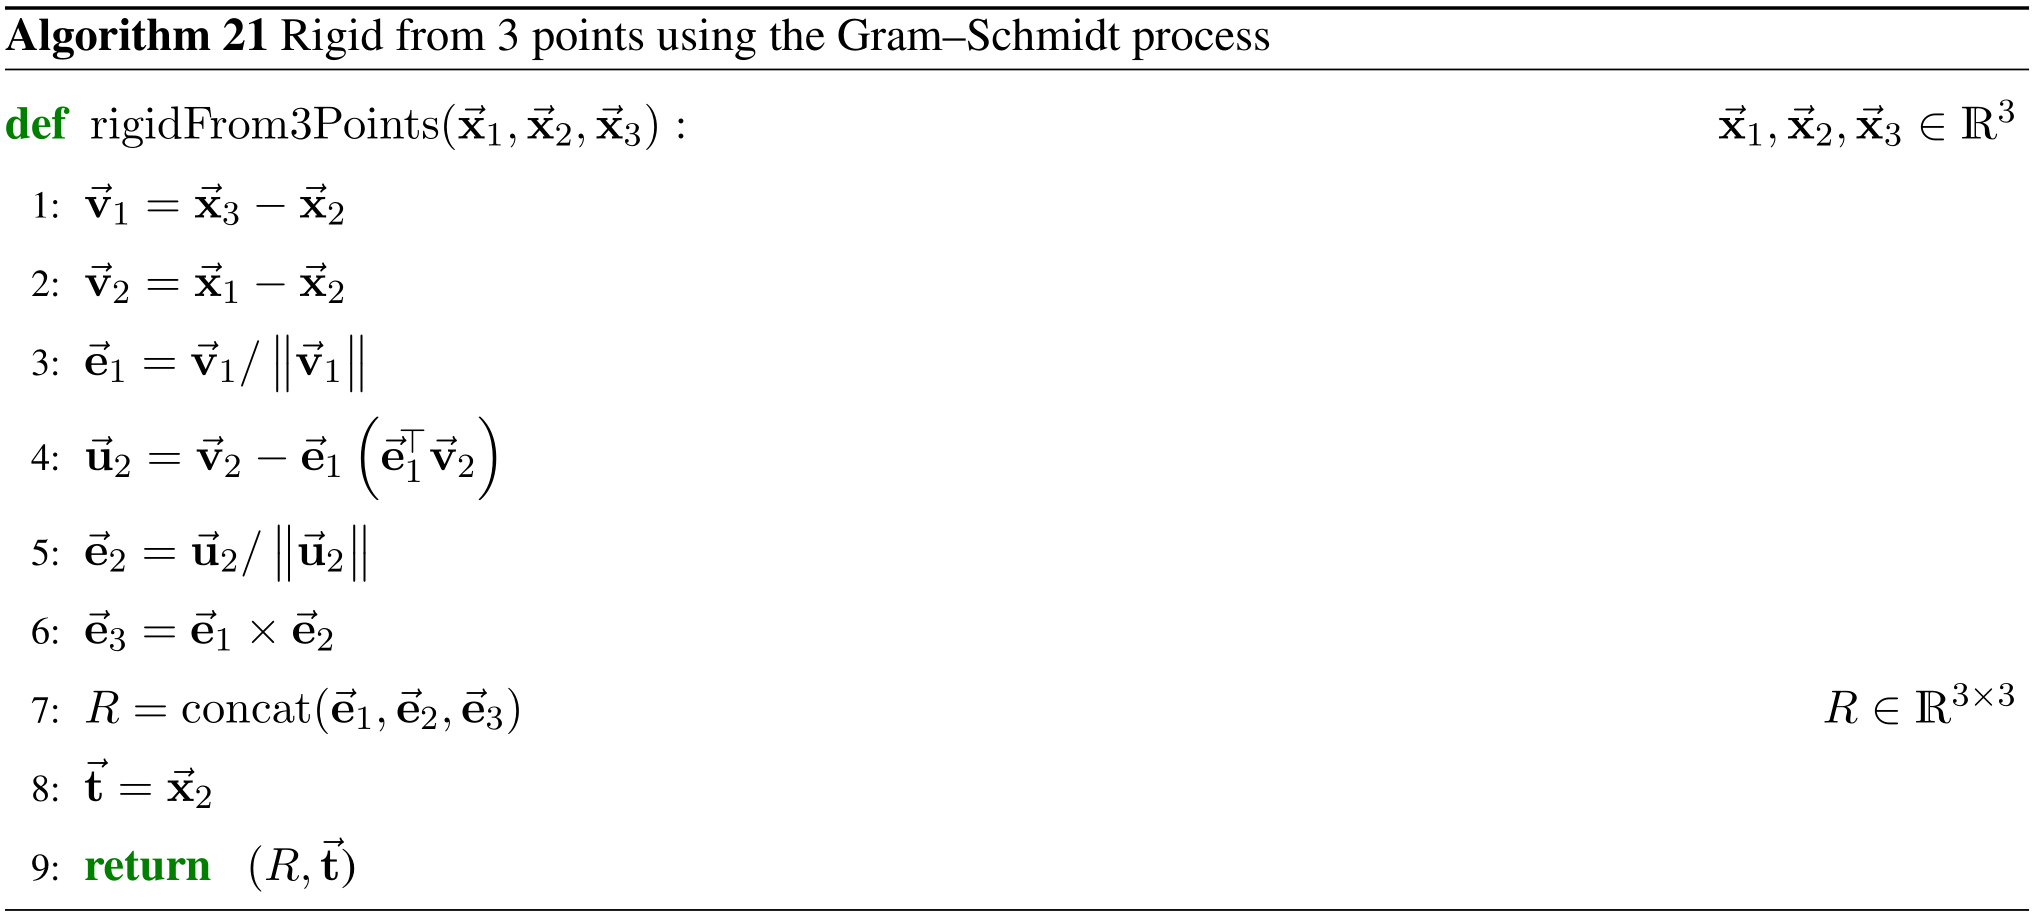
\includegraphics[width=0.9\textwidth]{./imgs/algo21_gram_schmidt.png}
\end{center}
\end{frame}
\begin{frame}[label={sec:org0923eb0}]{Algorithm 22 Invariant point attention (IPA) \cite{jumperHighlyAccurateProtein2021}}
\begin{center}
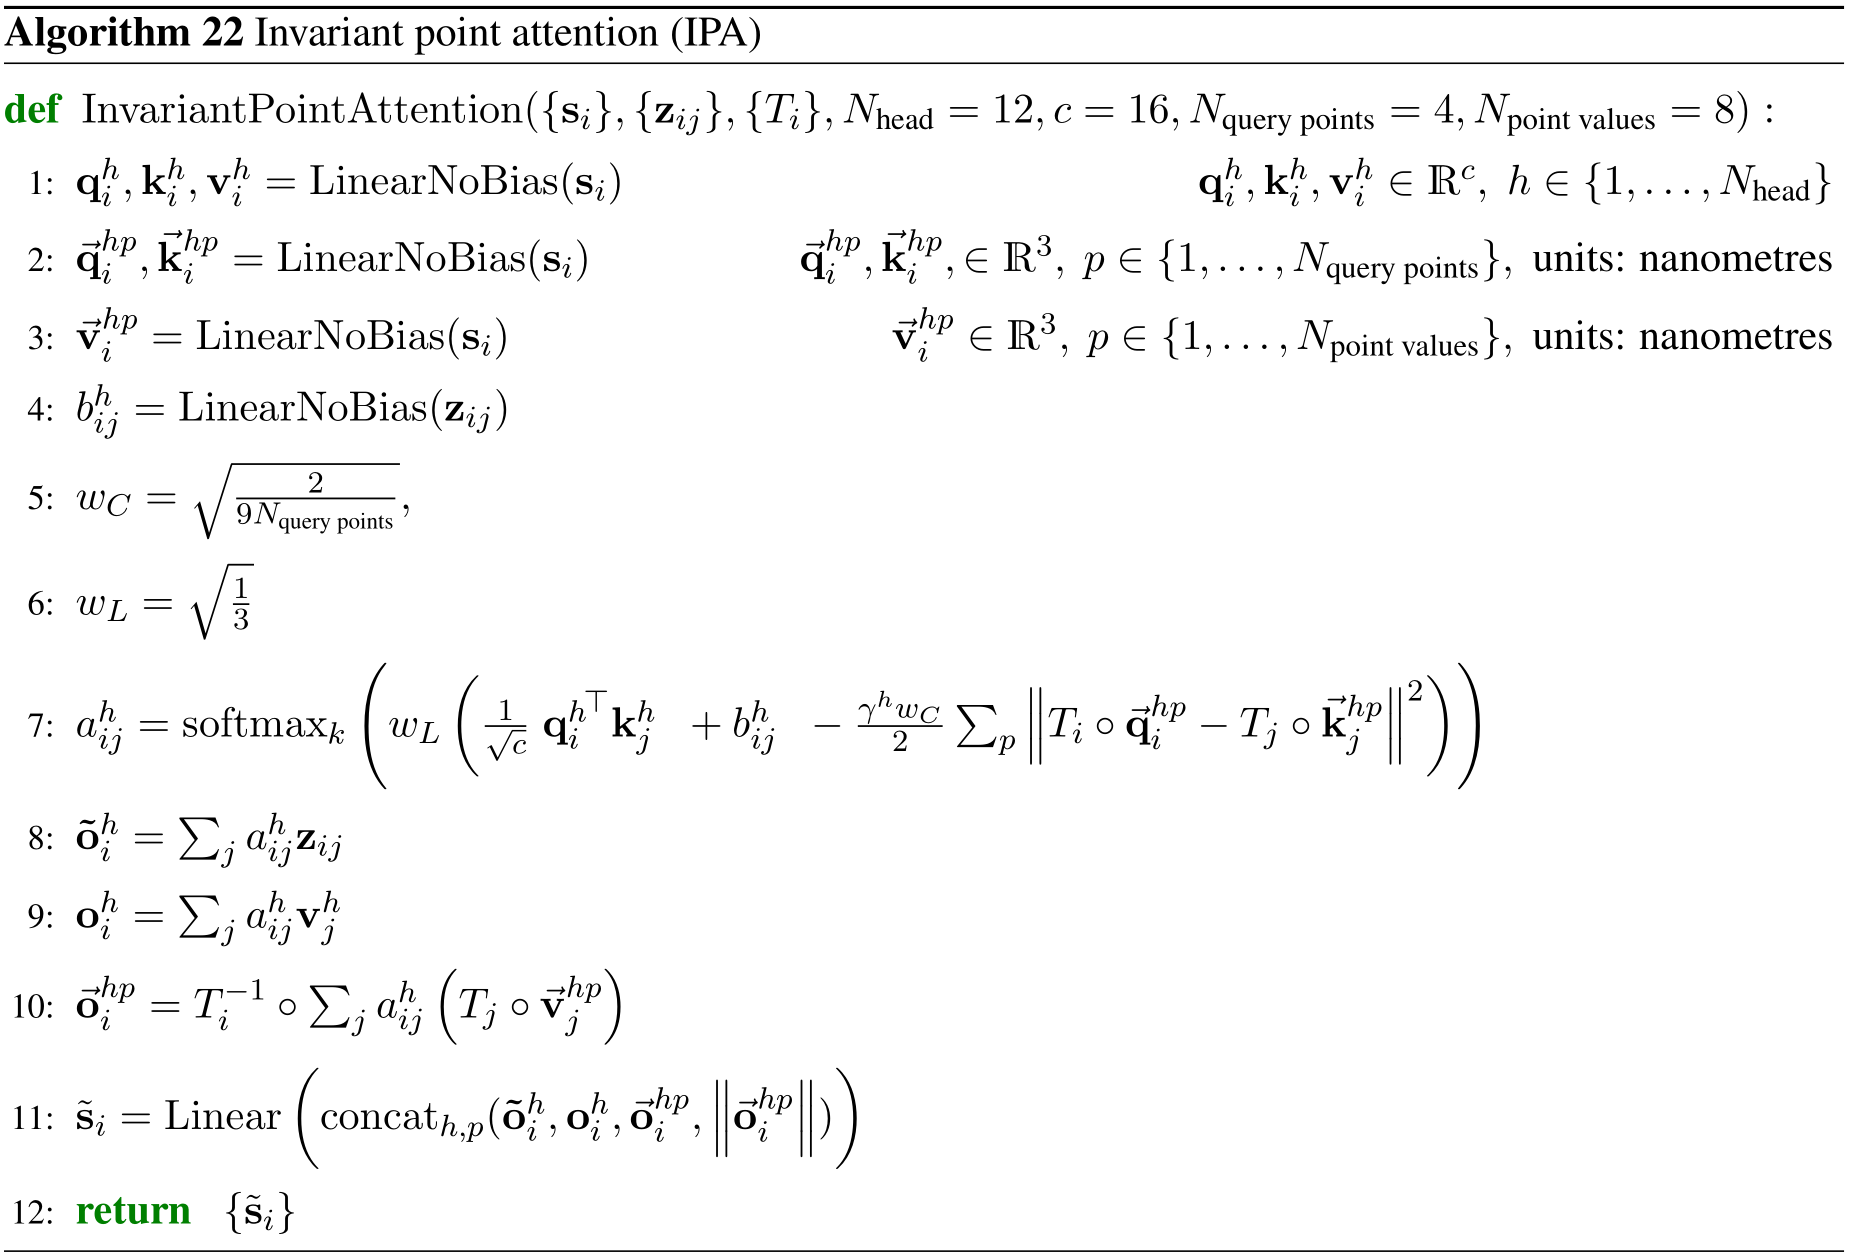
\includegraphics[height=0.9\textheight]{./imgs/algo22_ipa.png}
\end{center}
\end{frame}

\begin{frame}[label={sec:org4b73fff}]{Algorithm 23 Backbone update \cite{jumperHighlyAccurateProtein2021}}
\begin{center}
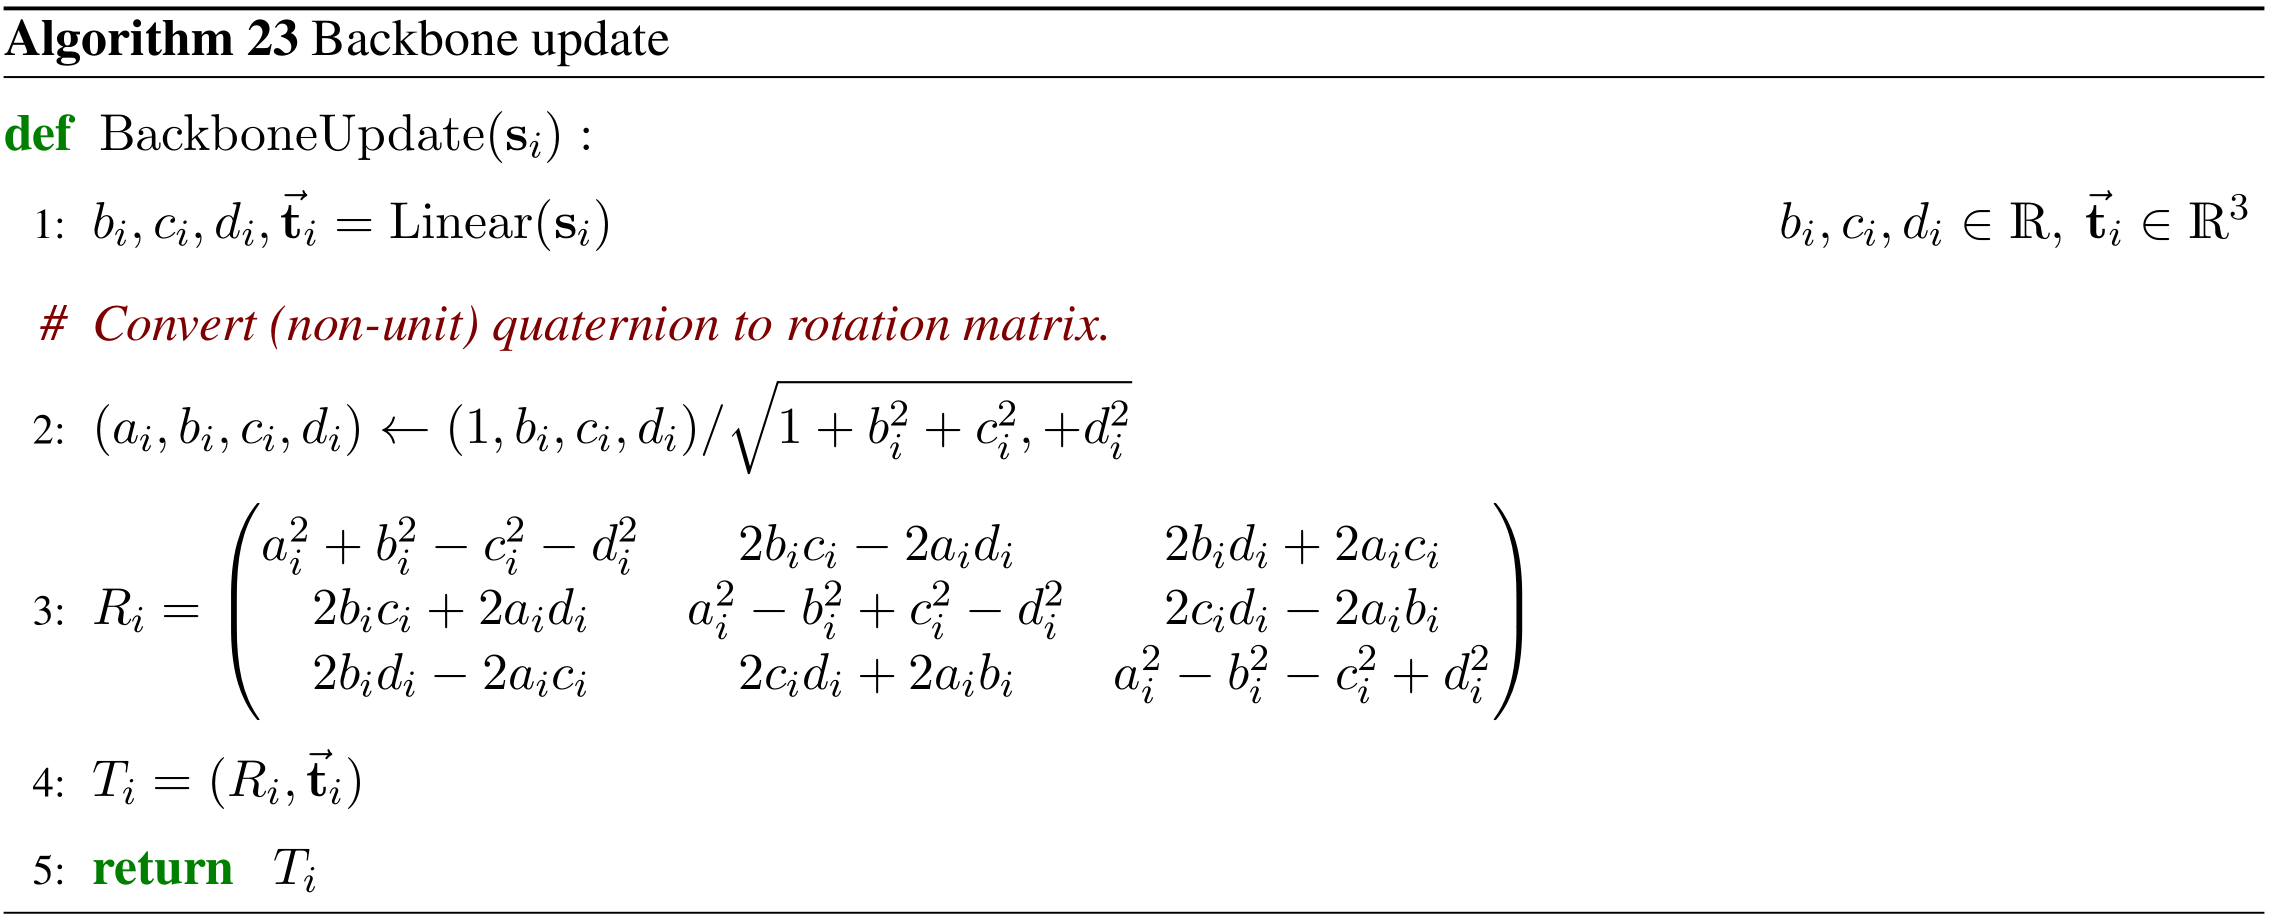
\includegraphics[width=.9\linewidth]{./imgs/algo23_backbone-update.png}
\end{center}
\end{frame}
\begin{frame}[label={sec:org42ddf21}]{Algorithm 24 Compute all atom coordinates \cite{jumperHighlyAccurateProtein2021}}
\begin{center}
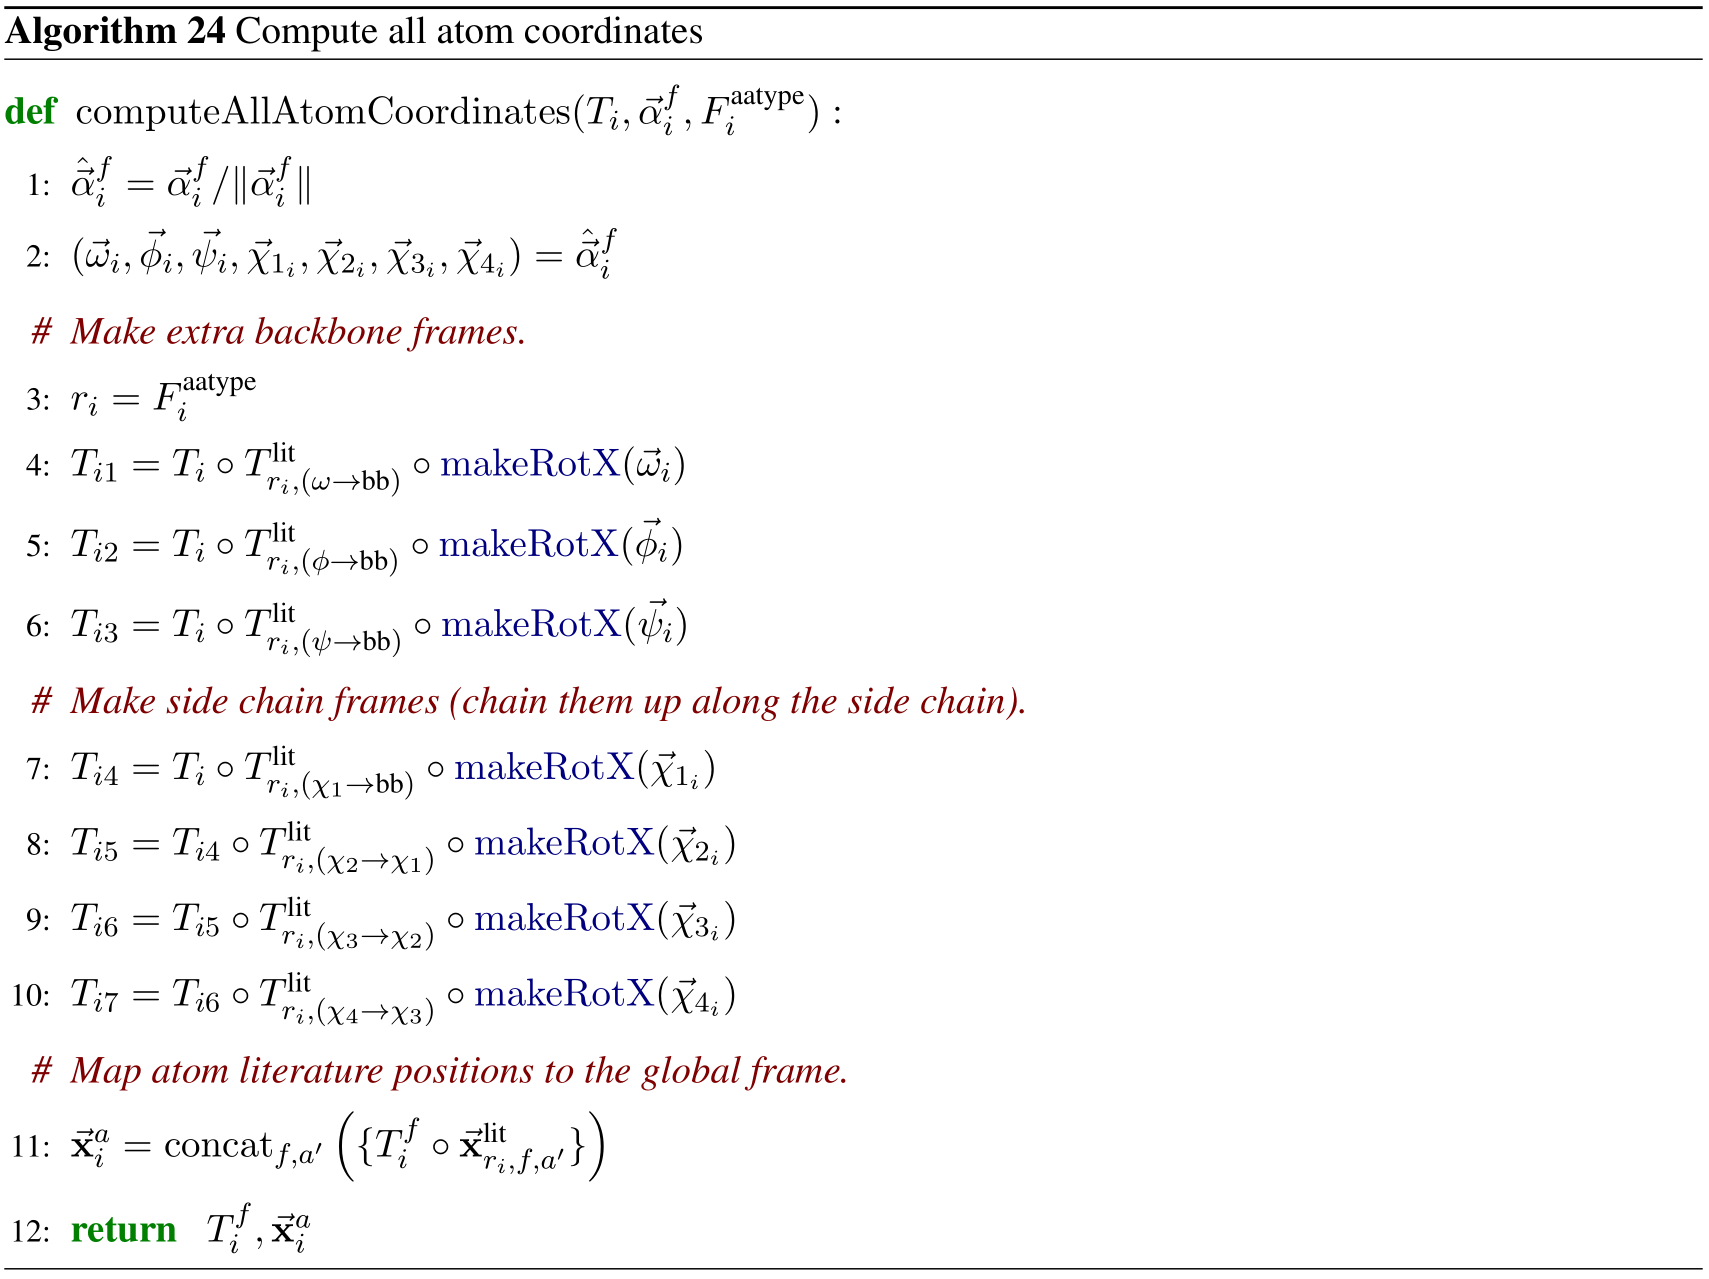
\includegraphics[height=0.9\textheight]{./imgs/algo24_all-atom-coords-algo.png}
\end{center}
\end{frame}
\begin{frame}[label={sec:org893ab32}]{Algorithm 25 Make a transformation that rotates around the x-axis \cite{jumperHighlyAccurateProtein2021}}
\begin{center}
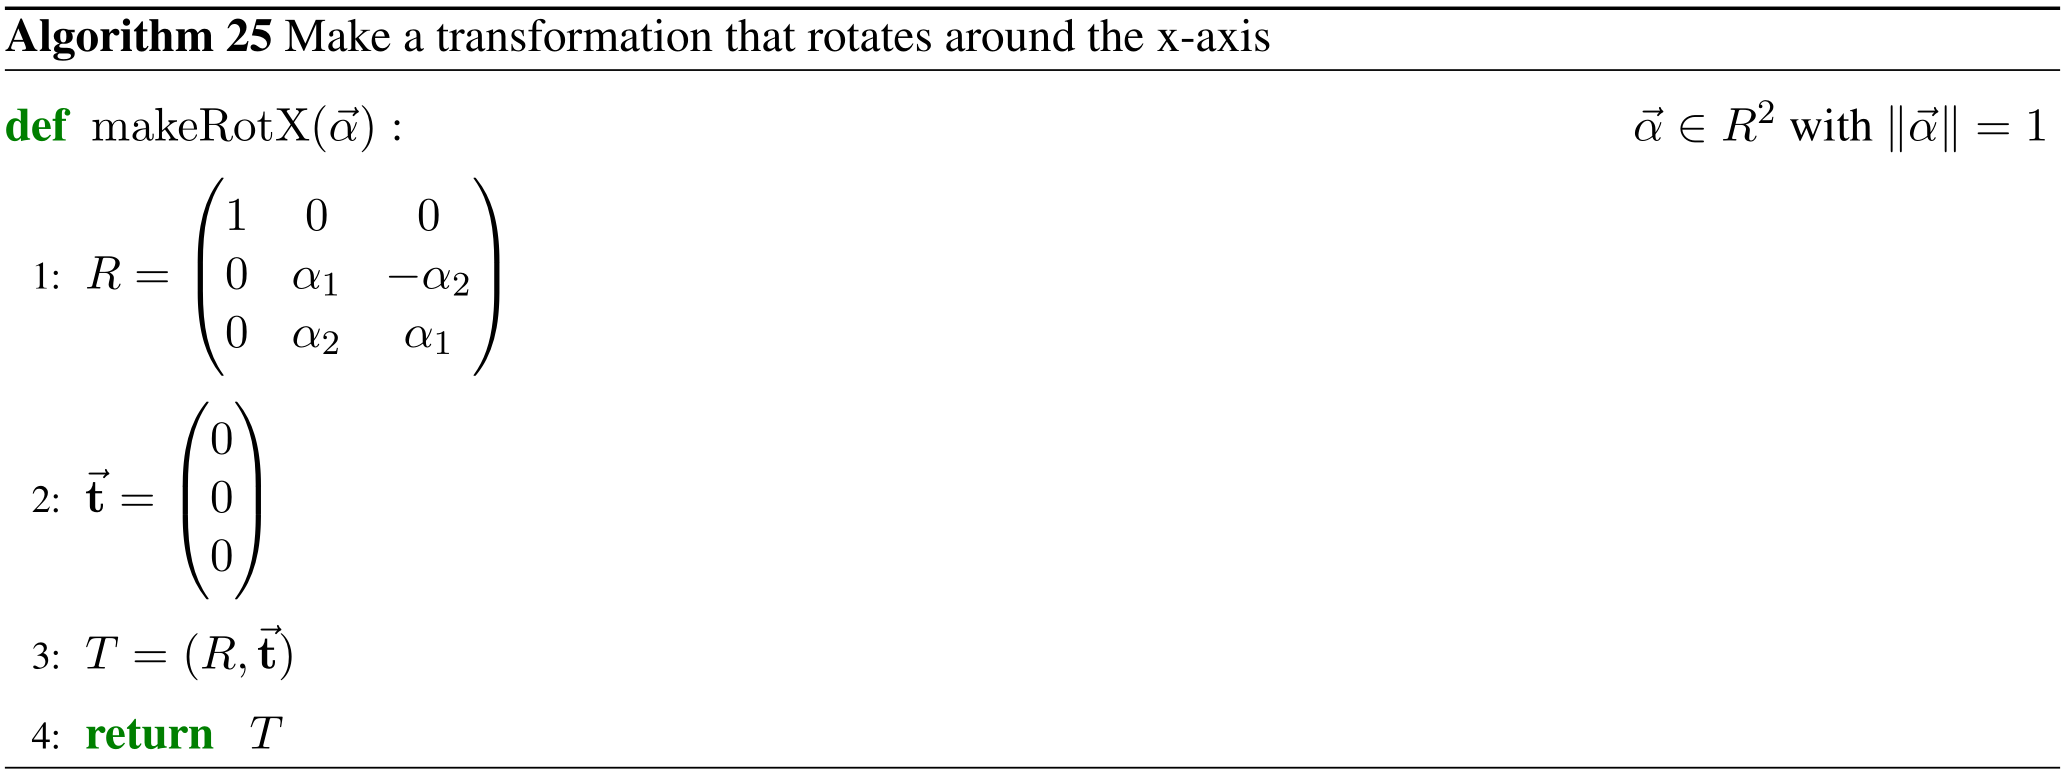
\includegraphics[width=.9\linewidth]{./imgs/algo25_xaxis-transform.png}
\end{center}
\end{frame}
\begin{frame}[label={sec:orge876001}]{Table 3 Ambiguous atom renaming swaps \cite{jumperHighlyAccurateProtein2021}}
\begin{center}
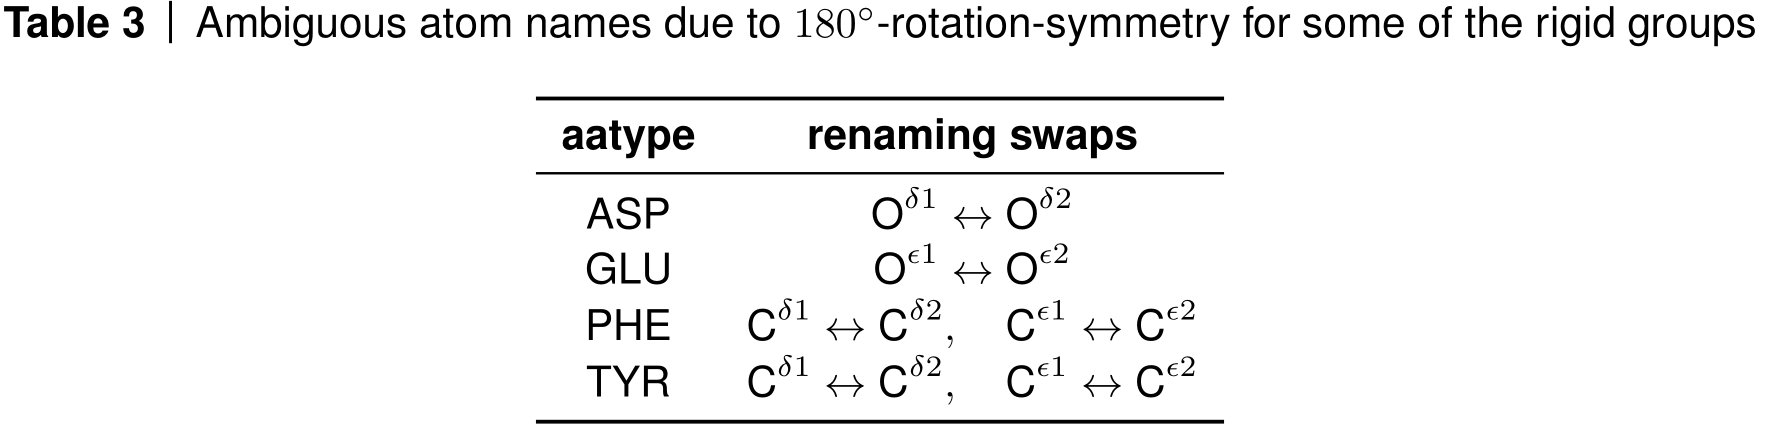
\includegraphics[width=\textwidth]{./imgs/table3_atom_renaming.png}
\end{center}
\end{frame}

\begin{frame}[label={sec:org96c8ffd}]{Algorithm 26 Rename symmetric ground truth atoms \cite{jumperHighlyAccurateProtein2021}}
\begin{center}
\includegraphics[width=.9\linewidth]{./imgs/algo26_rename-truth-atoms.png}
\end{center}
\end{frame}
\begin{frame}[label={sec:orgd19777b}]{Distograms \cite{jumperHighlyAccurateProtein2021}}
\begin{figure}[htbp]
\centering
\includegraphics[width=0.9\textwidth]{./imgs/distogram_example.png}
\caption{Example Distogram \protect\cite{seniorImprovedProteinStructure2020}}
\end{figure}
\end{frame}
\begin{frame}[label={sec:org598b501}]{Amber Relaxation}
\end{frame}
\subsection*{Loss Functions}
\label{sec:org0e74be0}
\begin{frame}[label={sec:org447ccae}]{Loss Functions  \cite{jumperHighlyAccurateProtein2021}}
\begin{center}
\includegraphics[width=.9\linewidth]{./imgs/loss-eq.png}
\end{center}

\begin{itemize}
\item weighted sum
\item weighted to reduce importance of short sequences
\end{itemize}
\end{frame}

\begin{frame}[label={sec:org8450db3}]{Loss Functions \& Auxillary Heads \cite{jumperHighlyAccurateProtein2021}}
\begin{enumerate}
\item Side chain and backbone torsion angle loss (sec. 1.9.1)
\item Frame aligned point error (FAPE) (sec. 1.9.2)
\begin{itemize}
\item Configurations with FAPE(X,Y) = 0 (sec. 1.9.4)
\item Metric properties of FAPE (sec. 1.9.5)
\end{itemize}
\item Chiral properties of AlphaFold and its loss (sec. 1.9.3)
\begin{itemize}
\item transforms \(T_i\) are variant under reflection (see eq. 11 to 17)
\item atom positions via backbone frames and \(\chi\) angles
\end{itemize}
\item Model confidence prediction (pLDDT) (sec. 1.9.6)
\item TM-score prediction (sec. 1.9.7)
\item Distogram prediction (sec. 1.9.8)
\item Masked MSA prediction (sec. 1.9.9)
\item "Experimentally resolved" prediction (sec. 1.9.10)
\item Structural violations (sec. 1.9.11)
\end{enumerate}
\end{frame}

\begin{frame}[label={sec:orga018bae}]{Algorithm 27 Side chain and backbone torsion angle loss \cite{jumperHighlyAccurateProtein2021}}
\begin{center}
\includegraphics[width=.9\linewidth]{./imgs/algo27_sidechain-backbonetorsion-loss.png}
\end{center}
\end{frame}
\begin{frame}[label={sec:orgc33c6d3}]{Loss Functions: FAPE}
\begin{figure}[htbp]
\centering
\includegraphics[width=.9\linewidth]{./imgs/algo28_fape.png}
{Algorithm 28 cite:jumperHighlyAccurateProtein2021}
\end{figure}


\begin{itemize}
\item Variation of commonly used root-mean-squared deviation (RMSD) of atomic positions
\item not invariant to reflections, preventing proteins of the wrong chirality. \cite{rubieraAlphaFoldHereWhat}, \cite{jumperHighlyAccurateProtein2021}
\end{itemize}
\end{frame}

\begin{frame}[label={sec:org304bf94}]{Algorithm 29 Predict model confidence pLDDT \cite{jumperHighlyAccurateProtein2021}}
\begin{center}
\includegraphics[width=.9\linewidth]{./imgs/algo29_confidence-pLDDT.png}
\end{center}
\end{frame}
\begin{frame}[label={sec:orge9fb894}]{TM-score prediction  \cite{jumperHighlyAccurateProtein2021}}
\begin{itemize}
\item Global superposition metric of \(C_\alpha\) atoms (eqs. 31 - 33)
\begin{enumerate}
\item approximated (eqs. 34-36)
\item Probabilistic lower-bound maximum-of-expectation score (eqs. 37-38)
\item approximated TM-score using pairwise \(C_\alpha\) based computation (\(e_{ij}\) matrix) and above (see eq. 39 and adjacent text)
\item TM-score of any residue subset \(D\) can be computed (eq. 40)
\begin{itemize}
\item can also be used to estimate GDT, FAPE, RMSD (using \(e_{ij}\)) matrix (not done)
\item used for confident domain packing visualizations
\end{itemize}
\end{enumerate}
\end{itemize}
\end{frame}

\begin{frame}[label={sec:org009ecd7}]{Distogram prediction  \cite{jumperHighlyAccurateProtein2021}}
\begin{itemize}
\item (eq. 41)
\end{itemize}
\end{frame}
\begin{frame}[label={sec:org80aeec3}]{Masked MSA prediction  \cite{jumperHighlyAccurateProtein2021}}
\end{frame}
\begin{frame}[label={sec:org1425f9b}]{"Experimentally resolved" prediction (fine tuning) \cite{jumperHighlyAccurateProtein2021}}
\end{frame}
\begin{frame}[label={sec:orgfce5f2e}]{Structural violations (fine tuning)  \cite{jumperHighlyAccurateProtein2021}}
\end{frame}
\section*{Training \& Inference Details}
\label{sec:orgcb95690}
\subsection*{Recycling iterations}
\label{sec:org7c0fa47}
\begin{frame}[label={sec:org1f655fb}]{Algorithm 30 Generic recycling inference procedure \cite{jumperHighlyAccurateProtein2021}}
\begin{center}
\includegraphics[width=.9\linewidth]{./imgs/algo30_recycling.png}
\end{center}
\end{frame}
\begin{frame}[label={sec:org3a0fdc1}]{Algorithm 31 Generic recycling training procedure \cite{jumperHighlyAccurateProtein2021}}
\begin{center}
\includegraphics[width=.9\linewidth]{./imgs/algo31_generic-recycling.png}
\end{center}
\end{frame}
\begin{frame}[label={sec:orgef69377}]{Algorithm 32 Embedding of evoformer and structure module outputs for recycling \cite{jumperHighlyAccurateProtein2021}}
\begin{center}
\includegraphics[width=.9\linewidth]{./imgs/algo32_recycling-embedding.png}
\end{center}
\end{frame}
\begin{frame}[label={sec:org4f28bc1}]{Training stages  \cite{jumperHighlyAccurateProtein2021}}
\end{frame}
\begin{frame}[label={sec:org3d85acc}]{MSA resampling and ensembling  \cite{jumperHighlyAccurateProtein2021}}
\end{frame}
\begin{frame}[label={sec:org7e91a0c}]{Optimization details  \cite{jumperHighlyAccurateProtein2021}}
\begin{itemize}
\item Adam \(\italic{lr} == 10^{-3}, \beta_1 = 0.9, \beta_2 = 0.999, \epsilon = 10^{-6}\)
\begin{itemize}
\item lr warm-up for \(0.128 \dot 10^6\) samples, increase again by \(0.65 after 6.4 \dot 10^6\) samples
\end{itemize}
\item batch: 128
\item gradient clipping by global norm (per parameter*sample) of 0.1
\end{itemize}
\end{frame}

\begin{frame}[label={sec:org186622e}]{Parameters initialization  \cite{jumperHighlyAccurateProtein2021}}
\end{frame}
\begin{frame}[label={sec:org423292d}]{Loss clamping details  \cite{jumperHighlyAccurateProtein2021}}
\end{frame}
\begin{frame}[label={sec:orgba1dbc6}]{Dropout details  \cite{jumperHighlyAccurateProtein2021}}
\end{frame}
\begin{frame}[label={sec:org09eaaef}]{Evaluator setup  \cite{jumperHighlyAccurateProtein2021}}
\end{frame}
\begin{frame}[label={sec:orgbac25a3}]{Reducing the memory consumption  \cite{jumperHighlyAccurateProtein2021}}
\end{frame}
\section*{Results}
\label{sec:org7c7a457}
\begin{frame}[label={sec:org2d131a6}]{CASP14 Assessment \cite{jumperHighlyAccurateProtein2021}}
They did well
\end{frame}
\begin{frame}[label={sec:org5d63886}]{Ablation Studies \cite{jumperHighlyAccurateProtein2021}}
Baseline for all ablation models: Full model without noisy-student self-attention  
Ablations:
\begin{enumerate}
\item With noisy-student self-distillation training
\item No templates
\item No raw MSA (use MSA pairwise frequencies)
\item No triangles, biasing, or gating (use axial attention)
\item No recycling
\item No IPA (use direct projection)
\item No invariant IPA \& no recycling
\item No end-to-end structure gradients (keep auxiliary heads)
\item No auxiliary distogram head
\item No auxiliary masked MSA head
\end{enumerate}
\end{frame}

\begin{frame}[label={sec:org7b72ead}]{Ablation Results (in main paper) \cite{jumperHighlyAccurateProtein2021}}
\begin{center}
\includegraphics[height=0.9\textheight]{./imgs/ablation_results.png}
\end{center}
\end{frame}
\begin{frame}[label={sec:orgec8d846}]{Ablation Results \cite{jumperHighlyAccurateProtein2021}}
\begin{center}
\includegraphics[height=0.9\textheight]{./imgs/fig10_ablation_results.png}
\end{center}
\end{frame}

\begin{frame}[label={sec:org86e5026}]{Network Probing \cite{jumperHighlyAccurateProtein2021}}
todo
\end{frame}

\begin{frame}[label={sec:org4f1d4fc}]{Novel Folds}
They did well
\end{frame}

\begin{frame}[label={sec:orgaa3cb85}]{Attention Visualization \cite{jumperHighlyAccurateProtein2021}}
todo
\end{frame}

\begin{frame}[label={sec:org90e4014}]{Additional Results \cite{jumperHighlyAccurateProtein2021}}
todo
\end{frame}

\section*{Biblio}
\label{sec:org3e23c2b}
\begin{frame}[fragile,allowframebreaks,label=]{Bibliography}
\printbibliography
\end{frame}
\end{document}